\documentclass[a4paper, 12pt]{report}
\usepackage[latin1]{inputenc}
\usepackage[english]{babel}
%\usepackage[T1]{fontenc}
\usepackage{graphicx}
\usepackage{float}
\usepackage[centertags]{amsmath}
\usepackage{amsfonts}
\usepackage{amssymb}
\usepackage{amsthm}
\usepackage{newlfont}
\usepackage{fancyhdr}
\usepackage{tesisty}
\usepackage[table,xcdraw]{xcolor}
\usepackage{subfig}
\usepackage{textcomp}
\usepackage{gensymb}
\usepackage{url}
\usepackage{lscape}

%-------------------------------
% DEFINIZIONE DEGLI ENVIRONMENT
%-------------------------------

\newtheorem{obs}{Osservazione}[section]
\newenvironment{oss}
    {\begin{obs}\begin{normalfont}}
    {\hfill $\square \!\!\!\!\checkmark$ \end{normalfont}\end{obs}}

\newtheorem{pro}{Problema}[chapter]
\newenvironment{prob}
    {\begin{pro}\begin{normalfont}}
    {\hfill $\spadesuit$ \end{normalfont}\end{pro}}

\newtheorem{teor}{Teorema}[section]
\newenvironment{teorema}
    {\begin{teor}\textit }
    {\hfill  \end{teor}}

\newtheorem{defn}{Definizione}[section]
\newenvironment{de}
    {\begin{defn}\begin{normalfont}}
    {\hfill $\clubsuit$ \end{normalfont}\end{defn}}

%-----------------------------
% CONFIGURAZIONE DELLA PAGINA
%-----------------------------

\hfuzz2pt % Don't bother to report over-full boxes if over-edge is < 2pt

\fancypagestyle{plain}{
\fancyhead{}\renewcommand{\headrulewidth}{0pt} } \pagestyle{fancy}
\renewcommand{\chaptermark}[1]{\markboth{\small CAP. \thechapter \textit{ #1}} {} }
\renewcommand{\sectionmark}[1]{\markright{\small  \thesection \textit{ #1}} {} }
\voffset=-20pt    % distanza tra il limite superiore del foglio e l'intestazione
\headsep=40pt     % distanza  l'intestazione ed il testo del corpo
\hoffset=0 pt     % misura equivalente al margine sinistro
\textheight=620pt % altezza del corpo del testo
\textwidth=435pt  % larghezza del corpo del testo
\footskip=40pt    % distanza tra il testo del corpo ed il pie' di pagina
\fancyhead{}      % cancella qualsiasi impostazione per l'intestazione
\fancyfoot{}      % cancella qualsiasi impostazione per il pie' di pagina
\headwidth=435pt  % larghezza del'intestazione e del pie' di pagina
\fancyhead[R]{\rightmark} \fancyfoot[L]{\leftmark}
\fancyfoot[R]{\thepage}
\renewcommand{\headrulewidth}{0.3pt}   % spessore della linea dell'intestazione
\renewcommand{\footrulewidth}{0.3pt}   % spessore della linea del pi�di pagina

\numberwithin{equation}{section}
\renewcommand{\theequation}{\thesection.\arabic{equation}}


 
\begin{document}


\dedicate{'Crescat scientia vita excolatur'}

\corso{ICT and Internet Engineering} 
\titoloTesi{Analysis of drone's micro-Doppler signature with FMCW radars}
\anno{A.A. 2020/2021}
\relatore{Prof. Mauro Leonardi}
\autore{Ivan Riolo}
\matricola{}
%\correlatore{Correlatore}
\baselineskip=25pt
\intestazione
%------------------------------------------------
% INTRODUZIONE E RINGRAZIAMENTI (NON MODIFICARE)
%------------------------------------------------

\fancypagestyle{plain}{
\fancyhead{}\renewcommand{\headrulewidth}{0pt} } \pagestyle{fancy}
\renewcommand{\chaptermark}[1]{\markboth{\small Cap. \thechapter \textit{ #1}} {} }
\renewcommand{\sectionmark}[1]{\markright{\small  \S \thesection \textit{ #1}} {} }
\voffset=-20pt                         % distanza tra il limite superiore del foglio e l'intestazione
\headsep=40pt                          % distanza  l'intestazione ed il testo del corpo
\hoffset=0pt                           % misura equivalente al margine sinistro
\textheight=620pt                      % altezza del corpo del testo
\textwidth=435pt                       % larghezza del corpo del testo
\footskip=40pt                         % distanza tra il testo del corpo ed il pie' di pagina
\fancyhead{}                           % cancella qualsiasi impostazione per l'intestazione
\fancyfoot{}                           % cancella qualsiasi impostazione per il pie' di pagina
\headwidth=435pt                       % larghezza del'intestazione e del pie' di pagina
\fancyhead[R]{\rightmark} \fancyfoot[L]{\leftmark}
\fancyfoot[R]{\thepage}
\renewcommand{\headrulewidth}{0.3pt}   % spessore della linea dell'intestazione
\renewcommand{\footrulewidth}{0.3pt}   % spessore della linea del pi�di pagina

\pagenumbering{Roman} \tableofcontents
\newpage

\pagenumbering{arabic}

\fancyhead[R]{Introduzione} \fancyfoot[L]{Introduzione}
\fancyfoot[R]{\thepage}

\include{Introduzione}

\fancyhf{} %elimina header/footer vecchi


\fancyhead[R]{\rightmark} \fancyhead[L]{\leftmark}
\fancyfoot[R]{\thepage}



%---------------------
% INCLUSIONE CAPITOLI
%---------------------


%capitolo1
\chapter{Introduction}
\section{General aspects}
The technological evolution in the field of micro aircraft brings multiple benefits in many field of applications. Many industrial sectors benefits from the use of these devices, some examples are agricultural engineering, package delivery, but also security and military industry. The main interest concerns especially drones that have four rotors, also called quadcopters. The rapid expansion of the drone industry for civil contexts has overwhelmed the regulations in the use of them in terms of safety and control. While in the military context the development of surveillance system keeps up with the evolution of drones, the same is not true for civilian surveillance and defense. Consequently, these tools can be used to carry out illegal actions and crimes without being easily thwarted with civil technologies but only with sophisticate and expensive systems. Is important to consider that in recent times the drone's technology has undergone an incredible development mainly in the civil field. In fact, the recent diffusion of drones for commercial use has undergone an exponential growth. \\ Mosts significant causes for the drones's success is the ease of use and the low cost. In fact, anyone nowadays can easily get and use a drone even without having any experience in this field. On the other hand, due to the incredible spread of drone, the first regulations are being born in this period such as the driving license, or the drone no fly zones \cite{survey}. These regulations are really difficult to verify and control in a simple way. The security aspect acquires greater importance as these devices are easily accessible and easy to use by anyone. In this way the drones are able to carry out many illegal actions in a simple way and allow ill-intentioned users to escape the controls of the police. So the drones are also a good instruments to carry out terrorism and illegal operations like transporting illegal objects, weapons, bombs, etc.\\ How it is possible to to contrast illegal action and put into practice the drones's regulations easily?\\
Considering the current development of commercial drones such as their velocity, their range and their battery duration, is very difficult to protect an area against unauthorized flying drone by using non military equipments. This denotes that there isn't an equal technological level for the side of civilian defence devices, so the imbalance between commercial drone and civilian defense technology is very great. So the infringements of the rules became difficult to detect and contrast. While in the military context drones have been used for several years and the technologies of contrast and protection are very advanced. Then obviously it is not possible to use military solutions in the civilian context, for a matter of high costs but above all for the security of the close people. While there is a large increase in documented and verified accidents due to civilian drones, as we can understand, on the other hand there is no simple civilian security system for drone defense. For example in the military technologies one of the less invasive techniques of drone neutralization is the jamming, that do not involve the use of physical weapons and the main objective is to interfere with the flight of the drone. Despite the absence of physical weapons in a civilian context, it cannot be used due to the interference caused to other communications. For example the existing wireless network system or wireless sensors network would be temporarily paralyzed. \\ The impossibility to use a jamming approach in presence of people is also due to the possible fall down of the drone, that in relation to it's velocity and it's mass can cause serious problems and incidents, also if we consider that it can transport explosive. \\ The detection solutions for drone defense are many and of different nature, each with its own pros and cons \cite{survey} \cite{uspace} \cite{robinradar1}. There is no single and complete solution, in fact, the use of several systems at the same time called hybrid systems is preferred. \\ The main attention of this thesis is put on the first phase of drone defense in civil context that is the detection phase and the technology investigated is the radar one. Several type of radars are used today to contrast drone also in civilian context but the cost of these devices is very high. The principal aim is to detect and to understand if there is a possible threat in the supervised area by means of a cost accessible radar technology. It's important to consider that the detection capability includes also the ability to identify an unauthorized drone. This means that detection instruments must be able to distinguish between drone and other flying object as birds, and then it must be capable to understand if the drone is legal or illegal, for example by analyzing it's flying path. Usually the contexts area in a civil environment is a crowded events such as concert or a sport event, where the large number of people makes security checks very difficult and exposes the context to a high terrorist attack risk. In these cases, the vulnerability to illegal drones used to carry explosives is very high. This is one of the most critical cases, but drone defense can be very useful even in less critical cases. For example, it could be very useful to block a drone carrying a symbol of violence capable of causing clashes and unrest, as happened several times during international sporting events characterized by political tensions. Another field of application of less critical case is the protection of privacy and confidentiality that doesn't cause serious risk to people safe but is at the same time important. For example an unauthorized drone can be used to spy a confidential site like industrial production site.\\ More close to individual context, can be the protection of individual houses or boat where people may have a significant need to protect their privacy. Another field of application could be the prisons, where drones could be used to transport objects from the outside. All these context are characterized by the need of low cost, portable and ease of use detection instruments that is not possible to find in the military solutions.\\ Some of the drone detection solutions used today are based on optical/thermal vision, radar, acoustic and radio frequencies technologies but these are characterized by high costs and complexity. The focus is put on the radar technologies and the aim is to find an optimal solution for all these cited civil context characterized by the presence of people near to the detection radar. The idea is to achieve low cost and low complexity solutions that permit to put radar technologies for drone defense in the market for civilian people considering that the possibility to use military system is eliminated.

\begin{figure}[h!]
    \centering
    \includegraphics[width=12cm]{imgs/Drone delivery.jpg}
    \caption{Quadcopter drone in package delivery.}
\end{figure}




\section{Motivations}
The motivations that drive the research and development of drone defense can be deduced from the documented cases of accidents and attacks on public safety that have been made by means of drones \cite{survey} \cite{uspace}. It is important to note that the drones we are talking about are not those used in war, but the simple commercial drones that can be purchased in any electronics store. There are many and different cases in which the defense against unauthorized drones is of significant importance. For simplicity we can divide the application cases into two large groups: military cases and civil cases. This is why it is important to evaluate the level of risk and the context in order to choose the appropriate defense technologies. Faced with a very high risk in a very large area such as in an airport, it is necessary to use a military-grade technology that therefore requires high costs and high complexity. Faced with a less extensive risk that concerns an area of limited size, as in the case of a public event, a civil defense technology becomes necessary and therefore it requires low cost but at the same time portability and ease to deploy/use. Several documented events highlight the need for a good defense against unauthorized use of drones are shown below \cite{survey}.
As for the military field, documented cases in airports show how traffic can be blocked by the presence of unauthorized drones near airport runway. For example in December 2018 at Gatwick Airport, the second largest airport in England, air traffic was blocked for a day due to the presence of unauthorized drone flying over the runaway. The instrument used for ATC (Air Traffic Control) in 2018 were unable to detect a very small object close to the instruments. The same thing happened at the Frankfurt Airport in Germany in May 2019 \cite{survey}. The drones managed to reach crucial areas for air traffic without being detected by the existing radar systems due to their small RCS and close proximity to the devices. Other dangerous events attributed to military-grade cases are attacks on public institutions. One of the most recent cases documented is the attack on Saudi Arabia's largest oil refinery in September 2019, using 10 explosives-carrying drones \cite{survey}. Obviously in this case of attack the drones were more sophisticated than simple commercial ones and were of military level. So it's preferable to use also a military grade level defense system in this cases because in a context like an airport or an oil refinery is possible to use expensive devices and complex solution to guarantee the security. \\ Let's now focus on the most significant cases for the purpose of the thesis, those concerning individual objectives or public events where it is not possible to use military-level equipment. A first documented case is the attack on the home of the Japanese prime minister in April 2015 \cite{survey}, where for obvious reasons it is not possible to install military protective equipment. Precisely in these conditions, the need for a portable, simple and low-cost detection system becomes very clear. Some examples of military-grade attacks carried out using commercial-grade drones are provided by the old Islamic State (IS). The first documented case that discloses the possibility of using common commercial drones to carry out attacks occurred in Syria in October 2016, when the IS murdered two Iranians using drones bought on Amazon \cite{survey}. This event makes the concept of how simple it is to carry out illegal actions by means of commercial drones very clear. There was also the first case of attempted assassination of a head of state by means of drone, that it's what happened to Venezuelan president Nicolas Maduro in August 2018 \cite{survey}. During a public event, two common commercial drones carrying bombs tried to hit it, fortunately it did not go well. For what concern the public events, one of the most famous case of non authorized drone was in October 2014 during the national football match Serbia-Albania: a drone invaded the playing field carrying a political-military symbol that caused serious clashes and unrest preventing the continuation of the game. \\ Given the enormous availability and the ever lower cost of commercial drones, the urgent need for detection devices of the same level is very clear. The same level means the ease of use, low cost and portability of detection systems. Considering that commercial drones can achieve velocities that goes from several km/h up to 140 km/h. %It's a problem also the too low velocity because it's necessary a radar with a very high resolution in frequency to detect them.
The maximum range achievable by a commercial controlled drone can vary from 2-3 km up to 10 km so the range is also an important parameter to design a radar instrument. Also the range in altitude, of about 6 km, is a critical parameter. Considering the small dimensions of a drone at this altitude is impossible to see it with naked eye. Especially in conditions of temporary events a quick installation becomes possible thanks to the ease of deployment and portability of instruments. Furthermore, the ease of transport and use combined with less expensive radar technology can fully satisfy the need in civil and crowded contexts described in the next section. 

\begin{figure}[h!]
    \centering
    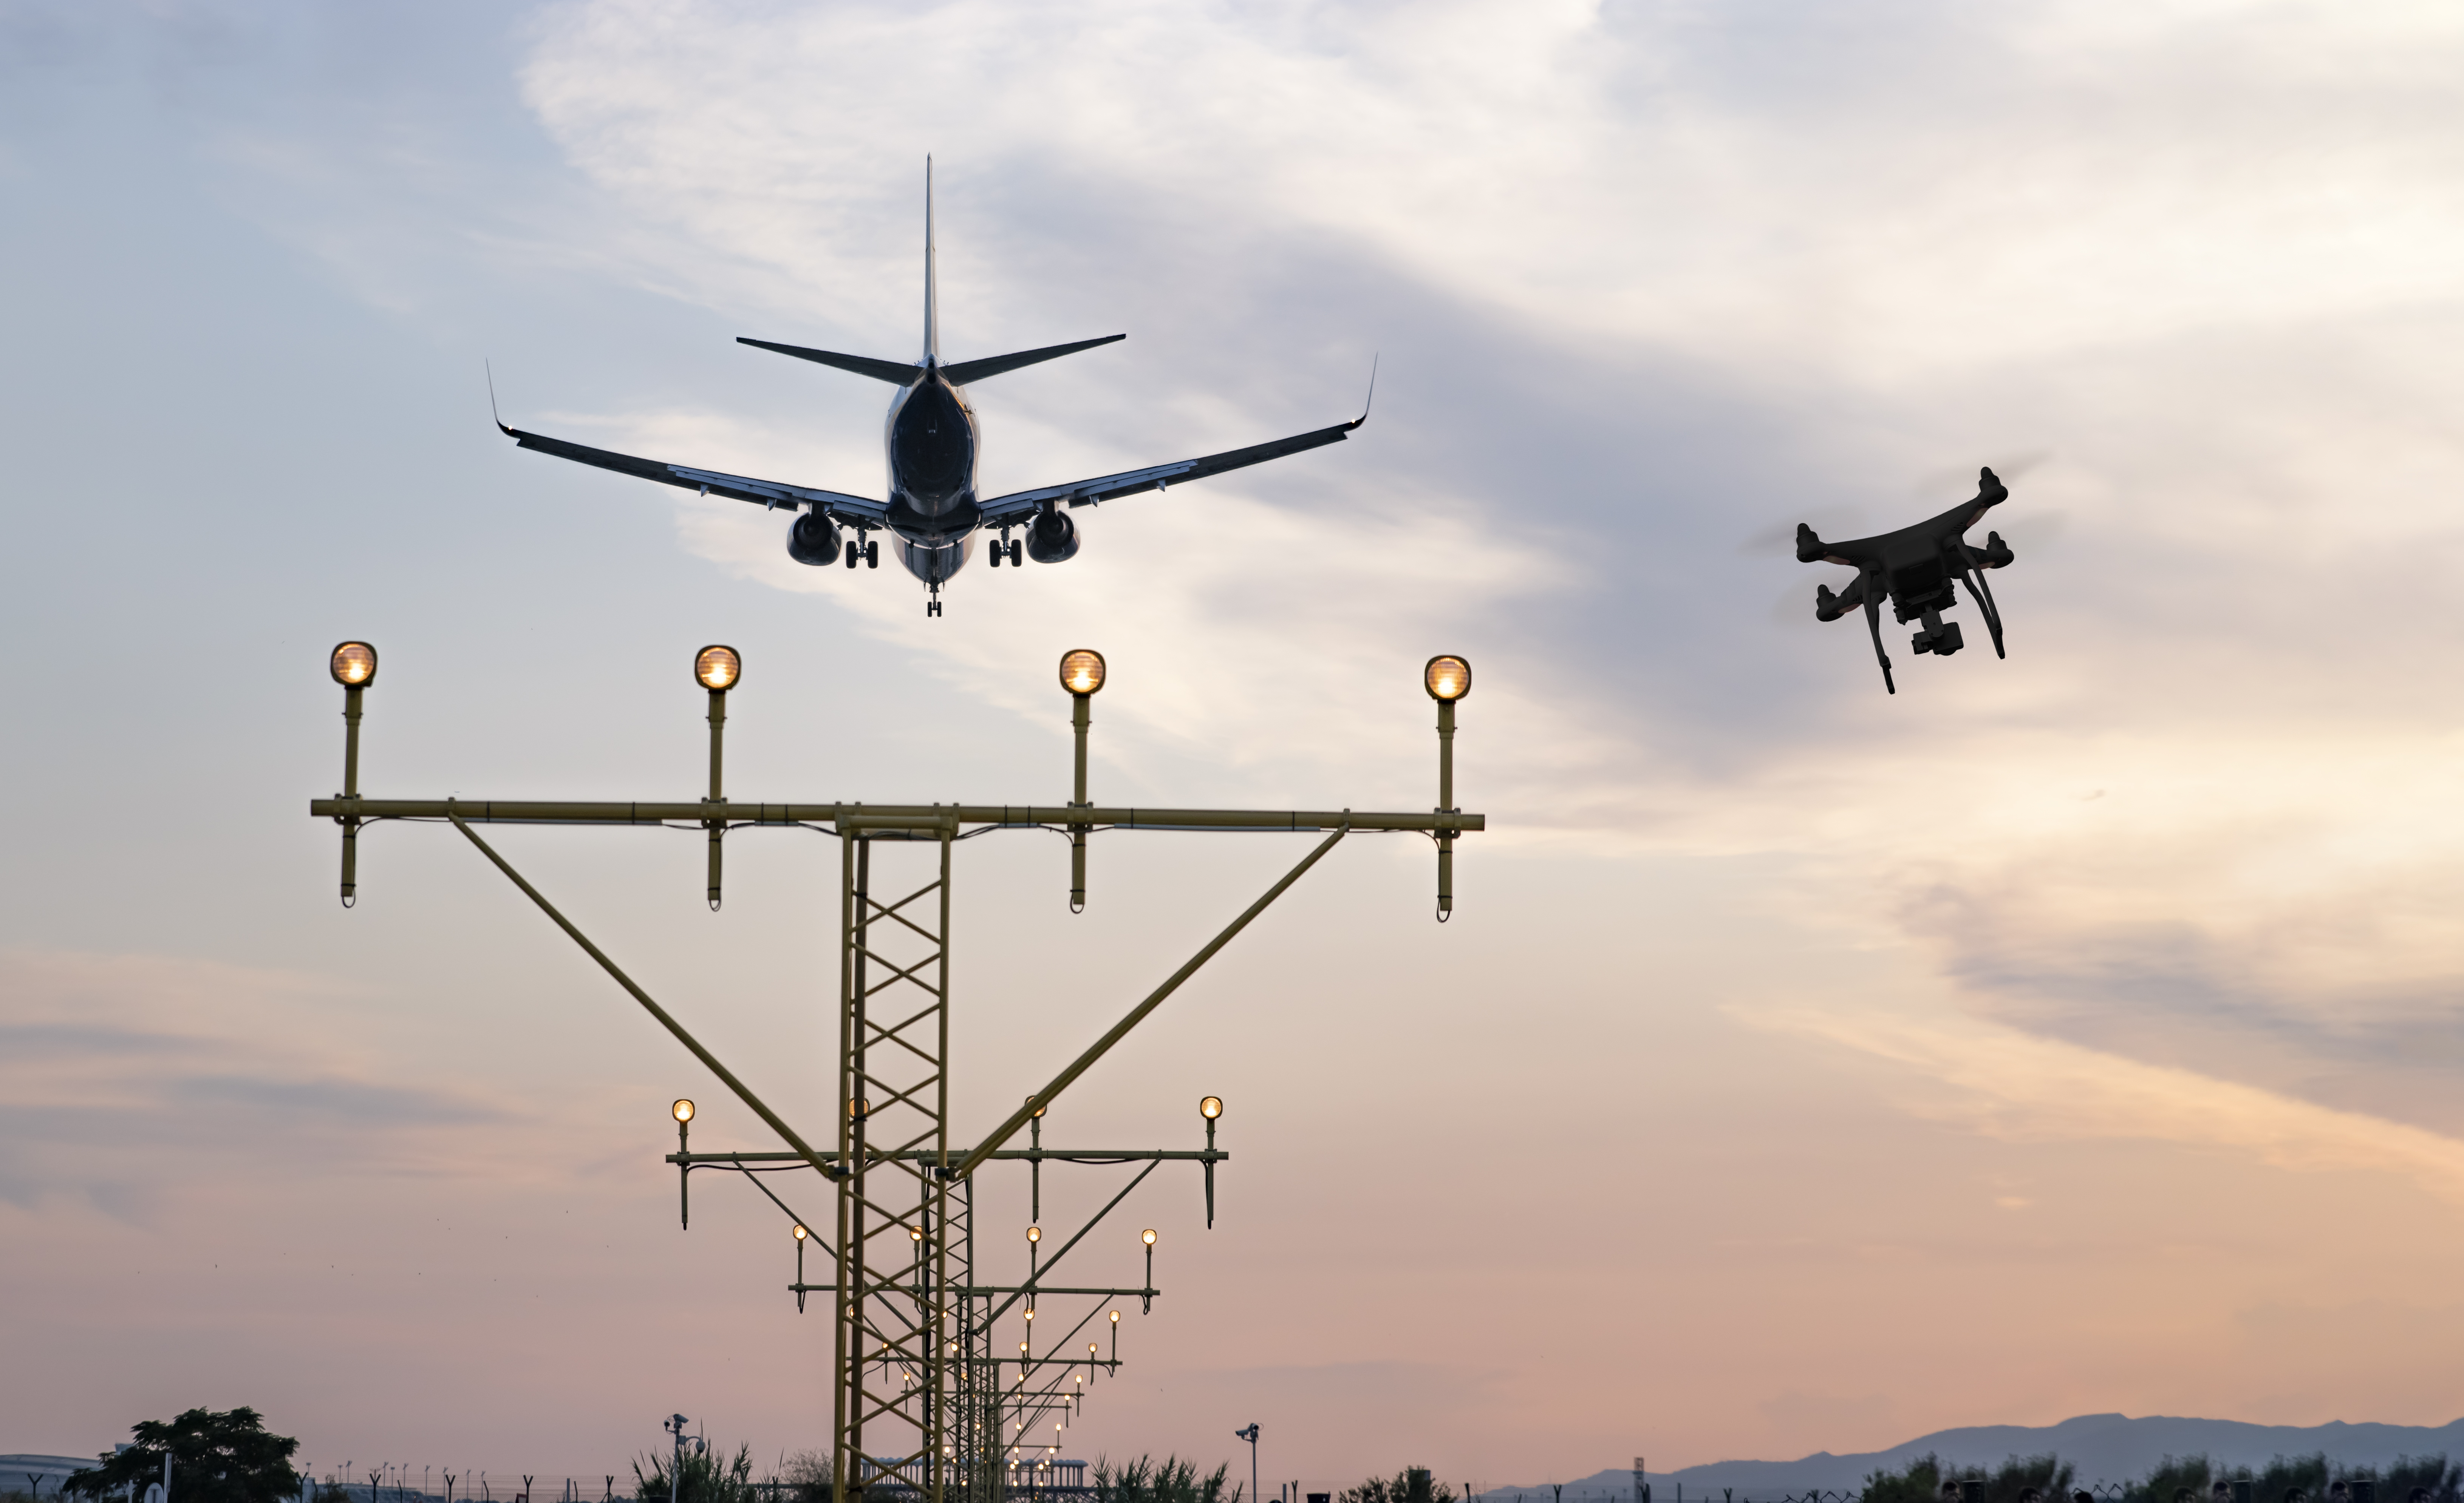
\includegraphics[width=10cm]{imgs/drone_with_plane_landing.jpg}
    \caption{Unauthorized drone near airport.}
\end{figure}




\section{Operational environment}
Great importance is given to the analysis of the context in which detection intends to operate. It is necessary to take into consideration the possible presence of other systems operating in RF and wireless communications like RFID, cellular network, wireless sensors network which can cause serious problems in the detection instruments. It is possible to refer to this type of environment with 'radiowave environment'. It is very important to choose carefully where to position the operational frequencies within it, in order to not cause interference to nearby systems and at the same time to respect the spectrum regulations that vary from region to region. Among all possible detection solutions for drone defense systems investigated by this thesis the primary one is the radar detection solution. In the figure \ref{specrtum} the frequency spectrum of interest is shown.

\begin{figure}[h!]
    \centering
    \includegraphics[width=13cm]{imgs/ElecSpect.jpg}
    \caption{Electromagnetic spectrum.}
    \label{specrtum}
\end{figure}

Considering the dimensions of drones that are in the range of centimeters, the frequencies need to detect this devices belong to the X, Ka, K, Ku bands. This range goes from 8 to 40 GHz and is a direct consequence of relationship between wavelength and frequency: $\lambda = c/f$. In fact, wavelengths of 1 cm - 10 cm correspond to this range of frequencies.
The current cellular bands are all in sub GHz range of spectrum and don't cause interference to our bands while several bands of 5G cellular network are in the range of frequencies considered and can interfere with the detection system. \\ Another important analysis to be carried out on the context is the physical one, named for simplicity "physical environment". It is possible to identify the physical characteristics of the context in which one intends to operate, characterized by the presence of people, obstacles, multipaths and blind areas that for example can cause a false detection or block the radar waveform. Having defined the two main components that make up the environment, let's now see what are the contexts in which we want to investigate the use of radar technology for drone detection. In general, in relation to the level of risk and the size of the area there are different specific needs for radar technologies and different costs. In a situation of high risk and very large area such as in the case of an airport or an oil refinery, it is not necessary to spare expenses and complexity. As a result, complex military-level solutions are accepted. On the other hand, civil situations characterized by a low budget and the presence of people in the vicinity of detection instruments, in some cases characterized also by a limited temporary duration (event), do not allow the use of military-level and/or fixed solutions. Consequently, in situations such as public events, squares full of people, perimeter areas (homes, prisons, stadiums) it is necessary to adopt solutions characterized by a lower complexity, a lower cost and simplicity of use and installation, all attributes contrary to the military field. \\ Figure \ref{context} shows a general grouping of the situations considered, the main discriminating factor among the contexts is the military and civil attribute. Subsequently it is possible to further subdivide the civil scenario into fixed and mobile solutions. The scenario investigated by the thesis concerns the civil context and all its sub-cases. These contexts are in general small and medium-sized areas such as individual homes, squares and perimeter areas like power plants, prisons, etc. It is necessary to pay attention to the radiowave environment, for example in case of a massive presence of people whereas each of them generally owns a smartphone that can operate in 5G bands and can cause problem to detection radar. For what concern the fixed solution in a civilian context it is easier to imagine a low cost fixed radar, while a real challenge is to be able to create a portable and low cost radar solution. An example for the latter case could be a radar used to protect the confidentiality and privacy of a very limited area, such as the case of a boat. 

\begin{figure}[h!]
    \centering
    \includegraphics[width=13cm]{imgs/Contexts groups.png}
    \caption{Context division.}
    \label{context}
\end{figure}

\newpage
\section{Detection technologies \cite{survey}}
Measurements by means of a radar are not the only ones possible to determine the presence of a drone in the surrounding area. During its flight, a drone can emit several types of measurable quantities such as:
\begin{itemize}
     \item Noisy sound,
         
    \item Heat,
        
    \item Radio frequency signals,
\end{itemize}

Consequently, it is possible to determine its presence by taking one or more of these measurements by the relative instruments that are IR/Optic cameras, acoustic sensors and radio frequency scanners. For the pros and cons of each technique an hybrid solution is preferable, in such a way that where a sensor has a gap it is filled by the other sensor. The radar solution is usually the most used due to the benefits of independence, privacy and performance and in many cases it not need other sensors because is the most complete solution. It follows a brief description of acoustic, thermal and radio frequency solutions. \\ Acoustic sensors are generally array of microphones, that are characterized by very low cost and small dimensions. On the other side this solution is strongly influenced by the presence of all background noises that cause a high alarm false rate. Considering also the short range offered, that is of hundreds of meters, the solution in question is not very useful. Example of use of this technique combined with machine learning achieve 83\% of accuracy and combined with k-nearest neighbors algorithm achieve 61\% of accuracy \cite{survey} \cite{robinradar1}. Unfortunately is not possible to retrieve direction of arrival of sound and perform tracking of drones. Thermal detection technologies allow to measure the heat emitted by the drone by means of infrared or optic cameras. In fact drone's components like motors, battery and hardware produce a significant amount of heat. Usually the measured data is compared with the characteristic IR signature of the drones, as happens for the remote sensing performed in satellite images. Each materials and objects have a characteristic reflectance of the light in a specific portion of spectrum that is a kind of signature. It is possible to use a convolutional neural network to process the thermal images to recognize the spectral signature and identify the possible presence of a drone \cite{survey}. This technique returns excellent results at a very low price but in practice the viewing range does not exceed one hundred meters and in public place there is also the problem of privacy if we consider the presence of cameras. Furthermore, this method is strongly influenced by atmospheric conditions. For all these reasons it can only be used together with other technologies such as radar. For example with a combination of radar and IR camera, the minimum radar detection range problem can be solved. Concerning radio frequency analyzers, they are devices capable of picking up micro waves and analyzing their spectrum. They can be exploited for the benefit of drone detection by intercepting messages exchanged between the drone and the controller. In the context of electronic warfare, this practice falls within the group of action called SIGINT or COMINT that stands for Signal Intelligence or Communication Intelligence. The use of these techniques deserves particular attention as commercial drones are often controlled by a remote pilot and the communication protocols between the drone and the controller are widely known. Therefore this knowledge can be fully exploited to recognize the drone model and undertake hijacking techniques. For example, if the message formats used between the controller and the drone are known, it is possible to create false messages and hijack the drone elsewhere without causing it to fall. Take the drone out from defended area without causing its crash, that can be a very dangerous event, is one of the most effective solution. Using this technique, the position of the drone is obtained from the information that it itself sends to the controller, as happens with the well-known air traffic system ADS-B. Therefore this technique is a dependent type solution, because it depend from the information sent by the drone, and for this reason it cannot be used as the only detection solution: if the drone is in autonomous flying mode or if the communication protocol of the messages exchanged with the controller is not known, it is impossible to detect it. Usually considering the extreme simplicity of implementation of these systems and their low cost, they are widely used and are often chosen as a drone detection solution together with a radar technology. With a solution of this type is also possible to localize a drone also if it doesn't communicate the information of location to their controller. For example, by using multiple RF receivers and by applying a type of multilateration technique \cite{survey}. It is important to clarify that also in this case is necessary to know the messaging protocol. Another possible use of RF scanner technique is within a neural network that perform the operation of classification of stolen signals \cite{survey}. So the advantages of a RF scanners are the low cost, the possibility to localize the drone also with multilateration technique and simplicity of implementation. On the other side a reasonable cons is the impossibility to detect drone in autonomous flight mode and that use a unknown protocol of messages. Current manufacturers of anti-drone technologies, to avoid blind spots, implement multiple detection systems with sensor fusion technology. A typical example of radar plus EO/IR sensor camera is shown in figure \ref{EOcamera}. This is one of the most complementary solution for drone detection because is possible to identify a threat seen by the radar at long distance by means of the EO/IR scanner that confirm or refuse the detection from radar. In this way the short range problem of EO/IR scanner is resolved by the radar and the low accuracy or identification problem of radar is resolved with the EO/IR scanner. So, also in the most part of commercial implementations the radar is seen as the main technology to detect  a drone and other sensors can be used together to achieve accuracy improvement.
\begin{figure}[h!]
    \centering
    \includegraphics[width=9cm]{imgs/radar + eo camera.jpg}
    \caption{Radar + EO scanner configuration.}
    \label{EOcamera}
\end{figure}

Another detection configuration, that does not involve the use of radar, could be the multiple RF sensors, which by combining the intercepted information between them is possible to locate and to track a target drone. An example is shown in the next figure.

\begin{figure}[h!]
    \centering
    \includegraphics[width=6cm]{imgs/RF scanner triangulation.png}
    \caption{RF scanners triangulation \cite{survey}.}
\end{figure}
\newpage

Even if the drones does not exchange information about its location, it's possible to locate it by measuring the time of arrival of messages at each RF receiver. But it is necessary that the intercepted radio frequency messages are with certainty associated with a drone present in the area. Obviously with this configuration it is not possible to identify a drone that does not exchange messages of any kind or whose message exchange method is unknown. Another hybrid combination is possible by means of radar plus acoustic sensors, that is another accuracy improvement for the radar solution. In table \ref{tab:Hybrid_solutions} are shown the hybrid solution proposed by the vendors and their range performance.
\\

\begin{table}[!h]
\begin{tabular}{|
>{\columncolor[HTML]{FFFFFF}}l |
>{\columncolor[HTML]{FFFFFF}}l |
>{\columncolor[HTML]{FFFFFF}}l |}
\hline
{\color[HTML]{000000} \textbf{Vendor, Model}}    & {\color[HTML]{000000} \textbf{Combined techniques}}           & {\color[HTML]{000000} \textbf{Range}} \\ \hline
{\color[HTML]{000000} ELTA, Droneguard}          & {\color[HTML]{000000} Radar + RF scanner + Camera}            & {\color[HTML]{000000} 4.5 km}         \\ \hline
{\color[HTML]{000000} Aaronia, AARTOS DDS}       & {\color[HTML]{000000} Radar + Camera}                         & {\color[HTML]{000000} 5 km}           \\ \hline
{\color[HTML]{000000} APS, Ctrl+sky}             & {\color[HTML]{000000} Radar + RF scanner + Camera + Acoustic} & {\color[HTML]{000000} 3 km}           \\ \hline
{\color[HTML]{000000} Cerbari}                   & {\color[HTML]{000000} RF scanner  + camera}                   & {\color[HTML]{000000} 3 km}           \\ \hline
{\color[HTML]{000000} Rodhe e Schwartz, Adronis} & {\color[HTML]{000000} RF scanner}                             & {\color[HTML]{000000} 3 km}           \\ \hline
{\color[HTML]{000000} Droneshield, Sentinel}     & {\color[HTML]{000000} Radar + RF scanner + Camera + Acoustic} & {\color[HTML]{000000} 3.5 km}         \\ \hline
\end{tabular}
\caption{Hybrid solutions \cite{survey}.}
\label{tab:Hybrid_solutions}
\end{table}

%\begin{figure}[h!]
 %   \centering
 %   \includegraphics[width=16cm]{imgs/Tabella hybrid.png}
 %   \caption{Hybrid solutions}
%\end{figure}





\clearpage

\section{Complete anti drone system}
A complete anti drone system must be able to perform all the actions necessary to block a drone, all the phases that the system must do are:
\begin{itemize}
     \item Detection phase;
         
    \item Identification phase;
        
    \item Neutralization phase.
\end{itemize}
It is important to clarify the different phases that an anti-drone system must carry out. In particular, considering the detection process, which we are interested in, it must necessarily also include a primary identification phase. This task is only to verify that detected object is a drone, while the next identification phase is necessary to distinguish between friend or foe drone and to evaluate the level of risk associated to it. For example, a drone can be easily confused with a bird or any other flying object. Consider that many hybrid solutions include a low-cost radar, it does not also implement the functionality to distinguish them which is instead delegated to another component as we have seen in the case of a radar plus EO/IR sensor configuration. On the other hand, there are more expensive radars that are able also to carry out the primary identification phase and therefore they can distinguish a drone from an object of the same size. For example, this operation can be done through spectral analysis, identifying the presence of rotating blades \cite{robinradar2}. It's important to to underline that this primary identification phase belongs to the detection phase and it is different from the next one identification which constitutes a completely separate phase. This is the task of understanding if the detected drone is a threat or not. In practice the result of this phase is to respond to the question: 'Is necessary to neutralize the detected drone?'. In a first experimental implementation based only on detection phase, we can simply assume that the area to be monitored does not admit the presence of any type of drone, friend or foe. In a more advanced implementation, however, it is possible to consider the presence of friendly drones and enemy drones and therefore we need to find a way to distinguish them. This task can have different solutions, for example a friend or foe style RFID technique can be used. In this case distance and speed are challenges since velocity can be very high and range must be very short. Another solution can be to track and then analyze the path of the drone by means of machine learning and neural networks. In this way is also possible to predict the drone's action and recognize a friend drone. This type of technique is the most suitable for a radar system because, unlike the RFID solution, it is also of independent type and don't need external information in addition to those provided by the radar. Another possible solution, dependent like RFID technique, is to adapt the ADS-B or FLARM system to drones \cite{survey}. The main difficult is the dimension of ADS-B module, but uAvionix propose the Ping2020 that is a family drone-ADS-B. The main limitation in this case is the price  that is very high. FLARM is less expensive solution primarily designed for light weight UAS (Unmanned Aerial Veichle) but it's encryption protocol add extra processing time and it is proprietary. \\
Once the drone is detected and confirmed as a threat can be very useful to estimate the level of risk associated to it. To do this is possible to implement a math model that associate a numerical risk value to the threat. For example a math equation like this can be used: 
$R=\left(R_{\text {object }}+R_{\text {path }}\right)^{R_{\text {time }}}$
\cite{survey}.

In general is necessary to classify the different areas in the supervised zone in relation to their risk, as is done with the ICAO area classification. Then the first value of risk $R_{\text{object }}$ come from the mass and velocity of drone that express its kinetic energy. This information come from the detection phase where in relation to the drone dimension a mass can be deduced, while velocity is properly measured by means of the Doppler frequency. Then, at this value is added the risk $R_{\text{path}}$ related to the actual position of drone, directly proportional to the area classification risk. Also proportional to the direction of drone's path and distance to the other areas by means of weighted sum. A picture where the drone flight direction and different areas with different risk is shown in figure \ref{risk}. Finally $R_{\text{time }}$ is related to the response time of neutralizing system that are described below.

\begin{figure}[h!]
    \centering
    \includegraphics[width=12cm]{imgs/Risk model.png}
    \caption{Different risk area related to drone path.}
    \label{risk}
\end{figure}

%soluzioni di neutralizzazione
Once the threat has been identified and its level of danger assessed, action must be taken. So the last step of an anti drone system is the neutralization. In general is possible to distinguish two type of neutralization technique:
\begin{itemize}
     \item Destructive techniques: in which the use of weapons is accepted that cause the fall down and consequent destruction of the drone. So this is a type of military solution;
         
    \item Non destructive techniques: where the use of military weapons is not admitted and is not possible to cause the fall down of the drone, so it is the most addicted solution in a civilian environment where the people are close to the target drone;

\end{itemize}

One of the most desirable non destructive technique is the drone hijacking. This neutralization solution is the safer technique, in fact the unauthorized drone is moved out the supervised area in a safe way. In practice a defender operator take the control of unauthorized drone in two stage. During the first stage he cause the disconnection between the original controller and the drone, breaking the pairing between them. Then during the second phase the defender operator execute the pairing with the drone and so became the new controller \cite{survey}. It's important to note that this neutralization solution is possible only if the attachment procedure with the drone is fully known and if the drone is not in an autonomous flight mode. This technique includes hacking and spoofing practices. In the next picture is shown a representative scheme of this technique.

\begin{figure}[h!]
    \centering
    \includegraphics[width=10cm]{imgs/Drone hijacking.png}
    \caption{Hijacking technique.}
\end{figure}

Another possible solution of neutralization is the spoofing technique. Considering that most of the commercial drone have a GPS module and rely heavily on the information received from it, is possible to send them a fake GPS position in order to confuse them. This technique is possible also when the drone is not controlled by a remote operator and is in autonomous flight mode.
Another possibility is the geofencing technique that is already implemented in almost all commercial drones. In practice, relevant areas such as an airport are saved into a database that is a collection of all restricted area for drones. Then many commercial drones are also equipped with an autolanding module that prevents the invasion of restricted area by accessing the database of restriction and controlling them. Obviously by modifying the commercial drone and eliminating this module is very simple to evade this check. These are the most used techniques for the non destructive set in which we are interested. Then for completeness also few destructive  technique are listed below. Killer drones are called the practice of attack or damage of enemy drones by means of friend drone. Drone capture is instead the practice of capturing the unauthorized drone by means of net in a terrestrial or aerial way. Also the jamming can be considered as a destructive technique because it can cause the drone to fall. Is possible to distinguish different kind of jamming in relation to the direction, the position and the bandwidth of jammer. A very useful approach can be the GPS jamming because the GPS protocol is fully known instead the messaging protocol of the drone can be unknown. As mentioned above, however, jamming solutions are unusable in the civil field not only for the possibility of causing a fall but also for the regulation of the spectrum and interference to other telecommunication systems. While the other mentioned destructive techniques are not usable in a crowded context for the safety of people.
Another important consideration are done for better design a complete drone defense system. Considering the rapid evolution of drone technology, and the different instrument of detection used is necessary to design a modular system, in this way, each component can be updated and will help keep the system up-to-date.


%capitolo2
\chapter{Radar solutions}
%Caratteristiche principali delle misurazioni radar for drone detection, %benefici e contro.
%Esempi di implementazioni radar possibili, stato dell'arte %(caratteristiche robin, informazioni pi\'u complete) 


%1. Radar position in surveillance systems. Pros and cons of radar for drone detection.
%2. Requirements for drone detection, example of FMCW solution 
%3. State of the art for drone detection (analysis of current radar solution).
%4. Definizione architettura e dimensionamento radar for drone detection to achieve the desirable goal.

In this chapter the radar drone detection technology is analyzed. For a better understanding, a general introduction to radar technologies is made and then follows a brief description of an example of radar technology (FMCW radar) choice considering the radar requirements for drone detection. Then the state of the art of solutions currently on the market are analyzed. 
In the end by using a 'top-down' approach a possible architecture of radar for drone detection is defined and dimensioned. 

\section{Radar technology}
Radar is one of the most widely used surveillance technology as it allows to measure the shape, the distance, the speed and the direction of arrival of the received reflected signal. To better understand where the radar is among the surveillance systems, we can divide surveillance technologies into two large groups: 
\begin{itemize}
     \item \textbf{Cooperative surveillance}: contain all techniques that rely on target devices, are included all technologies that need the cooperation of target to detect it. Is also subdivided in two other groups, dependent and independent type. The dependent cooperative surveillance systems do not perform any type of measurement and can only read information received from targets. The independent cooperative surveillance systems need only that target can reply to the messages, and for example by measuring the ToA the ground sensors can calculate it's horizontal position. 
         
    \item \textbf{Non cooperative surveillance}: include all techniques of surveillance that do not rely on target reply or target cooperation during the process of localization.
        
\end{itemize}

Considering the principle of operation of a radar, is simple to understand that it belongs to the typology of independent surveillance technologies. Then considering the mobility of a radar it's possible to classify them in rotatory radar or fixed radar. The first solution is characterized by a continuous rotation in azimuth performed by mechanical movements. While with the fixed radar an array of antennas is used to electronically scan the area, so the beam steering is performed only by changing the phases of elements.
It is useful to classify radars according to the number of quantities they are able to measure, considering the electronic or mechanical rotation also.
We can distinguish respectively 2D,3D and 4D radars.
\begin{itemize}
     \item \textbf{2D}: These are typically the less expensive configurations that can be implemented without the use of a phased array antenna. Mainly, there is only a mechanical rotation that allows you to scan the surrounding area in azimuth. In this case two dimensions can be measured: the slant range and the azimuth direction of arrival. An additional radar is delegated to obtain the information about the elevation of target, if needed.
         
    \item \textbf{3D}: With the use of phased array antennas technology, it is possible to combine mechanical azimuth scanning with vertical electronic scanning. This gives three dimensions that can be measured: the slant range, the azimuth arrival direction, and the elevation information.
    
    \item \textbf{4D}: In addition to the 3D measurements of distance, direction and vertical information this type of radar measures also the Doppler information. But also the 2D radar is capable to measure the Doppler information, so in general 4D is also a market name strategy. For simplicity we refer to a 4D radar as imaging radar or holographic radar that is able to reconstruct an image of observed situation. Usually these are used for automotive, in particular for driving assistance. The technology used is also the antenna phased array, both an horizontal and vertical array configuration. In this case the processing of received data is interested in electromagnetic pattern of received signal. A machine learning technique can be used to recognize the pattern of signals. The maximum range achievable with this technology is not too long, we are talking about several hundreds of meters.

\end{itemize}

Focusing on phased array antenna technology, two main implementations can be distinguished:

\begin{itemize}
     \item \textbf{PESA}: Passive Electronic Scanning Array is the configuration with a single transmitter/receiver linked to all the antenna elements by means of a phase shifter. In this way the only result achievable is the steering of the beam because only one single beam at one single frequency can be transmitted at time.

         
    \item \textbf{AESA}: Active Electronic Scanning Array is the configuration in which there are several transmitter/receiver, one for each element. In this way more complex action can be performed, for example more simultaneous beams at different frequency can be transmitted.
        
\end{itemize}



\begin{figure}
    \centering
    \subfloat[PESA]{{\includegraphics[width=10cm]{imgs/PESA radar.png} }}
    \qquad
    \subfloat[AESA]{{\includegraphics[width=10cm]{imgs/EASA radar.png} }}
    \caption{PESA vs AESA configurations.}
\end{figure}


In general, the configuration with vertically and horizontally arranged arrays (4D radars) used in conjunction with an FMCW technology is a promising solution for the drone detection case. \\ Another possible implementation of low cost radars is that of passive radars, PR. Exploiting the possible presence of the so-called Illuminators of Opportunity (IoP), in this way the presence of transmitters is completely eliminated, the architecture of the radar is greatly simplified and costs are also reduced. In this way the detection is completely based on the presence of radio signals transmitted by third party devices, such as digital television (DVB-T) and consequently it is not possible to design an appropriate waveform and cover contexts in which third party illuminators are not available.\\
Among the mentioned radar technologies, those that are of most interest for the application of drone detection are those with low cost, considering the treated context. Regarding the benefits and cons of the drone detection radar solution, early drone detection systems initially did not rely on radar technology due to the extremely low RCS of drones. Considering also that radar are primarily designed for bigger object like in the case of Primary Surveillance Radar. The main benefits of using a radar solution, as described in \cite{robinradar} are:
the large detection range in contrast with the range of the others solution precedent depicted. The constant tracking, that is a practice very advanced with radar which also enable the multiple targets tracking simultaneously. The possibility to track autonomous flying drones, which RF solution are not able to detect. The independence from weather conditions, which affect most of the previously seen solutions, such as IR/EO cameras. On the other hand the cons of this solution are: the detection range, in the end depends also on on the drone's dimensions, in fact it is directly proportional to RCS as is possible to understand by seeing the radar equation. The main difficulty is the distinction between a drone and any other flying object of the same size or a bird, in fact the classic radars are not able to distinguish them as in the case of PSR. The drone's small weight and their quickly acceleration make them possible to perform extreme maneuvering that make detection very difficult. Another cons is the band used and the related frequencies that are subject to regulation that varies from region to region. These must also be properly chosen to avoid interference as well. A brief summary of the pros and cons of the radar solution for drone detection is shown in the table \ref{tab:prosandcons}\\
\begin{table}[h!]
\centering
\begin{tabular}{|l|l|}
\hline
{\color[HTML]{000000} \textbf{Radar detection pro}}     & {\color[HTML]{000000} \textbf{Radar detection cons}}  \\ \hline
{\color[HTML]{000000} Long range detection}             & {\color[HTML]{000000} Low RCS drone}                \\ \hline
{\color[HTML]{000000} Drone autonomous flight}        & {\color[HTML]{000000} Distinction from birds}         \\ \hline
{\color[HTML]{000000} Constant tracking}                & {\color[HTML]{000000} Transmission frequency license} \\ \hline
{\color[HTML]{000000} Independence of visual condition} & {\color[HTML]{000000} Interference}                   \\ \hline
{\color[HTML]{000000} High accuracy localization}       & {\color[HTML]{000000} Low speed}                      \\ \hline
\end{tabular}
\caption{Pros and cons of drone's radar detection.}
\label{tab:prosandcons}
\end{table}

\newpage
%in seguito i benefici e i contro della soluzione radar for drone detection.
\section{Requirements and FMCW radar}
Having defined the operational environment and the features of drones in the previous chapter, a first analysis of the general requirements for a radar is made. The first two fundamental needs to reveal a drone concern the Radar Cross Section and the Doppler analysis. Since the dimensions of drones are very small, typical values of RCS are in the order of 0.01 - 0.03 square meters \cite{rcsdrone}. So, as mentioned in the previous chapter it's necessary that frequency belongs to bands that goes from 8 to 20 GHz. Concerning the velocity measurements, a continuous wave radar is able to measure the velocity using the Doppler information. Being interested in both distance and speed measurement a frequency modulated continuous wave radar (FMCW) is one of the possible solutions. Considering also that is necessary a further Doppler processing during the detection that help to distinguish moving target and solve the problem of primary identification. The measurement related to the detection must be processed by micro Doppler analysis and then compared to a model \cite{microdoppler_and_SVM}. This task requires additional time which is added to the standard time of detection, so unlike a PSR (Primary Surveillance Radar) in this case the detection time could be greater. So, one of the objective can be to reduce at the minimum the time of detection while keeping the level of accuracy acceptable.\\ Another important consideration is about the maximum power transmitted, considering the near presence of people, it must be not so high and it is another motivations to use a FMCW radar that is characterized by a low peak power. Thinking about the radar architecture, a monostatic configuration can be a useful solution considering the requirements of portability for public environment. In figure \ref{FMCWradarchain} a typical FMCW radar chain is shown. 

\begin{figure}[h!]
    \centering
    \includegraphics[width=13cm]{imgs/FMCW radar chain.png}
    \caption{FMCW radar chain.}
    \label{FMCWradarchain}
\end{figure}
In this configuration the isolation between transmission and reception antenna is not perfect so considering also the antenna mismatch  is possible to use a Reflected Power Canceller (RPC) in addition to the classical radar chain. 
It is possible to observe that the phase reference is maintained known and a coherent detector is used, then the reflected signals received is analyzed in the spectral domain and starting from frequency variations, velocity and distances are measured. To do this a Fast Fourier Transform is used. So the FMCW radar represents a possible candidate for the solution of the drone detection problem. It is therefore appropriate to better analyze its characteristics. The typical signal used by this type of radar is a chirp signal characterized by a linear change in frequency over time. In this way the reflected echo mixed with the transmitted signal will produce a frequency difference called beat frequency and knowing the time-relation of this frequency is possible to obtain the range and velocity quantities. It's possible to demonstrate that higher the bandwidth means higher the range resolution. On the other hand, by increasing the modulation period at equal bandwidth means a lower frequency to measure and an higher frequency resolution. An example of linear frequency modulation is shown below. 

\begin{figure}[h!]
    \centering
    \includegraphics[width=8cm]{imgs/Fmcw modulation.png}
    \caption{FMCW modulation}
\end{figure}

The advantages of FMCW radar respect to a classic pulsed radar are:

\begin{itemize}

    \item \textbf{Low peak power}: there is no standby period and so the transmitted power is linearly spreaded among the channel, this means also a low probability of intercept; 
         
    \item \textbf{Higher bandwidth}: its possible to demonstrate that higher the bandwidth of modulation means higher the range resolution; 
    
    \item \textbf{Short-range detection}, no blind spot in front of the radar because there is continuous transmission and reception unlike a pulsed radar;

    \item \textbf{Low cost receiver}, because IF bandwidth related to sampling frequency is minor than total bandwidth of  chirp;
    
    \item \textbf{Radar dimensions}, typical implementations of this radar are very small and give the possibility to create a radar through off the shelf components ;
        
\end{itemize}

\section{State of the art for radar drone detection system}
Follow a brief description of current solutions that it's possible to find on the market, but most of these solutions are either of military level and/or expensive. 
\subsection{Robin Radar, Elvira and Iris}
Some solutions offered by Robin Radar make use of FMCW radar technology.  In particular, two solutions are offered, respectively called IRIS and ELVIRA, the first more expensive 3D type and the second less expensive 2D type. The radars in question are capable of doing tracking, multi target detection and micro Doppler analysis. In addition, the lightest solution in this case comes to weigh 25 kg and has dimensions of 55x62 cm. So it is also considerable as portable solution but it's possible to find lighter and smaller solutions for extreme portability needs. As can be seen from the specifications shown in the table \ref{tab:robinradar}, the technique used to distinguish a drone from another object or bird is that of micro Doppler analysis.

\begin{table}[h!]
\centering
\begin{tabular}{|
>{\columncolor[HTML]{FFFFFF}}l |
>{\columncolor[HTML]{FFFFFF}}l |
>{\columncolor[HTML]{FFFFFF}}l |}
\hline
{\color[HTML]{000000} \textbf{SPEC}}         & {\color[HTML]{000000} \textbf{IRIS}}          & {\color[HTML]{000000} \textbf{ELVIRA}}        \\ \hline
{\color[HTML]{000000} Technology}            & {\color[HTML]{000000} FMCW}                   & {\color[HTML]{000000} FMCW}                   \\ \hline
{\color[HTML]{000000} Frequency}             & {\color[HTML]{000000} X-Band (8900-9650 MHz)} & {\color[HTML]{000000} X-Band (8700-9650 MHz)} \\ \hline
{\color[HTML]{000000} Power Output}          & {\color[HTML]{000000} 2 x 12 Watt}            & {\color[HTML]{000000} 4 Watt}                 \\ \hline
{\color[HTML]{000000} Instrument Range}      & {\color[HTML]{000000} 5 km}                   & {\color[HTML]{000000} 5 km}                   \\ \hline
{\color[HTML]{000000} Detection Range}       & {\color[HTML]{000000} 4 km}                   & {\color[HTML]{000000} 2.7 km}                 \\ \hline
{\color[HTML]{000000} Classification Range}  & {\color[HTML]{000000} 2.2 km}                 & {\color[HTML]{000000} 1.8 km}                 \\ \hline
{\color[HTML]{000000} Main Beam Width}       & {\color[HTML]{000000} 6\degree x 60\degree}             & {\color[HTML]{000000} 10\degree x 10\degree}            \\ \hline
{\color[HTML]{000000} Rotation}              & {\color[HTML]{000000} 30 rpm}                 & {\color[HTML]{000000} 46 rpm}                 \\ \hline
{\color[HTML]{000000} Classification Method} & {\color[HTML]{000000} Micro-Doppler}          & {\color[HTML]{000000} Micro-Doppler}          \\ \hline
{\color[HTML]{000000} Range Accuracy}        & {\color[HTML]{000000} 0.6 m}                  & {\color[HTML]{000000} 0.6 m}                  \\ \hline
{\color[HTML]{000000} Azimuth Accuracy}      & {\color[HTML]{000000} 0.6\degree}                  & {\color[HTML]{000000} 1\degree}                    \\ \hline
\end{tabular}
\caption{Robin radar specification.}
\label{tab:robinradar}
\end{table}
\newpage
For what concern the 3D solution, the maximum range in which a drone the size of a DJI Inspire can be detected is 4 km. In contrast, the maximum range within which a drone can be classified and distinguished from a bird is only 2.2 km. In this case, the configuration used for the antenna is a linear array type. As it is possible to observe in figure \ref{irisimg} there are four rotating arrays (30 rpm). In fact, counting the number of elements that make up each array and considering the frequency used, it is possible to calculate the width of the beam in elevation. If we consider that each element is placed at $\lambda/2$  and each has a width of about 1 cm, the width of the beam is about 6\degree.

\begin{figure}[h!]
    \centering
    \includegraphics[width=8cm]{imgs/IRIS robin.png}
    \caption{IRIS arrays configuration.}
    \label{irisimg}
\end{figure}

For what concern the 2D radar a heavier solution has been considered, of about 75 kg. Consequently, this configuration makes this solution less suitable for extreme portability situation. On the other hand, in this case there is a much lower power consumption and the detection range is 1.3 km smaller than the 3D configuration. Also the width of the main beam in azimuth is smaller than in the previous case, it is equal to 10 degrees both in azimuth and in elevation. In fact is necessary a rotation velocity of 45 rpm to achieve a good result of accuracy in front of a reduced beamwidth. 

\subsection{Aveillant, Gamekeeper 16U}
Another interesting solution is that offered by Aveillant, which specializes in holographic radar design. The technology used here deviates greatly from the simple linear arrays just seen and is based on the technology previously mentioned as 4D radar. The goal is to reconstruct a 3D image of the surrounding environment based on the pattern waveform information collected at the radar. This solution is not addicted for portable needs, in fact the weight is about 370 kg and dimensions are 3.5 m x 0.95 m x 0.4 m. Considering also the high power consumption is not considered as a low cost solution. The specifications and performance are shown below.

\begin{table}[h!]
\centering
\begin{tabular}{|
>{\columncolor[HTML]{FFFFFF}}l |
>{\columncolor[HTML]{FFFFFF}}l |}
\hline
{\color[HTML]{000000} \textbf{SPEC}}      & {\color[HTML]{000000} \textbf{Gamekeeper 16U}}   \\ \hline
{\color[HTML]{000000} Technology}         & {\color[HTML]{000000} Holographic radar}         \\ \hline
{\color[HTML]{000000} Frequency}          & {\color[HTML]{000000} L-Band}                    \\ \hline
{\color[HTML]{000000} Power Output}       & {\color[HTML]{000000} 2 kW}                      \\ \hline
{\color[HTML]{000000} Instrument Range}   & {\color[HTML]{000000} 7.5 km}                    \\ \hline
{\color[HTML]{000000} Detection Range}    & {\color[HTML]{000000} 5 km}                      \\ \hline
{\color[HTML]{000000} Target RCS}         & {\color[HTML]{000000} 0.01 m\textasciicircum{}2} \\ \hline
{\color[HTML]{000000} Range in Altitude}  & {\color[HTML]{000000} 900 m}                     \\ \hline
{\color[HTML]{000000} Azimuth Coverage}   & {\color[HTML]{000000} 90\degree}                      \\ \hline
{\color[HTML]{000000} Elevation Coverage} & {\color[HTML]{000000} 30\degree}                      \\ \hline
{\color[HTML]{000000} Range Accuracy}     & {\color[HTML]{000000} 0.6 m}                     \\ \hline
{\color[HTML]{000000} Azimuth Accuracy}   & {\color[HTML]{000000} 0.6\degree}                     \\ \hline
\end{tabular}
\caption{Gamekepeer 16U specifications.}
\label{tab:gamekeeper}
\end{table}

\begin{figure}[h!]
    \centering
    \includegraphics[width=6cm]{imgs/Gamekeeper 16U.png}
    \caption{Gamekeeper 16U.}
    \label{gamekeeperimg}
    
\end{figure}


To better understand how this radar work is necessary to explain the holographic principle on which it is based, discover by Gabor in 1948 \cite{holographic}. Both the spatial and temporal information of an electromagnetic wave are imprinted in the phase. In fact, it is possible to express it as: $\phi=\omega t+\boldsymbol{k} \boldsymbol{z}+\phi_{0}$
Unfortunately, it is not possible to save directly the visible light phase in any way, due to the higher frequency (hundreds of THz). Holograms are just used for this, thanks to an interference they can record the phase information. Using a reference wave, the interference that occurs between the echo reflected by the target and that of the reference wave is imprinted on a film. Then, the film is illuminated with the reference wave and thanks to the phenomenon of diffraction is produced a mirror wave to that reflected by the target. The same principle is reproduced with radars where the film surface is seen like a receiver array where each element can calculate the phase difference between a reference wave and a received wave. For example, is possible to use a power splitter to divide the 'reference wave', that remains in radar and is used to demodulate the received signal and the 'illuminated wave', that is amplified and radiated by the antenna. In this case the interference between the echo signal and the reference wave took place in the demodulator instead of a metallic film. This mode of operation is very similar to that used by an FMCW radar, where the transmitted and received signals are mixed together and the result is a signal at a beat frequency.

\subsection{Kelvin Hughes, Spexer360}
Regarding other radar technologies, is possible also to identify the one offered by Kelvin Hughes that is based on a solid-state pulse radar. The technology is based on Sharp Eye, a class of radars developed by the same company, the main feature of this radar is the compactness, thanks to the small size is easily deployable and can be carried by a man on foot. Usually is combined with electro optic cameras to achieve high performance against drones. To achieve a good result in detect small aerial vehicle is crucial the post processing, are implemented the pulse compression, the Doppler analysis and the adaptive clutter suppression techniques. The dimension of rotating antenna is of 522 mm. Follow a recap of specification available of this solution (table \ref{spexerspec}).

\begin{table}[h!]
\centering
\begin{tabular}{|
>{\columncolor[HTML]{FFFFFF}}l |
>{\columncolor[HTML]{FFFFFF}}l |}
\hline
{\color[HTML]{000000} \textbf{SPEC}}        & {\color[HTML]{000000} \textbf{Spexer 360}}        \\ \hline
{\color[HTML]{000000} Technology}           & {\color[HTML]{000000} Solid State Pulse Radar}    \\ \hline
{\color[HTML]{000000} Frequency}            & {\color[HTML]{000000} X-Band {[}9.22-9.38 GHz{]}} \\ \hline
{\color[HTML]{000000} Power Output}         & {\color[HTML]{000000} 80 W}                       \\ \hline
{\color[HTML]{000000} Instrument Range}     & {\color[HTML]{000000} 2.4 km}                     \\ \hline
{\color[HTML]{000000} Target RCS}           & {\color[HTML]{000000} 0.03 m\textasciicircum{}2}  \\ \hline
{\color[HTML]{000000} Range accuracy}       & {\color[HTML]{000000} 5 m  RMS}                   \\ \hline
{\color[HTML]{000000} Azimuth accuracy}     & {\color[HTML]{000000} 0.8\degree  RMS}                 \\ \hline
{\color[HTML]{000000} Azimuth Beam Width}   & {\color[HTML]{000000} \textless{}4.0\degree}            \\ \hline
{\color[HTML]{000000} Elevation Beam Width} & {\color[HTML]{000000} 25\degree}                       \\ \hline
{\color[HTML]{000000} Range Accuracy}       & {\color[HTML]{000000} 0.6 m}                      \\ \hline
{\color[HTML]{000000} Azimuth Accuracy}     & {\color[HTML]{000000} 0.6\degree}                      \\ \hline
\end{tabular}
\caption{Spexer360 specifications.}
\label{spexerspec}
\end{table}

In figure \ref{spexerimg} is shown a typical installation with electro optic cameras.

\begin{figure}[h!]
    \centering
    \includegraphics[width=4cm]{imgs/Kelvin hughes .png}
    \caption{Spexer 360 installation.}
    \label{spexerimg}
\end{figure}
\newpage
\subsection{Droneshield, RadarZero}
One of the solutions closest to the needs of our cause is that offered by the company Droneshield, called RadarZero. This company is specialized in drone detection and contrast solutions, they have also produced a wearable RF detector that is completely passive and weighs only 700 g, addicted to military environments it is able to detect a cooperating drone. The RadarZero is the most compact solution observed so far, as big as a notebook (20 cm x 16 xm x 5.6 cm). Moreover, it provides a relaxed range constraint of about maximum 1 km as detection range. It seems to be the most promising solution considering the ease of transport, use, installation and cost. In fact, it does not seem to be a solution designed for military cases, but it is perfectly suited to civilian and private contexts. It has been successfully demonstrated with the TIPS-C (Trakka Interceptor Package Solution) system at Eglin Air Force Base. In figure \ref{radarzero} is shown the typical installation of RadarZero, in this case is possible to observe four module each one covering 90 degrees, and other optical system. The interesting fact is that it requires no initial calibration and transmits very low power.

\begin{figure}[h!]
    \centering
    \includegraphics[width=8cm]{imgs/RadarZero installation.png}
    \caption{RadarZero installation.}
    \label{radarzero}
\end{figure}

\newpage


\begin{table}[]
\centering
\begin{tabular}{|
>{\columncolor[HTML]{FFFFFF}}l |
>{\columncolor[HTML]{FFFFFF}}l |}
\hline
{\color[HTML]{000000} \textbf{SPEC}}      & {\color[HTML]{000000} \textbf{Droneshield Radar Zero}} \\ \hline
{\color[HTML]{000000} Technology}         & {\color[HTML]{000000} -}                               \\ \hline
{\color[HTML]{000000} Frequency}          & {\color[HTML]{000000} K band (24.45 - 24.65 GHz)}      \\ \hline
{\color[HTML]{000000} Power Output}       & {\color[HTML]{000000} 3.4 W}                           \\ \hline
{\color[HTML]{000000} Instrument Range}   & {\color[HTML]{000000} 1 km}                            \\ \hline
{\color[HTML]{000000} Target RCS}         & {\color[HTML]{000000} -}                               \\ \hline
{\color[HTML]{000000} Range in Altitude}  & {\color[HTML]{000000} -}                               \\ \hline
{\color[HTML]{000000} Azimuth Coverage}   & {\color[HTML]{000000} 80\degree}                             \\ \hline
{\color[HTML]{000000} Elevation Coverage} & {\color[HTML]{000000} 90\degree}                             \\ \hline
{\color[HTML]{000000} Azimuth Accuracy}   & {\color[HTML]{000000} 1\degree}                             \\ \hline
\end{tabular}
\caption{RadarZero specifications.}
\label{radarzerospec}
\end{table}

In table \ref{radarzerospec} the specifications available is shown.
Unfortunately, the information about the radar technology used by RadarZero is not know and is possible only to derive and suppose it.

\subsection{Advance Protection System, FIELDCtrl Access}
Advance Protection System (APSsystem), work in the protection of airspace and offers different solutions in the field of drone defense specialized in ultra precise 3D MIMO radars. They designed several radar solutions by gradually increasing performance and cost. The entry level and less expensive solution is the FIELDCtrl Access, with a detection range of 2 km and AESA e MIMO (Multiple Input Multiple Output) technology for antennas. A typical antennas configuration and radar housing is shown in figure \ref{CTRLantenna}.

\begin{figure}[h!]
    \centering
    \includegraphics[width=13cm]{imgs/Ctrl acces antenna.png}
    \caption{FIELDCtrl Antennas.}
    \label{CTRLantenna}
\end{figure}

Below are shown the specification of this configuration (table \ref{FIELDctrltab}), the results are more interested for our cause because the design and implementation of a  2D array patch antenna like this is very powerful and cheap thanks to the technological improvements in this field. On the other side, management and processing of information coming from MIMO configuration like this is very challenging and is the more expensive part. 
\begin{table}[h!]
\centering
\begin{tabular}{|
>{\columncolor[HTML]{FFFFFF}}l |
>{\columncolor[HTML]{FFFFFF}}l |}
\hline
{\color[HTML]{000000} \textbf{SPEC}}             & {\color[HTML]{000000} \textbf{FIELDctrl Access}} \\ \hline
{\color[HTML]{000000} Technology}                & {\color[HTML]{000000} 3D MIMO/AESA}              \\ \hline
{\color[HTML]{000000} Frequency}                 & {\color[HTML]{000000} X-Band}                    \\ \hline
{\color[HTML]{000000} Power Output}              & {\color[HTML]{000000} 2 kW}                      \\ \hline
{\color[HTML]{000000} Instrument Range}          & {\color[HTML]{000000} 7 km}                      \\ \hline
{\color[HTML]{000000} Detection Range}           & {\color[HTML]{000000} 2 km}                      \\ \hline
{\color[HTML]{000000} Target RCS}                & {\color[HTML]{000000} 0.01 m\textasciicircum{}2} \\ \hline
{\color[HTML]{000000} Range Accuracy/Resolution} & {\color[HTML]{000000} 10 m / 6 m}                \\ \hline
{\color[HTML]{000000} Azimuth Coverage}          & {\color[HTML]{000000} 90\degree}                      \\ \hline
{\color[HTML]{000000} Elevation Coverage}        & {\color[HTML]{000000} 45\degree}                      \\ \hline
\end{tabular}
\caption{FIELDctrl access specifications.}
\label{FIELDctrltab}
\end{table}

\subsection{ART, Midrange 3D}
Advanced Radar Technologies group, born as a spin off of the microwave and radar research group in Madrid (Universidad Politecnica de Madrid), is interested in the unmanned aircraft traffic management (UTM). They propose a FMCW technology with a rotating radar, midrange 3D achieve the better range distance in which a micro UAS of about 0.01 $m^2$ RCS is detectable, that is 3 km. In this case the weight is about 75 kg and for this is not so portable in some cases. Below are shown specification of this radar (table \ref{arttab}).

\begin{table}[h!]
\centering
\begin{tabular}{|
>{\columncolor[HTML]{FFFFFF}}l |
>{\columncolor[HTML]{FFFFFF}}l |}
\hline
{\color[HTML]{000000} \textbf{SPEC}}             & {\color[HTML]{000000} \textbf{ART midrange  3D}} \\ \hline
{\color[HTML]{000000} Technology}                & {\color[HTML]{000000} CWLFM}                     \\ \hline
{\color[HTML]{000000} Frequency}                 & {\color[HTML]{000000} Ku-Band {[}16 - 17 GHz{]}} \\ \hline
{\color[HTML]{000000} Power Output}              & {\color[HTML]{000000} 15 W}                      \\ \hline
{\color[HTML]{000000} Instrument Range}          & {\color[HTML]{000000} 10 km}                     \\ \hline
{\color[HTML]{000000} Detection Range}           & {\color[HTML]{000000} 3 km}                      \\ \hline
{\color[HTML]{000000} Target RCS}                & {\color[HTML]{000000} 0.01 m\textasciicircum{}2} \\ \hline
{\color[HTML]{000000} Range Accuracy/Resolution} & {\color[HTML]{000000} 0.25 m / 0.2 m}            \\ \hline
{\color[HTML]{000000} Azimuth Coverage}          & {\color[HTML]{000000} 360\degree}                     \\ \hline
{\color[HTML]{000000} Rotation}                  & {\color[HTML]{000000} 60 rpm}                    \\ \hline
{\color[HTML]{000000} Elevation Coverage}        & {\color[HTML]{000000} 1.3\degree}                     \\ \hline
\end{tabular}
\caption{ART mid range specifications.}
\label{arttab}
\end{table}

\newpage
\section{Radar solutions summary}
It is now possible to make a general overview of the current radar solutions for drone detection. In particular, comparing the results obtained by the various competitors, it is possible to decide which of these parameters can be relaxed to the benefit of obtaining a lower cost and a possible use in the cases of our interest. For example, being interested in a solution valid also in a so-called domestic use, the maximum reachable distance is certainly a parameter to be relaxed. There is no need for a too large coverage in the cases of our interest, where a range under one kilometer can be considered. For this purpose a summary of all radar solutions observed so far is reported in table \ref{overallspec}.

\begin{landscape}
\begin{table}[]
\centering

\begin{tabular}{|l|c|c|c|c|c|c|c|}
\hline
\multicolumn{1}{|c|}{\textbf{SPEC}} &
  \textbf{\begin{tabular}[c]{@{}c@{}}Spexer\\  360\end{tabular}} &
  \textbf{\begin{tabular}[c]{@{}c@{}}Gamekeeper\\  16U\end{tabular}} &
  \textbf{\begin{tabular}[c]{@{}c@{}}Droneshield\\  RadarZero\end{tabular}} &
  \textbf{\begin{tabular}[c]{@{}c@{}}FIELDctrl \\ Access\end{tabular}} &
  \textbf{\begin{tabular}[c]{@{}c@{}}ART \\ midrange  3D\end{tabular}} &
  \textbf{IRIS} &
  \textbf{ELVIRA} \\ \hline
Technology &
  \begin{tabular}[c]{@{}c@{}}Solid State\\  Pulse Radar\end{tabular} &
  \begin{tabular}[c]{@{}c@{}}Holographic\\  radar\end{tabular} &
  \begin{tabular}[c]{@{}c@{}}2D \\ Array\end{tabular} &
  \begin{tabular}[c]{@{}c@{}}3D \\ MIMO/AESA\end{tabular} &
  CWLFM &
  FMCW &
  FMCW \\ \hline
Frequency &
  \begin{tabular}[c]{@{}c@{}}X-Band \\ \end{tabular} &
  L-Band &
  \begin{tabular}[c]{@{}c@{}}K band\\ \end{tabular} &
  X-Band &
  \begin{tabular}[c]{@{}c@{}}Ku-Band\\  \end{tabular} &
  \begin{tabular}[c]{@{}c@{}}X-Band \\ \end{tabular} &
  \begin{tabular}[c]{@{}c@{}}X-Band \\\end{tabular} \\ \hline
\begin{tabular}[c]{@{}l@{}}Power\\  Output\end{tabular} &
  80 W &
  2 kW &
  3.4 W &
  2 kW &
  15 W &
  2 x 12 W &
  4 W \\ \hline
\begin{tabular}[c]{@{}l@{}}Instrument \\ Range\end{tabular} &
   &
  7.5 km &
  - &
  7 km &
  10 km &
  5 km &
  5 km \\ \hline
\begin{tabular}[c]{@{}l@{}}Detection \\ Range\end{tabular} &
  \begin{tabular}[c]{@{}c@{}}1.6 km\\  \end{tabular} &
  \begin{tabular}[c]{@{}c@{}}5 km\\  \end{tabular} &
  1 km &
  \begin{tabular}[c]{@{}c@{}}2 km \\ \end{tabular} &
  \begin{tabular}[c]{@{}c@{}}3 km \\ \end{tabular} &
  \begin{tabular}[c]{@{}c@{}}4 km\\ \end{tabular} &
  \begin{tabular}[c]{@{}c@{}}2.7 km\\ \end{tabular} \\ \hline
\begin{tabular}[c]{@{}l@{}}Classification\\ Range\end{tabular} &
  - &
  - &
  - &
  - &
  - &
  2.2 km &
  1.8 km \\ \hline
\begin{tabular}[c]{@{}l@{}}Main \\ Beam Width\end{tabular} &
  4\degree x 25\degree &
  30\degree x 90\degree &
  - x 90\degree &
  - x 45\degree&
  1.3\degree x  - &
  6\degree x 60\degree &
  10\degree x 10\degree \\ \hline
Rotation &
  - &
  - &
  - &
  - &
  60 rpm &
  30 rpm &
  46 rpm \\ \hline
\begin{tabular}[c]{@{}l@{}}Class. \\ Method\end{tabular} &
  - &
  \begin{tabular}[c]{@{}c@{}}Proprietary\\  algo.\end{tabular} &
  - &
  - &
  \begin{tabular}[c]{@{}c@{}}Micro\\ Doppler\end{tabular} &
  \begin{tabular}[c]{@{}c@{}}Micro\\ Doppler\end{tabular} &
  \begin{tabular}[c]{@{}c@{}}Micro\\ Doppler\end{tabular} \\ \hline
\begin{tabular}[c]{@{}l@{}}Range \\ Accuracy\end{tabular} &
  5 m &
  - &
  - &
  10 m &
  0.25 m &
  0.6 m &
  0.6 m \\ \hline
\begin{tabular}[c]{@{}l@{}}Azimuth \\ Accuracy\end{tabular} &
  0.8\degree &
  - &
  1\degree &
  - &
  0.2\degree &
  0.6\degree &
  1\degree\\ \hline
\end{tabular}%

\caption{Overall specifications comparison.}
\label{overallspec}
\end{table}
\end{landscape}


% tabella con qualche info in piu ma piu piccola
% \begin{landscape}
% \begin{table}[]
% \centering
% \resizebox{22.5cm}{!}{%
% \begin{tabular}{|l|c|c|c|c|c|c|c|}
% \hline
% \multicolumn{1}{|c|}{\textbf{SPEC}} &
%   \textbf{\begin{tabular}[c]{@{}c@{}}Spexer\\  360\end{tabular}} &
%   \textbf{\begin{tabular}[c]{@{}c@{}}Gamekeeper\\  16U\end{tabular}} &
%   \textbf{\begin{tabular}[c]{@{}c@{}}Droneshield\\  RadarZero\end{tabular}} &
%   \textbf{\begin{tabular}[c]{@{}c@{}}FIELDctrl \\ Access\end{tabular}} &
%   \textbf{\begin{tabular}[c]{@{}c@{}}ART \\ midrange  3D\end{tabular}} &
%   \textbf{IRIS} &
%   \textbf{ELVIRA} \\ \hline
% Technology &
%   \begin{tabular}[c]{@{}c@{}}Solid State\\  Pulse Radar\end{tabular} &
%   \begin{tabular}[c]{@{}c@{}}Holographic\\  radar\end{tabular} &
%   \begin{tabular}[c]{@{}c@{}}2D \\ Array\end{tabular} &
%   \begin{tabular}[c]{@{}c@{}}3D \\ MIMO/AESA\end{tabular} &
%   CWLFM &
%   FMCW &
%   FMCW \\ \hline
% Frequency &
%   \begin{tabular}[c]{@{}c@{}}X-Band \\ (9.22-9.38 GHz)\end{tabular} &
%   L-Band &
%   \begin{tabular}[c]{@{}c@{}}K band\\  (24.45 - 24.65 GHz)\end{tabular} &
%   X-Band &
%   \begin{tabular}[c]{@{}c@{}}Ku-Band\\  (16 - 17 GHz)\end{tabular} &
%   \begin{tabular}[c]{@{}c@{}}X-Band \\ (8.9-9.65 GHz)\end{tabular} &
%   \begin{tabular}[c]{@{}c@{}}X-Band \\ (8.7-9.65 GHz)\end{tabular} \\ \hline
% \begin{tabular}[c]{@{}l@{}}Power\\  Output\end{tabular} &
%   80 W &
%   2 kW &
%   3.4 W &
%   2 kW &
%   15 W &
%   2 x 12 W &
%   4 W \\ \hline
% \begin{tabular}[c]{@{}l@{}}Instrument \\ Range\end{tabular} &
%   &
%   7.5 km &
%   - &
%   7 km &
%   10 km &
%   5 km &
%   5 km \\ \hline
% \begin{tabular}[c]{@{}l@{}}Detection \\ Range\end{tabular} &
%   \begin{tabular}[c]{@{}c@{}}1.6 km\\  (0.03 m\textasciicircum{}2)\end{tabular} &
%   \begin{tabular}[c]{@{}c@{}}5 km\\  (0.01 m\textasciicircum{}2)\end{tabular} &
%   1 km &
%   \begin{tabular}[c]{@{}c@{}}2 km \\ (0.01 m\textasciicircum{}2)\end{tabular} &
%   \begin{tabular}[c]{@{}c@{}}3 km \\ (0.01 m\textasciicircum{}2)\end{tabular} &
%   \begin{tabular}[c]{@{}c@{}}4 km\\  (0.03 m\textasciicircum{}2)\end{tabular} &
%   \begin{tabular}[c]{@{}c@{}}2.7 km\\  (0.03 m\textasciicircum{}2)\end{tabular} \\ \hline
% \begin{tabular}[c]{@{}l@{}}Classification\\ Range\end{tabular} &
%   - &
%   - &
%   - &
%   - &
%   - &
%   2.2 km &
%   1.8 km \\ \hline
% \begin{tabular}[c]{@{}l@{}}Main \\ Beam Width\end{tabular} &
%   4° x 25° &
%   30° x 90° &
%   - x 90° &
%   - x 45° &
%   1.3° x  - &
%   6° x 60° &
%   10° x 10° \\ \hline
% Rotation &
%   - &
%   - &
%   - &
%   - &
%   60 rpm &
%   30 rpm &
%   46 rpm \\ \hline
% \begin{tabular}[c]{@{}l@{}}Class. \\ Method\end{tabular} &
%   - &
%   \begin{tabular}[c]{@{}c@{}}Proprietary\\  algo.\end{tabular} &
%   - &
%   - &
%   \begin{tabular}[c]{@{}c@{}}Micro\\ Doppler\end{tabular} &
%   \begin{tabular}[c]{@{}c@{}}Micro\\ Doppler\end{tabular} &
%   \begin{tabular}[c]{@{}c@{}}Micro\\ Doppler\end{tabular} \\ \hline
% \begin{tabular}[c]{@{}l@{}}Range \\ Accuracy\end{tabular} &
%   5 m &
%   - &
%   - &
%   10 m &
%   0.25 m &
%   0.6 m &
%   0.6 m \\ \hline
% \begin{tabular}[c]{@{}l@{}}Azimuth \\ Accuracy\end{tabular} &
%   0.8° &
%   - &
%   1° &
%   - &
%   0.2° &
%   0.6° &
%   1° \\ \hline
% \end{tabular}%
% }
% \caption{Overall specifications comparison.}
% \label{overallspec}
% \end{table}
% \end{landscape}

%capitolo3
\chapter{Micro-Doppler Analysis}
This chapter gives a general discussion of micro-Doppler analysis, which is mandatory to understand how it is possible to classify a drone target by knowing only its radar backscattered signal. In particular, for a specialized drone detection radar, being able to distinguish a drone from another object is crucial. It's possible to understand by the previous chapter that one of the most used techniques to discriminate a drone from any other object is the micro-Doppler analysis.
This is possible by analyzing the temporal variation of the frequency of the signal received by a drone. As we will see now, these frequency variations are characteristic of drones because these have characteristic pattern. In fact, in this case we talk about 'signature' of a drone on the time-frequency plane. This characteristic frequency variation is due to the presence of rotating blades which add an additional Doppler contribution to that due to the object's translation velocity. This chapter analyses the signal characteristics in the time-frequency domain and the models that can be adopted to describe the signal received by a rotor blades. The differences between the two models considered are highlighted with the possibility to represent the micro-Doppler effect also on the Range-Time plane under specific conditions. Then, it is given a discussion on the effect of cell migration and on the possible ways of dealing with it. In the end the possible ways to conduct the micro-Doppler analysis for the different radar technologies are summarized.
%aggiungere ultima parte del capitolo: Modelli approssimati, cell migration e range slow time plane.     In this case the possible complications due to the cell migration effect are described. Ways of dealing with this effect are then highlighted. 

\section{Doppler effect in radar}
The Doppler effect, discovered in 1842 by Christian Doppler, has been used in radar since the 1950s for target recognition, speed measurement, identifying moving targets and imaging. The Doppler effect occurs when a target moves at a relative speed to the radar, so the signal it reflects will have a different frequency to the signal transmitted by the radar.
Assuming the radar transmits a signal $s(t)$ at the reference frequency $f_{0}$ with amplitude $u(t)$ and phase $\Phi = 2\pi f_{0} t$:

\begin{equation}
s(t)=u(t) \exp \left(j 2\pi f_{0} t\right)
\end{equation}

Supposing there is a target at distance $R_{0}$ approaching the radar with radial velocity with respect to it $v_{r}$, so the range equation for that target is:

\begin{equation}
R\left(t\right)=R_{0}-v_{r} t
\label{rangeradar}
\end{equation}

The signal backscattered by the target and received by the radar will have the following form:

\begin{equation}
s_{r}(t) =\sigma u\left(t-t_{d}\right) \exp \left(j 2\pi f_{0}\left(t-t_{d}\right)\right)
\label{reflectedsignal}
\end{equation}

Where $\sigma$ is the RCS contributions of target and $t_{d}$ is the two way delay from radar to target that is expressed as follow:

\begin{equation}
t_{d}=\frac{2 R\left(t\right)}{c}
\label{2waydelay}
\end{equation}

By inserting the \ref{2waydelay} in \ref{rangeradar}:

\begin{equation}
t_{d}=\frac{2\left(R_{0}-v_{r} t\right)}{c-v_{r}}
\label{delayfinal}
\end{equation}

Inserting \ref{delayfinal} in \ref{reflectedsignal}:

\begin{equation}
s_{r}(t)=\sigma u\left(\frac{c+v_{r}}{c-v_{r}} t-\frac{2 R_{0}}{c-v_{r}}\right) \exp \left[j 2\pi f_{0}\left(\frac{c+v_{r}}{c-v_{r}} t-\frac{2 R_{0}}{c-v_{r}}\right)\right]
\label{reflectedsigfinal}
\end{equation}

Making the subtraction between frequency of received signal from target and original frequency of transmitted signal and considering the velocity of the light much greater than the speed of the target:
\begin{equation}
\frac{c+v_{r}}{c-v_{r}} (2\pi f_{0})-(2\pi f_{0})=\frac{2 v_{r}}{c-v_{r}} (2\pi f_{0}) \approx \frac{2 v_{r}}{c} (2\pi f_{0})=2 \pi \frac{2 v_{r}}{\lambda}
\end{equation}

At the end the frequency shift found in the reflected signal due to the Doppler effect is therefore:

\begin{equation}
f_{\mathrm{d}}=\frac{2 v_{r}}{\lambda}
\end{equation}


\section{Scattering center model}
%inseriire il modello di scatters point che costituiscono un target considerando anche il contributo di fase, dicendo che utilizzando la X band a 9GHz e avendo una lunghezza d'onda di 3 centrimeti sono sufficienti per utilizzare il modello nel caso di droni le cui dimensioni sono nell'ordine di decine di centimetri?
The phenomenon of basckscattering that occurs in radars is generally complex and depends on several factors such as wavelength, polarisation, target rcs etc. A widely used model that greatly simplifies the modelling of this phenomenon is the scattering center model. When dimensions of target are large enough than the used wavelength is possible to consider the target as a composition of more scatter points. Each one give its amplitude and phase contribution. The base assumption to make correct this model is to consider the first law of electromagnetic scattering theory, so the approximation of Maxwell equation in high frequency and the assumption that the target size is larger than the wavelength. In the case of X band frequencies, the wavelength is in the order of centimeters while the dimension of drones are in the order of tens of centimeter and so it is possible to adopt the scattering center model. In figure \ref{Humanscatterbody}, for example is shown a typical case of human body modeled as multiple scatter points. 



%inserire immagine e formula
\begin{figure}[h!]
    \centering
    \includegraphics[width=8cm]{Time-frequency analysis-chap3/img/Scatter body model.png}
    \caption{Example of scatter center model for human body.\cite{microdoppler_chen}}
    \label{Humanscatterbody}
\end{figure}


The benefit of such a model is that the received signal can be modelled as the sum of the contributions from the individual points. 
So it's possible to consider the echo received by the N scatter points composing the total body as:

\begin{equation}
s_{r}(t)=\sum_{n} \sigma_{n} s_{T}\left(t-\frac{2 R_{n}}{c}\right)
\label{generalscatterpointreceivedsignal}
\end{equation}

\begin{itemize}
     \item \textbf{$R_{n}$}: is the distance of the n-th point form the radar.

         
    \item \textbf{$s_{T}(t)$}: is a generic signal transmitted by a radar.
         
    \item \textbf{$\sigma_{n}$}: is the RCS contribution of n-th scatter points.
        
\end{itemize}

Focusing on the RCS of a target consisting of N points as in this case, each will result in a phase contribution and amplitude contribution as shown in the following expression (\ref{scattermodeleq}).

\begin{equation}
\sigma_{tot}=\left|\sum_{i=1}^{N} \sigma_{i}\right|^{2} =\left|\sum_{i=1}^{N} \alpha_{i} \exp \left(j \frac{4 \pi}{\lambda} \delta_{i}\right)\right|^{2}
\label{scattermodeleq}
\end{equation}

Where $\alpha_{i}$ is the amplitude contribution of each point and $\delta_{i}$ is the distance between the center of mass of the body and i-th points project on the line of sight. An illustrative example is shown in the figure \ref{ComplexRCS}

\begin{figure}[h!]
    \centering
    \includegraphics[width=16cm]{Time-frequency analysis-chap3/img/RCS complex body.png}
    \caption{Body composed of 5 different scatter points. \cite{galati_radar}}
    \label{ComplexRCS}
\end{figure}


    
Interested in a continuous wave (CW) radar $s_{T}(t)$ take a form of:

\begin{equation}
s_{T}(t)=e^{j\left(2 \pi f_{0} t+\theta_{0}\right)}
\end{equation}

Taking into account the expression of RCS in \ref{scattermodeleq} and the general formulation of echo received from a target composed by several scatter points \ref{generalscatterpointreceivedsignal}, the backscattered signal became:

\begin{equation}
S_{R}(t)=\sum_{i=1}^{N} \alpha_{i} e^{j \frac{4 \pi}{\lambda} \delta_{i}} e^{j\left[2 \pi f_{0}\left(t-2 \frac{R}{c}\right)+\theta_{0}\right]}
\label{receivesigCW}
\end{equation}

Typically in the CW radar chain the received signal is filtered out by a low pass filter in order to minimize leakage, coming from transmitting antenna, the multipath effect and the clutter coming from unwanted range frequencies. After bandpass transform the first phase term is rejected and in order to estimate the received Doppler frequency, the first derivative of the phase divided by $2\pi$ is performed. So the result is:

\begin{equation}
f_{D}=\frac{1}{2 \pi} \frac{d}{d t} \phi(t)=-\frac{2 v_{r}}{c}
\end{equation}

So it's possible to rewrite the \ref{receivesigCW} highlighting frequencies in the phase term rather than time delay, then the result is:

\begin{equation}
S_{R}(t)=\sum_{i=1}^{M} \alpha_{i} e^{j \frac{4 \pi}{\lambda} \delta_{i}} e^{j\left[2 \pi\left(f_{0}+f_{D}\right) t+\theta_{0}\right]}
\label{CWbackscattered_freq}
\end{equation}



And considering that each point may also have a different radial velocity with respect to the radar, the Doppler frequency of the i-th point can be rewritten as:

\begin{equation}
f_{D_{i}} = -\frac{2 v_{r_{i}}}{c}
\end{equation}

Where $ v_{r_{i}} $ is the radial velocity of the i-th point. So the \ref{CWbackscattered_freq} became:

\begin{equation}
S_{R}(t)=\sum_{i=1}^{M} \alpha_{i} e^{j \frac{4 \pi}{\lambda} \delta_{i}} e^{j\left[2 \pi\left(f_{0}+f_{D_{i}}\right) t+\theta_{0}\right]}
\end{equation}

In the end with this type of signal model it's possible to take into account the different positions of each scatter points composing the total body and also the different velocities that they may have. A brief analysis of the Doppler effect in radar is given in the next section.


\section{Micro-Doppler effect in narrowband radar}
The Doppler effect is used by a radar to measure the radial velocity of targets. As is well known, by measuring the time delay of a signal received from a target, it is possible to calculate the distance at which the target is located. If the target is moving, the frequency of the received signal is used to measure the speed of the target. In addition to the translational motion of the target, the rotational motion of one or more parts of the same body is also considered. In this way, the Doppler contribution due to translation undergoes a modulation due to the rotations of its parts. \\
Approximating the target as a generic scatter point to simplify calculations, if we consider a generic narrowband signal trasmitted by a radar:

\begin{equation}
s(t)=\exp \left(j 2 \pi f_{c} t\right),
\end{equation}

Considering the presence of a generic scatter point at distance $\mathbf{R_{\text {0}}}$ from the radar, moving with radial velocity $v$ and rotating with angular velocity described by a rotation matrix $\mathbf{R_{\text{rotating}}}$, in a 3D model depicted in figure \ref{3dmodel}. Its distance from the radar varies in time according to the following law:

\begin{equation}
\begin{aligned}
R(t) &=\left\|\mathbf{R}_{0}+\mathbf{v} t+\mathbf{R}_{\text {rotating }} \hat{\boldsymbol{r}}_{0}\right\| \\
&=\sqrt{\left(\mathbf{R}_{0}+\mathbf{v} t+\mathbf{R}_{\text {rotating }} \widehat{\boldsymbol{r}}_{0}\right)^{\mathrm{T}}\left(\mathbf{R}_{0}+\mathbf{v} t+\mathbf{R}_{\text {rotating }} \widehat{\boldsymbol{r}}_{0}\right)}
\end{aligned}
\end{equation}

\begin{figure}[h!]
    \centering
    \includegraphics[width=8cm]{Time-frequency analysis-chap3/img/3D model.png}
    \caption{Geometry of 3D model for radar and target.}
    \label{3dmodel}
\end{figure}

Where $\widehat{\boldsymbol{r}}_{0}$ represent the vector of initial position of the scatter point.
The signal backscattered form the generic scatter point become:

\begin{equation}
s(t)=\sigma \exp \left(\mathrm{j} 2 \pi f_{\mathrm{c}}\left(t-\frac{2 R(t)}{c}\right)\right)
\end{equation}

After translating the signal in baseband only the delay component remains i.e. the phase contributions due to the range of target. Computing the instantaneous frequency by taking the first derivative of the phase and dividing it by $2\pi$ the Doppler frequency is obtained:

\begin{equation}
f_{\mathrm{d}}=\frac{1}{2 \pi} \frac{\mathrm{d} \Phi(t)}{\mathrm{d} t}=\frac{2 f_{\mathrm{c}}}{c} \frac{\mathrm{d}}{\mathrm{d} t} R(t)
\end{equation}

\begin{equation}
f_{\mathrm{d}}=\frac{2 f_{\mathrm{c}}}{c}\left[\boldsymbol{v}+\frac{\mathrm{d}}{\mathrm{d} t}\left(\mathbf{R}_{\mathrm{rotating}} \overline{\boldsymbol{r}}_{0}\right)\right]^{\mathrm{T}} \boldsymbol{n} \text {, }
\label{totdoppler}
\end{equation}

Where $\textbf{n}$ is the line of sight unit vector in a far field approximation.\\
Equation \ref{totdoppler} clearly shows the additional Doppler contribution due to the rotation of the scatter point, which in jargon is called the micro Doppler frequency. 
Focusing on this term, considering the time evolution of the rotation matrix, it is possible to show that it represents a 3D rotation matrix, as it is showed in \cite{microdoppler_chen}. This means that it can be expressed using Rodrigues formulas that return the final position of a vector given a rotation angle. In the end, the expression of this term is:

\begin{equation}
f_{\text {micro-Doppler }}=\frac{2 f_{\mathrm{c}} \Omega}{c}\left\{\left[\widehat{\boldsymbol{\omega}}^{\prime 2} \sin (\Omega t)+\widehat{\boldsymbol{\omega}}^{\prime} \cos (\Omega t)\right] \mathbf{R}_{\text {init }} r_{0}\right\}^{\mathrm{T}} n
\end{equation}

Where $\widehat{\boldsymbol{\omega}}^{\prime}$ is the skew symmetric matrix and $ \mathbf{R}_{init }$ is the rotation matrix of initial position of scatter point. Temporal evolution of this therm is showed in figure \ref{mDevolution}, in which three scatter points are considered, one have no micro Doppler frequency hence its contribute is zero (blue line). It is easy to identify the typical sinusoidal pattern where the central Doppler frequency, the one due to the translational speed of the target, is subjected to a modulation due to the rotational speed of the rotating parts on the body.

\begin{figure}[h!]
    \centering
    \includegraphics[width=8cm]{Time-frequency analysis-chap3/img/mD effect.png}
    \caption{Temporal evolution of micro Doppler frequency.}
    \label{mDevolution}
\end{figure}

In general, in order to see this effect on the time-frequency plane several constraints are imposed to radar parameters as resolutions. In the case of narrowband radar this effect is emphasised in the time-frequency plane and consequently the tool needed to visualise it is the STFT (Short Time Fourier Transform).
The plot of frequency over time is usually called 'spectrogram'. A general discussion about that is made in next paragraph (3.3). 
There are some differences in the case of a wideband radar, some radar parameters like resolution change, so as will be analysed in detail below this effect is not only emphasised in the time-frequency plane, but can be also observed in the range-time plane under appropriate conditions.











\subsection{The spectrogram}
The instrument that allows the micro-Doppler phenomenon to be observed over frequencies is the spectrogram, it is a plot of frequencies variations over time. In figure \ref{spect_helicopter} is shown an example of a spectrogram of a signal received from an helicopter rotor blades \cite{md_helicopter}. The simple Fourier transform does not allow us to observe the temporal evolution of frequency, but rather to obtain the frequency information content of a signal at a given time instant. 

\begin{figure}[h!]
    \centering
    \includegraphics[width=10cm]{Time-frequency analysis-chap3/img/Spectrogram-of-modelled-helicopter-returned-echo.jpg}
    \caption{Spectrogram of helicopter rotor blades.}
    \label{spect_helicopter}
\end{figure}

In order to observe temporal variations in frequency, it is therefore necessary to perform a Fourier transform for each time interval smaller than the total duration of the signal. The instrument that allows this analysis to be carried out is the Short Time Fourier Transform (STFT).

\begin{equation}
\operatorname{STFT}\{x(t)\}(\tau, \omega)=X(\tau, \omega)=\int_{-\infty}^{+\infty} x(t) w(t-\tau) e^{-j \omega t} d t
\end{equation}

Where the considered time interval in which each transformation is made is determined by the length of window $w(t)$. So the choice of a suitable window is critical for time and frequency resolutions. Reasoning about the length of the window $w(t)$: 

\begin{itemize}
     \item \textbf{Increasing the length}: the time during which the signal is observed is longer. Therefore, it is possible to distinguish more different frequencies, resulting in better frequency resolution $ \Delta f$. On the other hand, the variations captured over time are less, resulting in a lower temporal resolution $\Delta t$ 

         
    \item \textbf{Decreasing the length}: the time during which the signal is observed is smaller. Therefore, it is possible to capture more variations over time, resulting in a higher time resolution $ \Delta t$ . As consequence the frequency resolution $\Delta f$ is smaller.
    
\end{itemize}


Having analysed the effects of window length on time and frequency resolution, it is now possible to look at a typical example of a window being used.
Reasoning about its spectrum, usually the Hamming window is used to obtain a good trade off between the ratio of main lobe and side lobes and the width of the main lobe. Difference between rectangular window and raised cosine window (Hamming) is shown in figure \ref{rect_vs_hamming}.

\begin{figure}[h!]
    \centering
    \includegraphics[width=10cm]{Time-frequency analysis-chap3/img/Difference among window.png}
    \caption{Rectangular window vs Hamming window.}
    \label{rect_vs_hamming}
\end{figure}



Then the spectrogram is obtained by squaring the modulus of the STFT.

\begin{equation}
\text { Spectrogram }\{x(t)\}(\tau, \omega)=|X(\tau, \omega)|^{2}
\end{equation}

In figure \ref{STFTgraph} is showed graphically the procedure done by STFT.

\begin{figure}[h!]
    \centering
    \includegraphics[width=10cm]{Time-frequency analysis-chap3/img/STFTexample.png}
    \caption{STFT of a generic signal.}
    \label{STFTgraph}
\end{figure}

\section{Micro-Doppler effect in wideband radar}
More attention is now given to the analysis of the wideband case, which is of main interest as the FMCW radar belongs to this category.\\
The use of a wideband radar brings many benefits and is chosen especially considering the possibility of obtaining a high band-time product. In addition, unlike a narrowband radar, the energy is spread over a much wider range, resulting in a very low peak transmitted power. This reduces costs, difficulties and greatly increases range resolution as discussed in detail in Chapter 2.\\ In general, radars with these characteristics are more sensitive to the micro-Doppler effect, as they are able to pick up smaller differences in time and frequency. As mentioned in the previous paragraphs, in this case the micro-Doppler effect can already be observed in the range-time plane under appropriate conditions, due to the larger bandwidth. \\
A typical linear frequency modulated radar represents a coherent system, so the signal received by the target undergoes coherent integration of all the ramps sent on target during the dwell time. From this point of view it is convenient to consider the total radar time divided into fast and slow time, as suggested in \cite{chen_chinese}:

\begin{equation}
t=t_{s}+t_{f}
\label{fasttimeslowtime}
\end{equation}



\begin{itemize}
     \item \textbf{$t_{s}$}: is the slow time associated with slow sampling that occurs every ramp repetition interval that making a parallelism with a pulsed radar, it's possible to call this Pulse Repetition Interval (PRI). $t_{s}$ is also called interpulse time.

         
    \item \textbf{$t_{f}$}: is the fast time, associated with the fast sampling that takes place within each PRI. This time is also called intrapulse time.
    
\end{itemize}

Inserting \ref{fasttimeslowtime} in \ref{reflectedsigfinal} the generic backscattered signal from a target can be rewrite in function of slow and fast time:

\begin{equation}
s\left(t_{f}, t_{s}\right)=\sigma u\left(\frac{c+v_{r}}{c-v_{r}} t_{f}-\frac{2 R\left(t_{s}\right)}{c-v_{r}}\right) \exp \left[j \omega_{0}\left(\frac{c+v_{r}}{c-v_{r}} t_{f}-\frac{2 R\left(t_{s}\right)}{c-v_{r}}\right)\right]
\label{reflectedsig_slow_fast_time}
\end{equation}

Considering the range also as function of fast time and not only of slow time:

\begin{equation}
R\left(t_{s},t_{f}\right)=R_{0}-v_{r} t_{s}-v_{r} t_{f}
\label{range_slow_fast}
\end{equation}

Substituting \ref{range_slow_fast} in \ref{reflectedsig_slow_fast_time}:

\begin{equation}
\begin{array}{c}
s\left(t_{f}, t_{s}\right)=\sigma u\left(\frac{c+v_{r}}{c-v_{r}} t_{f}-\frac{2 R\left(t_{s}\right)}{c-v_{r}}\right) \exp \left(j \omega_{0} t_{f}\right) \exp \left(-j \omega_{0} \frac{2 R_{0}}{c-v_{r}}\right) \\
\cdot \exp \left(j \omega_{0} \frac{2 v_{r}}{c-v_{r}} t_{f}\right) \exp \left(j \omega_{0} \frac{2 v_{r}}{c-v_{r}} t_{s}\right)
\end{array}
\label{completeformula}
\end{equation}


In general, working with such a signal in radar applications is rather complicated.  The different translation terms in the signal due to distance and speed of the target are not particularly harmful to the envelope since they are simple translations on the time axis. On the other hand, they can create non-negligible problems on the signal phase, e.g. by making it difficult to estimate the real distance or speed of the target.

In the formula \ref{completeformula} particular attention is paid to the last two exponential terms. They represent:

\begin{itemize}
     \item \textbf{The intrapulse Doppler effect}: due to the penultimate exponential term (function of fast time), its main effect is to deviate the centre of the spectrum of the received echo.
     Theoretically, the received echo spectrum, after dechirp operation, is a sinc function and within the pulse repetition interval is shifted by an amount equal to the distance travelled by the target during the fast time. As we will see later in the simplified models, usually considering the translation speed of a target quite contained and the fast time very small, this effect can be considered negligible.

         
    \item \textbf{The interpulse Doppler effect}: due to the last exponential term (function of slow time), whose main effect is to change the initial phase of each pulse. In fact, it is typically taken into account to estimate the speed of an object by performing the Fast Fourier Transform of M successive pulses. Since the space travelled by the target during slow time is appreciable compared to the phase shift that occurs during fast time.
    
\end{itemize}

In general, two different models with two different and gradual approximations are often used to simplify formulation \ref{completeformula}:

\begin{itemize}
     \item \textbf{The first-order approximate model}: this model makes a single, simple approximation: the radial velocity of the target is considered to be much smaller than the speed of light. 
     \begin{equation}
        \left(c-v_{r}\right) \sim c
     \end{equation}
     The received echo from target with only translation velocity (formula \ref{completeformula}) in this case become:
     
     \begin{equation}
     \begin{aligned}
     s\left(t_{f}, t_{s}\right)=& \sigma         u\left(t_{f}-\frac{2\left(R\left(t_{s},t_{f}\right) \right)}{c}\right) \exp\left(j \omega_{0} t_{f}\right) \exp \left(-j \omega_{0} \frac{2             R_{0}}{c}\right) \\
     & \cdot \exp \left(j \omega_{0} \frac{2 v_{r}}{c} t_{f}\right) \exp \left(j         \omega_{0} \frac{2 v_{r}}{c} t_{s}\right)
     \end{aligned}
     \label{firstordermodelformula}
     \end{equation}

     
     Consequently, it is the model that have more phase terms and makes the treatment slightly more complicated. Nevertheless, it is well suited in radar wideband situations and allows one to observe and evaluate the effects that occur during the pulse integration time. It is also the more accurate model that take into account all the effect of target moving during the intrapulse time, is therefore more in line with reality.

         
    \item \textbf{The stop-go approximate model}: This is the most simplified model, in fact it's a further approximation of the previous model. In addition to the velocity approximation already made, also the product between the radial velocity of the target and the fast time is considered to be approximately very small and therefore negligible. Under this assumption it is as if the target remains stationary for the duration of the intrapulse time and begins to move at each PRI instant.
    \begin{equation}
    \left(v_{r} t_{f}\right) \sim 0
    \end{equation}
    
    The received echo from target with only translation velocity ( \ref{completeformula}) in this case become:
    
    \begin{equation}
    s\left(t_{f}, t_{s}\right)=\sigma u\left(t_{f}-\frac{2 R\left(t_{s}\right)}{c}\right) \exp \left(j \omega_{0}\left(t_{f}-\frac{2 R\left(t_{s}\right)}{c}\right)\right)
    \end{equation}
    
    It's important to note that now the range equation depends only on the slow time $t_{s}$ and its expression is:
    
    \begin{equation}
    R\left(t_{s}\right)=R_{0}-v_{r} t_{s}
    \label{range_slow_fast_time}
    \end{equation}
\end{itemize}

So the \ref{completeformula} became:

\begin{equation}
     \begin{aligned}
     s\left(t_{f}, t_{s}\right)=& \sigma         u\left(t_{f}-\frac{2 R\left(t_{s}\right) }{c}\right) \exp\left(j \omega_{0} t_{f}\right) \exp \left(-j \omega_{0} \frac{2             R_{0}}{c}\right) \\
     & \cdot  \exp \left(j         \omega_{0} \frac{2 v_{r}}{c} t_{s}\right)
     \end{aligned}
     \label{stopgomodelformula}
\end{equation}

The stop-go model can be used if the speed of the target is not too high, and the duration of each pulse is not too long. In the specific case of an FMCW radar, given the long time duration of each ramp (compared to the ones of pulsed radar) and the large bandwidth available, it is not always possible to neglect the target shifts that occur during the intrapulse time, i.e. the fast time. For this reason, the first-order model is usually used in the case of wideband radar and a stop-go model is used in the case of narrowband radar with low-speed targets. In the following sub-sections it's considered the use of the two signal models just seen on a chirp signal in order to highlight the differences and what is lost by deciding to use one model at the expense of the other.

\subsection{Dechirp operation in LFM}
A typical linear frequency modulation (LFM) signal has the following expression \ref{chirpsignal}, it is often called chirp signal:

\begin{equation}
s(t)=\operatorname{rect}\left(\frac{t}{T_{c}}\right) \cdot \exp \left(j 2 \pi\left(f_{c} t+\frac{1}{2} \mu t^{2}\right)\right)
\label{chirpsignal}
\end{equation}

Where the typical values of FMCW radar are:

\begin{itemize}
     \item \textbf{$T_c$}: is the duration of each chirp, i.e. the PRI;
         
    \item \textbf{$\mu$}: is the frequency shift per unit time i.e. the slope;
    
    \item \textbf{$f_c$}: is the centre frequency;
\end{itemize}

The typical graph of a chirp signal is shown in the figure \ref{chirpimg}.

\begin{figure}[h!]
    \centering
    \includegraphics[width=8cm]{Time-frequency analysis-chap3/img/chirpsig.png}
    \caption{Chirp signal.}
    \label{chirpimg}
\end{figure}

For simplicity, it is considered the case where there is a fixed target at distance $R$ from the radar, so the received signal becomes:

\begin{equation}
s_{r}(t)=\sigma \operatorname{rect}\left(\frac{t-2 R / c}{T_{c}}\right) \cdot \exp \left(j 2 \pi\left(f_{c}\left(t-\frac{2 R}{c}\right)+\frac{1}{2} \mu\left(t-\frac{2 R}{c}\right)^{2}\right)\right)
\end{equation}


In the typical chain of FMCW radar the received signal is subjected to an operation called 'dechirp'. Making an analogy with pulse radar, the same operation is done with a matched filter.
Dechirping in FMCW radar is done by mixing the signal received from the target and the transmitted reference signal. The general expression of the reference signal is:

\begin{equation}
s_{r e f}(t)=\operatorname{rect}\left(\frac{t-2 R_{r e f} / c}{T_{r e f}}\right) \cdot \exp \left(j 2 \pi\left(f_{c}\left(t-\frac{2 R_{r e f}}{c}\right)+\frac{1}{2} \mu\left(t-\frac{2 R_{r f}}{c}\right)^{2}\right)\right)
\end{equation}

Where $R_{r e f}$ is the distance associated to the considered reference delay.
The output of 'dechirp' operation is the product of received signal $s_{r}$ with complex conjugate of reference $s_{r e f}$, it is called 'beat' signal and the result is:

\begin{equation}
\begin{array}{l}
s_{b}(t)=s_{r}(t) s_{r e f}^{*}(t) \\
=\sigma \operatorname{rect}\left(\frac{t-2 R / c}{T_{p}}\right) \\
\quad \cdot \exp \left(j\left(-\frac{4 \pi}{c} \mu\left(t-\frac{2 R_{r ef}}{c}\right) R_{\Delta}-\frac{4 \pi}{c} f_{c} R_{\Delta}+\frac{4 \pi \mu}{c^{2}} R_{\Delta}^{2}\right)\right)
\end{array}
\label{beatsignal}
\end{equation}
\\
Where $R_{\Delta}$ is the difference between the distance of target e the distance associated to the reference delay of reference signal.
For simplicity $R_{r e f}$ and corresponding reference delay are considered equal to zero, and so the \ref{beatsignal} turn into:
\begin{equation}
s_{b}\left(t\right)=\sigma \operatorname{rect}\left(\frac{t-2 R / c}{T_{c}}\right) \cdot \exp \left(j\left(-\frac{4 \pi}{c} \mu R t-\frac{4 \pi}{c} f_{c} R+\frac{4 \pi \mu}{c^{2}} R^{2}\right)\right)
\label{finalbeat}
\end{equation}

In order to better visualize the result, in figure \ref{Dechirpfigure} is shown the operation on a frequency-time plane.

\begin{figure}[h!]
    \centering
    \includegraphics[width=5cm]{Time-frequency analysis-chap3/img/dechirp.png}
    \caption{Dechirp operation.}
    \label{Dechirpfigure}
\end{figure}


It's easy to notice that as a result of dechirp operation the original wideband signal is now transformed into a narrowband signal. This is a great benefit in terms of component requirements. Although a very wide bandwidth is used for transmission, an inferred bandwidth is required at the receiving end. In fact, as already seen in Chapter 2 one of the main benefits of the FMCW radar is just that.
Focusing on the phase terms in the exponential of \ref{finalbeat}:


\begin{itemize}
     \item \textbf{The first term}: is constant only if the target is stationary ($R$ fixed). If the target starts to move, the range becomes time-varying and takes on a different value with each pulse received. It is therefore a variable function of the target range;
         
    \item \textbf{The second term}: is called sideling term and is considered as an additive noise to the first phase term;
    
    \item \textbf{The third term}: is called residual video phase (RVP) and like the previous one is an additional noise;
\end{itemize}

The spectrum of the beat signal in \ref{finalbeat} is:


\begin{equation}
S_{b}(f)=\sigma T_{c} \operatorname{sinc}\left(T_{c}\left(f+\frac{2 \mu}{c} R\right)\right) \cdot \exp \left(-j \frac{4 \pi}{c} f_{c} R -j \frac{4 \pi f}{c} R+j \frac{4 \pi \mu}{c^{2}} R^{2}\right)
\end{equation}

The peak value of the sinc is centered on the frequency $
f=-2 \mu R / c
$
and for that value of frequency the exponential values of sideling and RVP terms can be suppressed by multiplying $S_{b}(f)$ by:

\begin{equation}
\operatorname{S}_{\mathrm{RVP}}(f)=\exp \left(-j \frac{3 \pi f^{2}}{\mu}\right)
\end{equation}

In fact the sum of RVP phase term and sideling phase term for $
f=-2 \mu R / c
$
, as detailed described in \cite{chen_chinese}, is:

\begin{equation}
\frac{4 \pi \mu}{c^{2}} R^{2}-\frac{4 \pi f}{c} R=\frac{3 \pi f^{2}}{\mu}
\end{equation}

\subsection{mD with Stop-go model}

Considering the 'Stop-go' model approximation of received signal from target in \ref{stopgomodelformula}, the LFM signal in function of slow time and fast time is:

\begin{equation}
s_{r}\left(t_{f}, t_{s}\right)=\sigma \operatorname{rect}\left(\frac{t_{f}-2 R\left(t_{s}\right) / c}{T_{c}}\right) \cdot \exp \left(j 2 \pi\left(f_{c}\left(t_{f}-\frac{2 R\left(t_{s}\right)}{c}\right)+\frac{1}{2} \mu\left(t_{f}-\frac{2 R\left(t_{s}\right)}{c}\right)^2\right)\right)
\end{equation}
\\
Considering the target moves with radial velocity $v_{r}$ and rotates with angular velocity $\Omega$, the range as a function of slow time is:

\begin{equation}
\begin{aligned}
R\left(t_{s}\right) &=\left\|\mathbf{R_{\text {0}}}+\mathbf{v} t_{s}+\mathbf{R}_{\text {rotating }}\left(t_{s}\right) \mathbf{\widehat{r}_\text{0}}\right\| \\
&=\sqrt{\left(\mathbf{R}_{0}+\mathbf{v} t_{s}+\mathbf{R}_{\text {rotating }}\left(t_{s}\right) \mathbf{\widehat{r}_\text{0}}\right)^{\mathrm{T}}\left(\mathbf{R_{\text{0}}}+\mathbf{v} t_{s}+\mathbf{R}_{\text {rotating }}\left(t_{s}\right) \mathbf{\widehat{r}_\text{0}}\right)}
\end{aligned}
\end{equation}

As usual, for simplicity the reference signal is considered with a null delay and as consequence the distance $R_{ref}$ associated to that delay is zero.
After the dechirp operation, as described in the precedent subsection, is produced a beat signal as follow:


\begin{equation}
\begin{aligned}
s_{b}\left(t_{f}, t_{s}\right)=& s_{r}\left(t_{f}, t_{s}\right) s_{r e f}^{*}\left(t_{f}, t_{s}\right) \\
=& \sigma \operatorname{rect}\left(\frac{t_{f}-2 R 
\left(t_{s}\right) / c}{T_{c}}\right) \\
& \cdot \exp \left(j\left(-\frac{4 \pi}{c} \mu t_{f}
R\left(t_{s}\right)-\frac{4 \pi}{c} f_{c} R\left(t_{s}\right)+\frac{4 \pi \mu}{c^{2}} R\left(t_{s}\right)^{2}\right)\right)
\end{aligned}
\label{beatstopgomodel}
\end{equation}

Taking the Fourier transform in the fast time, i.e. $t_{f}$, and suppressing the annoying phase terms, i.e.  the sideling and RVP terms, the spectrum of the beat signal is:

\begin{equation}
S_{b}\left(f_{f}, t_{s}\right)=\sigma T_{c} \operatorname{sinc}\left(T_{c}\left(f_{f}+\frac{2 \mu}{c} R\left(t_{s}\right)\right)\right) \cdot \exp \left(-\mathrm{j} \frac{4 \pi}{c} f_{c} R\left(t_{s}\right)\right)
\end{equation}

It is possible to observe how the phase is modulated by $R(t_{s})$ and thus determines the characteristic effect of the micro-doppler described in the previous paragraph and so it is observable in the time-frequency plane. While the sinc peak also shifts as a function of $R(t_{s})$. With a narrowband radar the variations induced by the micro-Doppler were observable only on the phase, instead using a wideband radar these variations become visible also on the sinc peak. This is due to the fact that bandwidth is higher and so the range resolution is higher. It is therefore possible to state that by using a wideband radar it is possible to observe the micro-Doppler effect also on the Range-Slow Time plane and not only on the Time-Frequency plane.

\subsection{mD with First-order model}
Under the conditions of First-order model, the displacement that occurs of the target during fast time can no longer be neglected, in order to observe these variations, the radar range equation is consider as in \cite{chen_chinese}:
\begin{equation}
R(t_{f}) = R_{0} - v_{r} t_{f}
\label{fast_range}
\end{equation}

In \ref{fast_range} for the sake of simplicity only the radial movement of target respect to radar is considered and only the fast time is considered, in order to evaluate the error introduced by using the Stop-go model. In fact the difference among the two model (the Stop-go and the First-Order models) is in the range equation:
\begin{equation}
    R(t_{s},t_{f}) - R(t_{s}) = v_{r}t_{f}
    \label{modeldiffrange}
\end{equation}
Where in the left side of the equation \ref{modeldiffrange} the first term is the range equation under the assumptions of the First-order model, and the second term is the range equation under the assumptions of Stop-go model.
In this case the received LFM signal from that target is:

\begin{equation}
s_{r}\left(t_{f}\right)=\sigma \operatorname{rect}\left(\frac{t_{s}-2 R(t_{f})/ c}{T_{c}}\right) \cdot \exp \left(\mathrm{j} 2 \pi\left(f_{c}\left(t_{f}-\frac{2 R(t_{f})}{c}\right)+\frac{1}{2} \mu\left(t_{f}-\frac{2 R(t_{f})}{c}\right)^{2}\right)\right)
\end{equation}

As usual the dechirp is done with the reference transmitted signal where for simplicity the reference delay is again considered null. The beat signal is then obtained:

\begin{equation}
\begin{aligned}
s_{b}\left(t_{f}\right)=& s_{r}\left(t_{f}\right) s_{r e f}^{*}\left(t_{f}\right) \\
=& \sigma \operatorname{rect}\left(\frac{t_{f}-2 R(t_{f}) / c}{T_{c}}\right) \cdot \exp \left(j\left(-\frac{4 \pi}{c} \mu t_{f} R_{0}-\frac{4 \pi}{c} f_{c} R_{0}+\frac{4 \pi \mu}{c^{2}} R_{0}^{2}\right)\right) \\
& \cdot \exp \left(j\left(-\frac{4 \pi \mu v_{r} t_{f}^{2}}{c}+\frac{4 \pi f_{c} v_{r} t_{f}}{c}\right)\right) \exp \left(j\left(-\frac{8 \pi \mu R_{0} v_{r} t_{f}}{c^{2}}+\frac{4 \pi \mu v_{r}^{2} t_{f}^{2}}{c^{2}}\right)\right)
\end{aligned}
\end{equation}


As described in \cite{chen_chinese} the last exponential term is negligible because is more small in comparison to the others. Calculating the instantaneous frequency of this signal by deriving its phase respect to $t_{f}$ and dividing it by $2\pi$ we obtain:

\begin{equation}
f=-\frac{2 \mu}{c} R_{0}+\frac{2 v_{r}}{\lambda}+\frac{4 \mu}{c} v_{r} t_{f}
\label{instafreq}
\end{equation}
It is important to remark this instantaneous frequency coming from the beat signal related to the echoes received by the target. From this measurement, all three terms that make up the frequency will be analysed in the next section and the effect of cell migration will be measured.

\section{Range cell migration and broadening}
%inserire cosa va ad inficiare l'effetto di migrazione della cella, integrazione coerente tipica di questi radar e l'immagine micro doppler sul piano tempo frequenza
The cell migration effect can be of fixed or variable nature, in order to be clear it's possible to distinguish two different cases:
\begin{itemize}
     \item \textbf{The fixed cell migration}: it is due to the case in which the radial velocity of target does not depend on time. Or more in general it is due to all contributions that are fixed in time and deviate the frequency of the beat signal. This means that if we neglect the third term of \ref{instafreq} and the target moves at a constant speed during processing, the peak of the beat signal spectrum will always be the same in the fast time interval, thus not resulting in variable range migration. Then will be a fixed error on the distance measurement that can be corrected by estimating the Doppler frequency associated to the radial velocity of target. This type of error does not depend on the time taken to perform coherent integration of the signals received from the target. If we observe a target at $4\; m$ far from the radar and with a constant velocity that result in a shift of $1 \;m$ from the real position in range-slow time diagram it's possible to see a fixed line as in picture \ref{fixed_range_slow_time_fig};
     \begin{figure}[h!]
     \centering
     \includegraphics[width=8cm]{Time-frequency analysis-chap3/img/fixed range-slow time.png}
     \caption{Range-Slow time plot of target with constant velocity and no cell migration.}
     \label{fixed_range_slow_time_fig}
     \end{figure}

         
    \item \textbf{The variable cell migration}: The effect of variable cell migration is what interests us most in the case of a target consisting of a main body containing some rotating parts. The radial velocity of rotating part is not constant over time determining a range variation that is also variable with time. So at each slow time instant the range variation due to the radial velocity of a rotating object will be different, but at same time it will be periodic, i.e. sinusoidal. So we can distinguish a pattern in the range-slow time plane. In figure \ref{var_range_slow_time_fig} is shown the range-slow time plot of a  target with rotational movements at $3\;m$ from radar. It's possible to observe a range variations of about $12\;m$ from its centre of rotation due to the rotational movements.
    \begin{figure}[h!]
     \centering
     \includegraphics[width=8cm]{Time-frequency analysis-chap3/img/var_slow_time.png}
     \caption{Range-Slow time plot of a rotating point with no translation and cell migration.}
     \label{var_range_slow_time_fig}
     \end{figure}
    
\end{itemize}

As we expect to see in formula \ref{instafreq}, the frequency of received signal is composed by a first term related to the distance of target and two other terms related to the relative motion of the target respect to the radar. The second term is the intrapulse Doppler contribution related to the radial velocity of the target, neglected in the case of the simple Stop-go model. In the simplest model only the Doppler effect on the interpulse is considered, i.e. during the slow time. Now the Doppler effect is consider only during the fast time to evaluate its contribution. The last term is the value that causes the broadening of the peak in the spectrum of the beat signal, as described in \cite{chen_chinese}. The amount of spectrum broadening is directly proportional to its value, in general its absolute value is small compared to the other two terms. The reason why its effect is only a 'broadening' of the spectrum is due to the fast time dependency, each integrated pulse during the coherent integration phase will have a slightly different position. This effect is like to sum up different sinc functions centered 'almost' on the same position. Considering that the fast time is the time during each pulse in which it's possible to perform the FFT of the beat signal and estimate its frequency, as described in detail in \cite{2Dprocessing_fmcw}. Fast time interval is so small in comparison with the slow time interval. To better visualize the fast time interval in figure \ref{txandrxrampintervals} it is denoted as $T - \tau$, where $T$ is the chirp duration (PRI) and $\tau$ is the delay of the received echo.

\begin{figure}[h!]
    \centering
    \includegraphics[width=10cm]{Time-frequency analysis-chap3/img/Tx and rx FMCW ramps.png}
    \caption{Time intervals on transmitted and received ramps.}
    \label{txandrxrampintervals}
\end{figure}

 In the case of a narrowband radar the duration of a pulse is very small and consequently the $v_{r}t_{f}$ product becomes incredibly small and certainly negligible. The doubt as to whether or not this contribution can be neglected rises in the case of an X-band wideband FMCW radar where typical ramp durations are around 1 ms.  Using a numerical example, it is possible to calculate how much the terms of the \ref{instafreq} are worth.\\ 
\subsection{Target with only translation}
Considering a FMCW radar and a target with the following parameters: 
 
\begin{itemize}
    \item Bandwidth: $B = 750\; MHz$,
         
    \item Ramp duration: $T_{c} = 1\; ms$,
    
    \item Slope: $\mu = 750\; GHz/s$,
    
    \item Center frequency: $f = 9\; GHz$,

    \item Target distance: $R = 1000\; m$,
    
    \item 2-way delay from $R$: $\tau = 6.67 \;\mu s $,
    
    \item Fast time interval: $T_{c} -\tau = 0.993 \; ms $,
    
    \item Target velocity: $v_{r} = 70 \; km/h$.

\end{itemize}

In this case the three term of the instantaneous frequency \ref{instafreq} are:
 
\begin{equation}
   f = -\frac{2 \mu}{c} R_{0}+\frac{2 v_{r}}{\lambda}+\frac{4 \mu}{c} v_{r} t_{f} = -500 + 1.167 +0.193\, KHz
    \label{firstordershift}
\end{equation}

Usually the last term contribution is neglected because as it is possible to see it is so small in relation to the first and second terms. In fact, dividing it for $-2\mu/c$ the variation in range due to it is only $3.8 \; cm$. Remembering that we are using an FMCW radar and the frequency is related to the range in a linear way:

\begin{equation}
    R = \frac{c f}{2 \mu} 
\end{equation}

So, turning the frequency shift in distance values, the range variations from the real target distance is: 
\begin{equation}
    R_{var} = R_0 - \frac{c v_{r}}{\lambda \mu} -2v_r t_f
    \label{rangevar}
\end{equation} 
The second term of \ref{rangevar} is the most important, it is the so-called intra Doppler effect and its value is much greater than the others. It is usually sufficient to take only it into account to quantify the migration.
As seen in \ref{rangevar} where c is the light speed, using a Stop-go model compared to the First-order model results in an error in range measurement of each ramps of: 
\begin{equation}
    R_{err} = R_0 - R_{var} = \frac{c v_{r}}{\lambda \mu} + 2v_r t_f = 0.27\; m
    \label{rangerror_stopgo}
\end{equation} 

Interesting only in the fast time interval, without considering the migration effect that occurs in slow time. (Base assumption made in \ref{fast_range} to evaluate the micro Doppler effect only present in the First-order model)
From \ref{rangerror_stopgo} it's possible to see that in addition to the sinc-shifting effect due to the radial velocity, there is also a sinc-widening effect resulting from coherent processing and due to the last term. 
As this term depends on the fast time interval, i.e. $t_{f}$ varies with the target distance, so if the target moves the coherent integration will be done on slightly shifted sincs. The result of integration is a slightly lager sinc.
The effect is therefore a deterioration of the range resolution.\\ Considering the parameters of the previous example, the range resolution of the radar used is:
\begin{equation}
    \Delta R = \frac{c}{2B} = 0.2\; m
    \label{resolutionex}
\end{equation}

This equation shows that the size of each range cell is $ 0.2\; m$. The $R_{err}$ in the case described before is greater than the range cell dimension, consequently it means that migration occurs during fast time, but is a type of fixed migration which does not cause problems with the coherent integration of M ramps. For any value of $R_{err}$ less than the size of a range cell, no cell migration occurs during the fast time interval. It is therefore possible to use a Stop-go model even in the case of a wideband radar as long as the following relationship is satisfied:

\begin{equation}
    R_{err} < \Delta R = \frac{c}{2 B}
    \label{stopgo_condition}
\end{equation}

If this condition is not met, in general the radar make an error in distance measurement equal to $R_{err}$. In addition to the range measurement error also the effective resolution of the radar will no longer be the theoretical resolution, due to the term $2 v_r t_f$, as explained before the peak of spectrum of beat signal is not only in a wrong position but it is also broader.
It is important to emphasise two important aspects:
\begin{itemize}
     \item What has just been seen applies to a target that translates without having rotating parts and so considering the radial velocity fixed. In this case the only broadening term is the one dependant on the fast time, i.e $2 v_r t_f$ while the shifting term is constant over time. (The case of cell migration of rotating object will be analyzed in the following section). In this case the effect refers to figure \ref{fixed_range_slow_time_fig} where the broadening time dependant term is so small and not visible, if it had been larger it would have resulted in a slope of the line seen in that figure;
         
    \item The migration effect analysed is the one occurring during fast time, it is important to distinguish it from the same effect occurring during slow time that depend on the time of observation, i.e. the dwell time. (It is taken into account by the stop-go model, the term $v_{r}t_{s}$ is not neglected.);

\end{itemize}

The last concept is the most important to understand that what we have just seen does not clarify if the cell migration effect occurs in its totality, it clarifies if this effect occurs in the short period of the fast time. It therefore tells us whether it is possible to use the stop-go model in the case of a wideband radar by the condition \ref{stopgo_condition}. Then it is a separate issue to check whether the cell migration effect occurs during the slow time and therefore during the whole integration time. The cell migration during slow time, if present, is taken into account by the terms of the Stop-go model.\\
The slow time interval is practically the duration of the dwell time, and therefore it is much longer than the fast time interval. Ideally, the fast time interval can be at most equal to the PRI.
Consequently, during an entire dwell time, using a wideband radar very often results in cell migration if the time of observation is sightly large, because the target really change cell during a long observation.
In fact, in case of coherent integration of M different pulses within a longer dwell time, the difference of peaks positions of each sinc associated to each beat signal is no more 'slightly' and the broadening becomes much more important and even the target will occupy several radar cells in range. This phenomenon is called in literature as 'Cell Migration Effect'.\\
Having clarified which type of cell migration is involved in the case of the two models considered, the case of a static but rotating point target is now considered and the effects on migration are analysed.
\subsection{Target with only rotations}
The effect of using the Stop-go model rather than the First-order model is analysed now in the more interested case where the target has only rotating parts. In this case the range equation of a scatter point that rotates around a center with amplitude $\rho$, as described in \cite{chen_chinese}, is:

\begin{equation}
R\left(t_{s},t_{f}\right)=R_{0}+\rho \cos \left(\Omega (t_{s}+t_{f})+\theta_{0}\right) - v_{r} t_{f}
\label{rotaionfirstorder}
\end{equation}

Where $R_{0}$ is the distance from the radar to center of rotation, the second term is the projection of the rotating scatter point on the line of sight of radar where $\rho$ is the amplitude of the rotation. The third term is null because for simplicity we consider only the rotational movements, no translations are present. So the range equation doesn't depend anymore on the term $v_{r}t_{f}$ in the case of only rotating object, i.e. the object doesn't have translatory movement with respect to the radar.\\
It is important to obtain the radial velocity of this rotating point to evaluate the values of instantaneous frequency of beat signal related to the receivd echo (\ref{instafreq}), and relative range variations. The possible effect of cell migration, which could occur in the case of a rotating object, will could lead to increased cell migration during intrapulse time even though the target is actually stationary but rotating. This results in an even more damaging effect, since the different points of a drone's rotating blade have different radial velocities in relation to their distance from the centre of rotation. Considering the scattering center model used, points of the same target may therefore appear in different radar cells under this consideration. Differently from the translation motion when the range migration is fixed and cause a fixed error range, now the migration is variable.
The radial speed of the rotating blades of a drone are usually very high compared to the radial speed of translation. Typical values of these velocities are shown in table \ref{vel_table}.

\begin{table}[h!]
\centering
\begin{tabular}{|c|c|c|c|}
\hline
\textbf{Type of drone} & \textbf{Velocity of body} & \textbf{Blade tip velocity} & \multicolumn{1}{l|}{\textbf{Blade length}} \\ \hline
Quadcopter drone       & 70 km/h                   & 226 km/h                    & 0.6 m                                      \\ \hline
Helicopter drone       & 70 km/h                   & 345 km/h                    & 0.1 m                                      \\ \hline
\end{tabular}
\caption{Drone's velocities of body and rotating blades. \cite{tesiligresti}}
\label{vel_table}
\end{table}

The velocity of a rotating point by deriving the above expression (\ref{rotaionfirstorder}) becomes:

\begin{equation}
v_{r}\left(t_{s}\right)=-\rho \Omega \sin \left(\Omega t_{s}+\theta_{0}\right)
\label{radialvelocityrot}
\end{equation}

Taking as usual the instantaneous frequency of beat signal \ref{instafreq}, applying the range transformation we obtain the range variations (\ref{rangevar}) that is the starting point for calculations. Inserting the new radial velocity and the new range equation of rotating target in \ref{rangevar} and neglecting the last term as done in \cite{chen_chinese}, we obtain:
\begin{equation}
    R_{var} = R_0+\rho \cos \left(\Omega t_{s}+\theta_{0}\right) + \frac{c \rho \Omega \sin \left(\Omega t_{s}+\theta_{0}\right)}{\lambda \mu}
    \label{range_var_1}
\end{equation}
The first term of \ref{range_var_1} is the real range of target, the second term is the range variations due to the rotational movement of the blade in which $\rho$ is the blade length. It represents a real distance at which the target is located. Differently, the third term represents a fake distance that is actually due to the speed of rotation, it is the intra Doppler effect.
As usual, computing the range error as:
\begin{equation}
    R_{err} = R_0 - R_{var} = -\rho \cos \left(\Omega t_{s}+\theta_{0}\right) - \frac{c \rho \Omega \sin \left(\Omega t_{s}+\theta_{0}\right)}{\lambda \mu}
    \label{range-err-rotating}
\end{equation} 
In this case it can be seen that each scattering point has a higher radial velocity when it is further away from the centre ($\rho$ increased) of rotation and a lower one when it is closer. Therefore, it is very important to determine whether the maximum value of range variations exceeds the size of a range cell, because in this case the same scattering points of a rotating object will result in different range cells. Ideally the maximum value of \ref{range-err-rotating} is achieved when the sin function is max and cos function is null. Numerically the maximum value assume this formulation:
\begin{equation}
R_{err-max} = \frac{\rho}{\lambda \mu} \sqrt{c^{2} \Omega^{2}+\lambda^{2} \mu^{2}}
\label{err-max-drone}
\end{equation}

Considering the typical values for quadcopter and helicopter drones shown in the table \ref{vel_table}, it is possible to calculate the maximum range variation due to the radial speed of the blade tip since this scattering point has the higher radial velocity. By comparing the result with the size of a range cell, it is possible to tell whether or not the different points of a blade migrate in different range cells. Taking the \ref{err-max-drone} and substituting the values of considered drones in addition to the parameters of FMCW radar used in the previous example, $B = 750 \;MHz$; $\;T_{chirp} = 1\;ms$:
\begin{equation}
     R_{err-max-quad} =  0.76 m
\end{equation} 
Resulting in a cell migration of 3 cells in range, considering the radar resolution $\Delta R = 0.2\;m$ :

\begin{equation}
 N_{cell-migration} = \frac{ R_{err-max-quad}}{\Delta R} \approx 3
\end{equation}
In figure \ref{range-slow-time-migration-quad} is showed the simulation result of the following scenario implemented with Matlab: the blade tip point ideally at zero distance from radar $R_{0} = 0$ with only rotational movement with the typical values of a quadcopter drone. Along the y-axis is shown the range distance of that point during the slow time variations. It is simple to observe the range cell variations.
\begin{figure}[h!]
    \centering
    \includegraphics[width=8cm]{Time-frequency analysis-chap3/img/quad_range-slow_time_plot_migration.jpg}
    \caption{Range slow time plot of migrating blade tip of quadcopter drone.}
    \label{range-slow-time-migration-quad}
\end{figure}

In order to avoid this migration the only parameter that can be worked on is the duration of the chirp signal and consequently the slope. Varying the range resolution and thus the bandwidth does not mitigate this problem. In fact, one might intuitively think of increasing the size of the range cells, thus decreasing the bandwidth $B$, to overcome the problem. Unfortunately, the bandwidth is directly proportional to the slope and decreasing it increases the intrapulse Doppler term in the \ref{instafreq}. For example, considering a chirp duration of $T_c = 0.26\;ms$ the migration does not occur as the range change remains within the radar cell. The result of simulation with the new  $T_c$ value can be seen in the figure \ref{no-migration-quad-plot}
\begin{figure}[h!]
    \centering
    \includegraphics[width=9cm]{Time-frequency analysis-chap3/img/squad_range-slow-time_plot_no_migr.jpg}
    \caption{Range slow time plot of no migrating blade tip of quadcopter drone.}
    \label{no-migration-quad-plot}
\end{figure}

Considering now the case of a drone helicopter whose blades are longer, the range equation model used \ref{rotaionfirstorder} can be simplified. Since in the case of the quadcopter drone whose blade length is on average $\rho = 0.1\;m$, it is entirely contained in a radar cell in the considered case of $\Delta R = 0.2\;m$. In a helicopter drone the blade length is around $\rho = 0.6\;m$, and in this case it occupies $3$ radar cells if the resolution is $\Delta R = 0.2\;m$. So instead of considering the radar range as the distance from the centre of rotation, it is more useful to consider the range as the distance directly from the tip of the blade in order to evaluate only the migration due to the Doppler effect. It is enough in this case to consider null the second term of the \ref{rotaionfirstorder}, that is the projection of the blade tip on the line of sight of the radar. The neglected term in this case is the real migration due to the blade length. $R_0$ is directly the distance between the radar and the tip of the rotating blade. In this case the radar range variations equation becomes: 
\begin{equation}
    R_{var} = R_0 + \frac{c \rho \Omega \sin \left(\Omega t_{s}+\theta_{0}\right)}{\lambda \mu} 
    \label{rangevarhelicopter}
\end{equation} 
The error on the actual distance measurement $R_0$ then becomes:
\begin{equation}
    R_{err} = R_0 - R_{var} = -\frac{c \rho \Omega \sin \left(\Omega t_{s}+\theta_{0}\right)}{\lambda \mu}
\end{equation} 
And its maximum value is therefore:
\begin{equation}
R_{err-max} =  \frac{c \rho \Omega}{\lambda \mu}
\end{equation}
Considering the drone helicopter parameters shown in the \ref{vel_table} table and the radar parameters used so far, the migration is:
\begin{equation}
R_{err-max-helic} = 1.13 m
\end{equation}
That in number of radar cell is:
\begin{equation}
N_{cell-migration} = \frac{R_{err-max-helic}}{\Delta R} \approx 5 
\end{equation}

In the following figure \ref{migrating-helic-drone} the range-slow time plot, result of Matlab simulation with the values of helicpoter drone, is shown. Now the migration is higher due to the longer blade length that determines an higher blade tip velocity.
\begin{figure}[h!]
    \centering
    \includegraphics[width=9cm]{Time-frequency analysis-chap3/img/heloc_range_variations_plot.jpg}
    \caption{Range slow time plot of migrating blade tip of helicopter drone.}
    \label{migrating-helic-drone}
\end{figure}
The same argument as above on how to limit this effect still applies. Then decreasing again the duration of the chirp $T_c = 0.17\;ms$ we obtain that the variation remains contained within a radar cell, as shown in the figure \ref{no-migration-helic-plot}.


\begin{figure}[h!]
    \centering
    \includegraphics[width=9cm]{Time-frequency analysis-chap3/img/helic_no_range_var_plot.jpg}
    \caption{Range slow time plot of no migrating blade tip of helicopter drone.}
    \label{no-migration-helic-plot}
\end{figure}
Therefore, it is easy to understand that decreasing the duration of the chirp is a way to avoid this bad effect on the process of coherent integration of the pulses received by the target, which prevents to obtain a correct time-frequency analysis. It becomes impossible to correctly visualize all the typical features of a drone spectrogram. An example is shown in the next figure \ref{spect-with-migration}, where the effect of range cell migration due to the rotating blades of a drone occurs in the range-time plane. It thus becomes very simple to observe how the cell variation during the observation time does not allow the extraction of the correct samples containing the spectrogram information. The result is a strange but nevertheless characteristic spectrogram.
\begin{figure}[h!]
    \centering
    \includegraphics[width=16cm]{Time-frequency analysis-chap3/img/spect with migration.png}
    \caption{Range slow time and time frequency plot of migrating point.\cite{chen_chinese}}
    \label{spect-with-migration}
\end{figure}
The example where the cell migration due to rotation does not occur is in figure \ref{spectr-without-migration}. In this case it is possible to carry out the time-frequency analysis, since the radar cell in which the samples are taken always contains all the necessary information to construct a right spectrogram.
\begin{figure}[h!]
    \centering
    \includegraphics[width=16cm]{Time-frequency analysis-chap3/img/spect without migration.png}
    \caption{Range slow time and time frequency plot of no migrating point.\cite{chen_chinese} }
    \label{spectr-without-migration}
\end{figure}


Referring to the range equation model \ref{rangevarhelicopter} where $R_0$ is the distance to the rotating point, and the last term of the \ref{rangevar} is neglected, mathematically the limit imposed on the duration of the chirp to avoid the occurrence of migration due to rotation is as follows:
\begin{equation}
T_{\text {chirp }}<\frac{\Delta R \lambda B}{\rho \Omega c}
\label{chirp-main-limit}
\end{equation}
It is very important to take \ref{chirp-main-limit} into account during the radar design phase if you want to extract the features of a drone from its spectrogram.

%calcoli caso drone quadcopter ed helicopter e limiti sul parametro Tchirp per evitarlo inserire anche gli esempi grafici del chen sul piano slow time e time frequency di quando si ha rcm e quando no

%descrivo brevemente l'effeto di migrazione che si verifica nello slow time per completezza e anche perchè impone un limite da considerare sul dwell time in fase di design come lo impone la migrazione durante il fast time sul la chirp druration
\subsection{Example of migration in slow time}
Having seen the migration effect that occurs during fast time in the previous section, the same effect that occurs during slow time is now analysed, because the same effect during the slow time impose a constraint on the dwell time. The objective is to highlight the dependency of dwell time and derive the limitations imposed to it in order to avoid every problems during the integration phase. 
The effect of cell migration on a target moving with only radial velocity relative to the radar is shown. The Stop-go model is considered for the received signal.
Starting from the phase of beat signal in function of time (\ref{finalbeat}): 

\begin{equation}
\Phi(t) = \left(-\frac{4 \pi}{c} \mu R t-\frac{4 \pi}{c} f_{c} R+\frac{4 \pi \mu}{c^{2}} R^{2}\right)
\label{phaseofbeat}
\end{equation}

Then applying the range equation in case of Stop-go model approximations:

\begin{equation}
R\left(t_{s}\right)=R_{0}-v_{r} t_{s}
\end{equation}

Applying the definition of time in slow and fast time:

\begin{equation}
    t = t_f + t_s
\end{equation}

The \ref{phaseofbeat} can be rewritten as:

\begin{equation}
\Phi(t_f,t_s) = \left(-\frac{4 \pi}{c} \mu (R_{0}-v_{r} t_{s}) (t_f + t_s)-\frac{4 \pi}{c} f_{c} (R_{0}-v_{r} t_{s})+\frac{4 \pi \mu}{c^{2}} (R_{0}-v_{r} t_{s})^{2}\right)
\end{equation}

Deriving it with respect to $t_s$, dividing for $2\pi$ and neglecting the annoying phase term as discussed in \cite{chen_chinese} we obtain the instant frequency:

\begin{equation}
f=\frac{1}{2 \pi} \frac{\mathrm{d} \Phi(t_s,t_f)}{\mathrm{d} t_s}= -\frac{2 \mu}{c} R_{0}+\frac{2 v_{r}}{\lambda}+\frac{4 \mu}{c} v_{r} t_{s}
\label{insta_freq_beat_slowtime}
\end{equation}

Dividing it by $-2\mu/c$ the range variation is obtained in \ref{rangevarslowtime}. Therefore is not possible discard the third term as in the case of fast time analysis because the value of slow time interval is not so small. For example, transmitting $M = 100$ pulses the slow time interval relative to the last echo received from target is $t_s = 100 T_c$ where $T_c$ as usual is the chirp period.
\begin{equation}
    R_{var}(t_s) = R_0 - \frac{c v_{r}}{\lambda \mu} -2v_r t_s
    \label{rangevarslowtime}
\end{equation} 
The second term of \ref{rangevarslowtime} is constant over time in the case of translating target with constant radial speed, or it's oscillating over time in the case of rotating object. The oscillations due to the rotational motion mainly affect the migration during the fast time, as fully explained in the previous section. In conditions where no migration occurs during the fast time, i.e. the oscillations of the range equation are contained within a radar cell, the possible migration due to the real cell change of the target is now seen.\\
Considering a target moving with radial speed $ v_r = 70km / h $, the FMCW radar with the parameters used up to now, $\Delta R = 0.2\;m$ and $ M = 100 $ signals transmitted to the target each one of $T_{chirp} = 1\;ms$. In these conditions to the 100th echo received, the target will have traveled a space equal to $ v_r 100 T_{chirp} = 1.94\;m$ that is the third term in \ref{rangevarslowtime}, resulting in a migration of:
\begin{equation}
     N_{cell}  = \frac{v_r 100 T_c}{\Delta R} = 9
\end{equation}
In this case a possible solution to this problem is to impose a limit on M and therefore on the observation time.

There are also several techniques that allows to solve the problem without imposing limits on the observation time as explained in \cite{Roos2016RangeMC}.
\begin{equation}
M T_{c} < \frac{\Delta R}{v_r}
\end{equation}
Where $M T_c = t_{dwell}$, then:
\begin{equation}
t_{dwell} < \frac{\Delta R}{v_r}
\end{equation}
As with the limitation on the duration of the chirp signal to avoid migration in the fast time, it is now important to consider this limitation on the dwell time in the design phase to avoid migration during the fast time.


\section{Overview of mD in radar}
A brief summary of the different possibilities of micro Doppler analysis with different radar technologies follows. Before having illustrated  the possible problems such as cell migration, it was easy to think that the micro Doppler analysis only concerned the time-frequency domain. As previously explained, using some wideband radar technologies it is not possible to obtain a correct time frequency analysis and consequently it is not possible to recognize a rotating target in the time-frequency domain. On the other hand, in these cases it is possible to observe the micro Doppler effect on the range-time plane, exploiting the phenomenon of cell migration. So if on the one hand we want to avoid the phenomenon of cell migration to conduct the analysis in the time-frequency domain and recognize a rotating object. On the other hand, we want to exploit the cell migration effect, when it is not possible to avoid it, in order to observe the micro Doppler characteristics in the range-time plane. There are therefore two possible paths depending on the radar technology used. The technology mainly depends on the band, as seen in the previous paragraphs.\\
Radar technologies can be broadly divided into:
\begin{itemize}
    \item Continuous wave radar (CW);
         
    \item Pulse radar;
    
    \item Modulated continuous wave radar (FMCW);
\end{itemize}
In the following subsection each on of these  radar technology is briefly discussed to indicate the possible solutions of micro Doppler analysis that can be conducted.
\subsection{CW radar}
This radar technology is characterized by narrowband signals, in fact the typical signal transmitted by the radar is a sine wave centered on a single frequency, as in \ref{continuouswave}.
\begin{equation}
    s_{tx}(t) = exp(-j2\pi f_0 t)
    \label{continuouswave}
\end{equation}
With this type of radar distance measurements are not possible but it is only possible to measure the speed of the targets by measuring the Doppler frequency and therefore the difference between the transmitted frequency $ f_0 $ and the received echo's frequency.
Therefore, having no information on the range, it is not possible that the cell migration phenomenon  occurs in this case. Using this technology it is theoretically possible to construct a time-frequency analysis and therefore a correct spectrogram of the received signals. Is shown in figure \ref{CWspectrogram} a typical example of a spectrogram constructed using a CW radar. The work in \cite{CWmicroDoppler} shows how it is possible to perform the classification task of different drones, using a continuous wave radar operating at millimeter wave frequencies.
\begin{figure}[h!]
    \centering
    \includegraphics[width=10cm]{Time-frequency analysis-chap3/img/CW micro D spectrogram.png}
    \caption{Spectrogram of quadcopter drone measured with a CW radar.\cite{CWmicroDoppler} }
    \label{CWspectrogram}
\end{figure}
In this case it is therefore possible to use the Stop-go model and all the models of signal received from a drone related to it, as there are no range migration problems. The typical models of received signals from rotor blades that can be used in this case are those presented by V. Chen in \cite{microdoppler_chen}, by Kulpa in \cite{kulpa} and by Martin and Mulgrew in \cite{MartinMulgrew}.


\subsection{Pulse radar}
Pulse radar technology can be subdivided into: 
\begin{itemize}
    \item Simple pulse radar;
    
    \item Compressed pulse radar;
\end{itemize}
The further subdivision is made to break the link between the bandwidth and the temporal duration of the pulse used. This resolves the conflict present in simple pulse radar between resolution in range and resolution in frequency. In fact, the band product per time duration of the pulse $ B \tau $ is 1 in the simple pulse radar. Considering that, to increase the resolution in range a larger bandwidth is required, while to increase the resolution in frequency a greater duration of the pulse is required. Therefore, to achieve a good spatial resolution and at the same time a good frequency resolution, the pulse compression technique is introduced. In practice, a pulse with the desired duration to reach the required frequency resolution level is transmitted, while its frequency is linearly modulated. This is the typical chirp signal described in the previous subsection. So in reception the received echo will be subjected to a cross correlation with the original signal, in the operation described so far as 'dechirp' operation. In this way, all the information related to the phase of the received signal is maintained but at the same time its duration in time is reduced.\\
Returning to the question of time-frequency analysis, with a simple pulse radar it is certainly possible to avoid the phenomenon of cell migration and to continue the micro Doppler analysis in the time-frequency domain without problems. So it's possible to use the Stop-go model and its derivative models to describe received signal from rotor blades.\\
While when a chirped pulse radar is used, it must be checked that during the 'dechirping' operation that take place in the matched filter, there is no range shift due to micro Doppler frequencies. In this case, to verify that the migration does not occur, it is possible to refer to the deviations that occur during the matching operation and assume that they are minimal. As shown in the figure  \ref{Matchingpulsed}.

\begin{figure}[h!]
    \centering
    \includegraphics[width=12cm]{Time-frequency analysis-chap3/img/Matching operation.png}
    \caption{Match filtering operation in pulse chirped radar.\cite{galati_radar} }
    \label{Matchingpulsed}
\end{figure}
Assuming in this case that the maximum Doppler frequency in ratio to the signal band is less than a small constant $K$, as showed in \ref{chirpmigrationcond}.

\begin{equation}
\frac{f_{D, \max }}{B} \leq K
\label{chirpmigrationcond}
\end{equation}
If these conditions are met, also in the case of the chirped pulse radar it is possible to use the Stop-go model and its derivatives as the cell migration effect does not occur. In this case it is possible to conduct micro-Doppler analysis in the time-frequency domain.\\
On the contrary, when the relationship \ref{chirpmigrationcond} is not satisfied, it is not possible to carry out the analysis on the time-frequency plane as described in the previous section. In this case it becomes possible to observe the characteristic trend of the range profile of a rotating object as shown in the figure \ref{rangemigrationslowtime}.
\begin{figure}[h!]
    \centering
    \includegraphics[width=16cm]{Time-frequency analysis-chap3/img/range migration slow time.png}
    \caption{Range slow-time plot of 3 rotor blades .\cite{microdoppler_chen} }
    \label{rangemigrationslowtime}
\end{figure}
In this case the POFACET model is used to decribe the signal returned from each rotor blade, as decribed in \cite{microdoppler_chen}. It is necessary to investigate whether it is possible to extract all the information that is usually extracted from the spectrogram of a rotating object, such as the number of blades, their length, their speed, etc.

\subsection{Modulated continuous wave radar}

In the case of FMCW technology, the band used is much greater than the previous technologies considered. In this condition it becomes much easier to experience the cell migration effect caused by a rotating object. Whether or not the effect occurs depends mainly on the available band, as it increases, as well the resolution in range increases and it becomes simpler that the migration of a rotating object occurs. This is the technology most prone to the migration effect. At the same time, however, it is possible to avoid the migration phenomenon by appropriately choosing the radar parameters and in particular the duration of the ramps $T_{chirp}$, as shown in the previous section. Recalling, the relationship that must be met to avoid migration is the \ref{chirp-main-limit}:
\begin{equation}
T_{\text {chirp }}<\frac{\Delta R \lambda B}{\rho \Omega c}
\end{equation}
Where:
\begin{itemize}
    \item $\Delta R$ is the range resolution;
    
    \item \textbf{$\lambda$} is the wavelength;
    \item \textbf{$B$} is the bandwidth;
    \item \textbf{$\rho$} is the amplitude of rotation;
    \item \textbf{$\Omega$} is the rotation rate;
    \item \textbf{$c$} is the light speed;
\end{itemize}
If this condition is satisfied it is possible to carry out the analysis on the time-frequency plane. It depends on the specific case considered, for example in the case considered with the FMCW radar parameters of the previous section, the migration effect could be avoided with a chirp duration equal at most to $T_{chirp} = 0.17\;ms $. The case considered is of an helicopter drone which is more affected by the migration phenomenon due to the higher radial speed of the blade tip. While for a quadcopter drone a duration at most of $T_{chirp} = 0.26\;ms $ is sufficient, as the radial speed of the blade tip is lower.\\
On the other hand, this limit could result in a ramp duration that is not physically possible or in any case can produce a value of $T_{chirp}$ too expensive to implement in the real world. In cases where it is not possible to satisfy the \ref{chirp-main-limit} it is therefore necessary to move the micro-Doppler analysis on the range-time plane to highlight the migration phenomenon of the cell and extract the information on the rotating object from it as it is possible to observe in figure \ref{rangemigrationslowtime}.
\subsection{Summary}
From what has been said in the previous chapters, it is possible to carry out micro-Doppler analysis on both the Range-Time and Frequency-Time planes, depending on whether the Range Migration effect occurs or not. 
Among all the above radar solutions, there are two possible ways to perform micro-Doppler analysis at low cost, i.e. limiting the cost of the radar components and the final cost as a whole.
Consequently, in order to achieve the goal of obtaining a low cost radar capable of performing this analysis there are two possibilities.
\begin{itemize}
    \item CW radar solution: it is possible to carry out micro-Doppler analysis by means of a continuous wave radar, making an important sacrifice on the data measured by the radar, in particular by accepting not to measure the distance at which the drone is located, but simply to carry out identification tasks by means of time-frequency analysis. By using this type of radar, it is ensured that there is no migration effect, and consequently it is possible to conduct the analysis on the time-frequency plane without any problems and keeping the cost of the radar low.;
    
    \item FMCW radar solution: Using a linear frequency modulation radar also makes it possible to measure the distance at which the drone is located. It is therefore possible to carry out detection tasks and not only identification tasks as with CW radar. Furthermore, by using this radar, we have the benefit of being able to carry out the identification task by means of micro-Doppler analysis both in the time-frequency plane and in the range-time plane. In this case we have a hybrid solution, in which by modifying the duration of the waveform we can decide on which of the two planes we want to conduct the analysis. In the end, depending on the situation and the costs of the radar components, it is possible to choose which of the two analyses is the most economical.


\end{itemize}
The second way, i.e. using a radar FMCW, leaves far more opportunities open than using a simple radar CW. A much more complete result could be obtained for the almost same cost. In addition, the biggest benefit is in the number of analysis paths that remain open when choosing an FMCW radar solution. Unlike the CW radar case, which precludes the possibility of performing micro-Doppler analysis in the range-time plane, the FMCW radar leaves open two roads that can be taken depending on the chirp used. One could even think of implementing a hybrid solution, in which the duration of the waveform is varied as needed and therefore one analysis is preferred over the other.\\
The objective of the next chapter is to analyse the FMCW radar parameters and their limits, with the aim first of carrying out analyses on the Range-time plane and then on the Freqeuncy-time plane. At the end, after having described and carried out the design of the radar and its waveform for the two cases, it is possible to choose the one which optimises the costs and the results obtained. 


%capitolo4
\chapter{mD analysis with FMCW radar}
%Come è fatto questo capitolo
The previous chapter introduced the general characteristics of micro-Doppler analysis, the mathematical and theoretical tools needed to carry out the micro-Doppler study by means of a radar. The analysis is now focused on the specific case of the FMCW radar, which proves to be a hybrid instrument in this case. In fact, it can be used both in the case of the presence of range migration to perform the analysis on the Range-Time plane, being able to exploit the migration effect as an advantage. Or can be also used in conditions where migration is avoided, the classical analysis can be carried out on the Frequency-Time plane. The aim of this chapter is to investigate which of the two is the least expensive and most efficient finding a design compromise that ensures analysis on multiple drone models.\\
In the first part of the chapter we show the characteristics that can be extracted under ideal conditions from a spectrogram in the case of frequency-time analysis and from the range profile for the case of range-time analysis, respectively.\\
In the next part of the chapter, the construction parameters of an FMCW radar are investigated, and it is shown how they must be chosen so that the micro-Doppler information can be extracted without loss. The relationships between the radar parameters and the characteristic parameters of the targets to be observed with the mD analysis are made explicit. \\
In the next section, the signal model used before for a simple rotating point and then for an entire blade is shown. Based on the assumption of the scattering center model from a simple rotating point we can simulate an entire rotating object, such as a rotor's blade, considering multiple rotating point in sequence. In addition, the characteristic parameters to be entered in the model for each simulated drone are shown.\\
Then the received signal model is used as input of the FMCW radar processing chain by simulating the 2D FFT processing carried out by the radar with Matlab. The results obtained in the final part show that the signal model is compatible with the cause, allowing results similar to other signal models investigated in the literature such as \cite{microdoppler_chen}, \cite{kulpa}, \cite{MartinMulgrew}.\\
In the final part of the chapter, an optimisation algorithm for the waveform parameters simulated with Matlab is described, which allows the selection of the best waveform according to the desired minimum resolutions, both when the objective is range-time or frequency-time analysis.\\
Last, the results obtained with the different types of drones analysed both with and without cell migration are shown. It is possible at this point to decide which type of analysis is best to carry out in order to minimise costs. It is also possible to identify what type of design compromise can be made in order to be able to analyse several drone models with the same waveform.

\section{Features extraction}
%obiettivo estrarre informazioni per riconoscere il drone, mostrare adesso specificatamenete dove le pesco queste informazioni nei due casi rho t e ft esempi con immagini belle e precise (ideali)
The main objective of the micro Doppler study, as explained in detail so far, is to be able to recognise a drone in relation to other objects or birds. This is possible by recognising a characteristic frequency trend over time of the signal received by the radar due to the drone rotors. Not only is it possible to identify a drone by recognising the characteristic frequency trend, but it is also possible to obtain important information about the observed drone model. The characteristics on the observed object that can be identified are:

\begin{itemize}
     \item $\mathbf{T_{BF}}$: The period between two Blade Flashes (maximum mD contribution when the blade is perpendicular to the radar), the expression of which is typical of circular motion: 
     \begin{equation}
        T_{BF}=\frac{2 \pi}{N_{b} N_{r} \Omega}
        \label{BFperiod}
     \end{equation}
    Where $N_{b}$ is the number of blades in a rotor, $N_{r}$ is the number of rotors and $\Omega$ is rotation speed of the rotor. By inverting the expression \ref{BFperiod} and considering one single rotor it is possible to calculate the rotation speed $\Omega$ or the number of blades $N_{b}$ as follow:
    \begin{equation}
    N_{b}=\frac{2 \pi}{T_{BF} \Omega}
    \end{equation}
    \begin{equation}
    \Omega=\frac{2 \pi}{T_{BF} N_{b}}
    \end{equation}
         
    \item $\mathbf{N_{b}}$: It is also possible to determine whether the number of blades is odd or even by simply observing the composition of the sine waves in the plane. If, for example, the number of blades is even, each relative maximum will occur at the same time as a relative minimum. Maximums and minimums will therefore be coupled. On the contrary, when $N_{b}$ is odd, every relative maximum and minimum will occur in different temporal instants. An example of odd and even $N_{b}$ with related information is shown in the figures \ref{spect_helicopter_N_even} and \ref{spect_helicopter_N_odd}. In these figures the time period considered is that of a complete rotation of a single blade. Instead for convenience, for the purposes of this thesis, the time period between two blade flashes is always used;
    
    \begin{figure}[h!]
    \centering
    \includegraphics[width=10cm]{FMCW mD analysis-chap4/img/F-t plane md N even.png}
    \caption{Spectrogram of helicopter rotor blades with $N_b$ even. \cite{microdoppler_chen}}
    \label{spect_helicopter_N_even}
    \end{figure}
    
    \begin{figure}[h!]
    \centering
    \includegraphics[width=11cm]{FMCW mD analysis-chap4/img/f-t plane md N odd.png}
    \caption{Spectrogram of helicopter rotor blades with $N_b$ odd. \cite{microdoppler_chen}}
    \label{spect_helicopter_N_odd}
    \end{figure}
    
    \item $\mathbf{L}$: The length of a blade is an information that can be extracted from knowledge of the maximum excursion in frequency denoted as $f_{D, max}$ or in range denoted as $R_{migr, max}$, depending on the plane in which the analysis is. In the first case we have:
    \begin{equation}
    L=\lambda \frac{f_{D, \max }}{2 \Omega}
    \end{equation}
    It is possible to visualize this information on the y-axis of both previous figures (\ref{spect_helicopter_N_even} and \ref{spect_helicopter_N_odd}). \\
    While in the range-time plane we have:
    \begin{equation}
    L=\lambda \frac{R_{max} \lambda \mu}{\Omega c}
    \label{L_rho_t}
    \end{equation}
    The ideal trend of range variation of a rotor as studied in \cite{microdoppler_chen} is shown in figure \ref{r-t_2_points}.
    
    \begin{figure}[h!]
    \centering
    \includegraphics[width=11cm]{FMCW mD analysis-chap4/img/Range profile variations chen.png}
    \caption{Range profile of 2 rotating points.}
    \label{r-t_2_points}
    \end{figure}
    
    In this case two rotating blades are approximated as two rotating points with respect to their centre of rotation located approximately in the range cell 1415. It is possible to observe the variation that occurs quantified in number of migrating cells with respect to the centre of the rotor.\\ 
    In order to better visualize the ideal trend of range-time variations, simulating with Matlab the equation of the range variations for 2 rotating points (\ref{range_var_1}), we obtain the figure \ref{r-t_helicopter_N_odd}. Each point is in opposite respect to the other and represent the blade's tip. The length of the blade extracted from the maximum range of the signal received by the target is shown. The relationship for calculating the period between two blade flashes remains the same as in the case of time-frequency analysis (\ref{BFperiod}).
    
    \begin{figure}[h!]
    \centering
    \includegraphics[width=11cm]{FMCW mD analysis-chap4/img/rho-t plane features.png}
    \caption{Range profile of helicopter rotor blades with $N_b$ = 2.}
    \label{r-t_helicopter_N_odd}
    \end{figure}
    
    The value of L in this case is obtained by measuring the max value of R, denoted as $R_{migr, max}$ and considering that from (\ref{range_var_1}) the maximum is:
    \begin{equation}
    R_{migr, \max }=\frac{c L \Omega}{\lambda \mu}   
    \label{Rmigrmax}
    \end{equation} 
     Where $\mu$ is the radar slope, $c$ is the speed of light and $\lambda$ is the wavelength. The previous considerations regarding the number of blades making up a rotor also apply here, if they are even or odd.
  
\end{itemize}

At the end of the feature extraction, it is possible to know the time period between two blade flashes, the length of the rotating blade, the number of rotating blades and the rotation speed, making it possible to at least recognise the type of drone observed or even better to recognise the specific model of drone. At least is possible to distinguish the two macro categories of drones, quadcopters and helicopters. The quadcopter drone is usually characterised by four different rotors, each containing two blades. In addition, the length of the blades is much shorter than that of the helicopter drone and the rotation speed is higher. The helicopter drone, on the other hand, is characterised by a single rotor with at least two blades. 
The next sub-section shows the ideal spectrogram and range profile trends for the two different drone types.

\subsection{Helicopter drone}
Having seen the ideal case of spectrograms and range profiles for a single rotor with two or more blades, the simulated spectrogram and range profile trends for a helicopter drone are now shown under ideal conditions. In this way, the features just shown can be clearly appreciated. The following figure \ref{ideal_helic_spect} shows the spectrogram of a helicopter drone simulated under ideal conditions, i.e. using a waveform that is not compatible with a specific radar but only selected in order to best observe the drone's characteristics. Also the number of samples in a STFT window is chosen only to improve the resolution without considering any design parameter. 

\begin{figure}[h!]
\centering
\includegraphics[width=10cm]{FMCW mD analysis-chap4/img/helicopter_ideal_spectrogram.jpg}
\caption{Helicopter drone spectrogram under ideal conditions.\cite{tesiligresti}}
\label{ideal_helic_spect}
\end{figure}

For this ideal representation, the central body of the drone was considered as $25\%$ of the total RCS of a drone. The signal received by the blades was derived from the models \cite{kulpa}, \cite{microdoppler_chen} and all the work has been extensively described in \cite{tesiligresti}. It is very clear in this case how all the information listed above can be easily seen and appreciated.\\
With regard to the range profile of a helicopter drone under conditions of cell migration in ideal case, it is possible to observe the figures shown above, \ref{r-t_helicopter_N_odd} and \ref{r-t_2_points}. In particular in the \ref{r-t_helicopter_N_odd} it is possible to observe the constant contribution due to the body of the drone as the fixed black line. 
It is important to consider that in this ideal case the drone body has been approximated simply as a single reflecting point as well as the two rotor blades have been considered as two rotating points at distance $L$ from the rotor. In pratictice we are simulating the effect of the blade tip, the point that has the highest velocity and consequently makes the greatest Doppler shift and range migration. So all the other points that make up the rotating blade are below them and will have a lower speed. Furthermore, this approximation is compatible with the scattering centre model, thus making these initial simulations a starting point for real cases. These coarse representations make it possible to understand what is expected to be observed in broad terms in the case of a real range profile.
Another important assumption that allows us to focus only on the rotational motion of the blades is to consider the drone in a hovering state.

The objective will be to go from an ideal case to a real case and to be able to observe all the features shown without loss of information.

\subsection{Quadcopter drone}
The next figure \ref{ideal_quad_spect} shows the spectrogram of a quadcopter drone simulated under ideal conditions, as in the previous case with reference to the discussion in \cite{tesiligresti}. Again, the waveform parameters used and the number of samples taken in a window of the STFT is aimed at the only benefit of visualisation, without considering any design requirements.

\begin{figure}[h!]
\centering
\includegraphics[width=10cm]{FMCW mD analysis-chap4/img/quad_ideal_spect.jpg}
\caption{Quadcopter drone spectrogram under ideal conditions.\cite{tesiligresti}}
\label{ideal_quad_spect}
\end{figure}

In this case, it is possible to observe that blade flashes are much more frequent, due to the presence of four rotors, each with two blades. However, it remains clearly visible that the necessary information is easily extractable and visible, such as the period between two blade flashes or the maximum Doppler frequency.\\
With regard to the ideal representations of the range profile for a quadcopter drone, as in the previous case, the same rough approximation is made in order to roughly understand the trend that is expected to be observed in reality. The body of the drone is considered as a reflective point and the two blades of each rotors are approximated as the respective blade's tip points. As described before, simulating the equation of range cell migration (\ref{range_var_1}), the figure \ref{quad_r_t_ideal} shows the ideal trend of a quadcopter drone observed in the range-time plane.

\begin{figure}[h!]
\centering
\includegraphics[width=11cm]{FMCW mD analysis-chap4/img/quad_r_t_ideal.jpg}
\caption{Quadcopter ideal range profile simulated from theoretical formula.}
\label{quad_r_t_ideal}
\end{figure}

In this case the black lines are that of rotor position, and take into account the different position of the rotors in pairs with respect to the elevation angle.
Considering that in this simplified ideal case where the blades are approximated by single points, the result still appears very dense. This indicates that in the real case one expects to obtain a result that is not as clear as in the case of a helicopter drone. In fact, the same thing happens for the spectrogram of a quadcopter drone compared to that of a helicopter drone. This is due to the presence of several rotors characterised by a shorter period between blade flasehs.



\section{Radar design}
%Obiettivo voler osservare senza perdere informazione i piani rho t e f t senza perdere troppa informazione. Quindi Come scelgo i parametri del radar FMCW inizio fase di design, parto sempre dalla radar equation e dalla potenza poi Contraint generali del radar ( sui parametri) e limiti sul radar imposti dal target che si vuole osservare
The design phase involves choosing the specifications that the radar must meet and by determining its dimensions with the aim of being able to maintain adequate time and frequency resolution considering the characteristics of the target. The design is considered satisfactory if the information shown above under ideal conditions on the planes Range-Time and Frequency-Time can be appreciated by the radar. The main objective of this step is to correctly determine the duration of the transmitted chirps and all the other radar parameters since, as shown below, there are a number of limitations imposed by the performance requirements on these. 

\subsection{Radar parameters}
The requirements to be met by the radar in general depend on the performace that must be achieved and on target features, there are several ways of determining these, in general the main limitations to be taken into account come from the follow parameters:
\begin{itemize}
    \item \textbf{$R_{max}$}: maximum detection range;
    
    \item \textbf{$v_{max}$}: maximum velocity to be measured;
         
    \item \textbf{$\Delta r$}: desired resolution in range;
    
    \item \textbf{$\Delta f$}: desired resolution in frequency;
\end{itemize}
Given $R_{max}$ at which the presence of a drone is to be detected, the main limitation resulting from this is the range ambiguity. To avoid ambiguity in range, the ramp duration must be at least $\mathrm{k}$ times longer than the maximum propagation 2-way delay from that distance. Result the relationship \ref{chirp_min_by_range} where $\mathrm{k}$ is usually at least 10 and $c$ is the light speed:
\begin{equation}
T_{\text {chirp}}>\mathrm{k} \frac{2 R_{\max }}{c}
\label{chirp_min_by_range}
\end{equation}
Another important requirement depending on the maximum distance is the link budget, so the necessary power that radar must transmit per ramp. In the following equation \ref{surveillance_radar_eq} this dependence is shown through the surveillance equation in the case of a continuous wave radar:
\begin{equation}
\mathrm{R}_{\max }=\left(\frac{\sigma P_{t} G_{T X} G_{R X} \lambda^{2} NT_{\text {chirp }}}{(4 \pi)^{3} S N R_{\min } k T F}\right)^{\frac{1}{4}}
\label{surveillance_radar_eq}
\end{equation}

\begin{itemize}
    \item \textbf{$G$}: represents the antenna gain that depends on the beam size in azimuth and elevation;
    
    \item \textbf{$P_{t}$}: represents the power transmitted by the radar;
         
    \item \textbf{$\sigma$}: represents the power transmitted by the radar; sigma is the RCS of the target;
    
    \item \textbf{$\lambda$}: is the wavelength;
    
    \item \textbf{$N$}: is the number of ramps on the target during the observation time;
    
    \item \textbf{$T_{chirp}$}: is the duration of each individual ramp;
    
    \item \textbf{$T$}:  is the system temperature;
    
    \item \textbf{$F$}:  is the noise figure;


\end{itemize}


This requirement varies greatly if the analysis is to be carried out in the f-t plane or in the R-t plane. The difference lies in the fact that in order to conduct the analysis in the frequency plane, no cell migration must be present, so that coherent integration between all chirps sent to the target during the observation time is possible. The energy to be transmitted associated with each ramp thus becomes very small. If, on the other hand, the analysis is to be conducted in the range-time plane, it is not possible to perform coherent integration between the various chirps received due to the migration effect. Consequently, all the energy required to meet the $SNR_{min}$ requirement must be associated with each individual ramp and cannot be divided per each ramp into the dwell time. It is like to observe the equation (\ref{surveillance_radar_eq}) with $N=1$. This fact is one of the two most important difference between the two analysis, it shows that the analysis in the f-t plane is less demanding in terms of transmitted power. \\
The maximum speed to be measured $v_{max}$, as anticipated, depends on the measurements made on the phase, which are only disambiguous for variations less than $\pi$. As shown in detail with all the steps in \cite{2Dprocessing_fmcw}, the maximum speed that can be measured disambiguously is as follows:
\begin{equation}
v_{\max }=\frac{\lambda}{4 T_{chirp}}
\label{vmax}
\end{equation}
Considering the relation among velocity and frequency:
\begin{equation}
f_{\max }=\frac{2 v_{max}}{\lambda}
\label{fmax}
\end{equation}
Inserting \ref{fmax} in \ref{vmax} we obtain the following limations on chirp duration:
\begin{equation}
T_{chirp}<\frac{1}{2 f_{max}}
\label{chirp_max_lim_by_vel}
\end{equation}
The \ref{chirp_max_lim_by_vel} represents the most stringent limitation on the duration of the waveform, as the resulting values are often very small considering the high speeds reached by the rotating blade tips. Having a low chirp time duration could lead to an increase in the radar's slope parameter, which as we shall see later is directly reflected in the required sampling frequency. This limitation is completely avoided if the analysis is to be conducted on the range-time plane, as it would no longer be necessary to measure velocities. It is very important to keep this relationship in mind as it represents the second most important difference between the two analyses conducted on the two different planes, along with the power requirement.\\
The desired range resolution determines the band required by the radar according to the relationship:
\begin{equation}
B=\frac{c}{2 \Delta r}
\end{equation}

In addition, it is important to remember that the band is required to determine the radar slope $S = B/T_{chirp}$.\\ 
Another important parameter is the required sampling rate that depends on the parameters seen so far.
\begin{equation}
f_{ADC }= 2 (\frac{S 2 R_{\max }}{c}+\frac{2 v_{max}}{\lambda})
\label{samplingfreq}
\end{equation}
If it is too high, it could become limiting to the realisation of the radar.\\
The last general parameter mentioned so far is the frequency resolution, in case of FMCW it is inverse proportional to the time spent on target, so it result in a limitation on the dwell time:
\begin{equation}
\Delta f= \frac{1}{t_{dwell}}
\end{equation}

\subsection{Resolutions parameters for target classification}
The resolution parameters depend on the characteristics of the drones to be observed and are different depending on the plane in which the analysis is to be conducted. In both cases, limitations are imposed on the duration of the chirp signal, the observation time and on the length of FFT windows used during the processing. In this phase, the limits that must be respected for the features on the two planes to be extractable are determined. Consequently, these limitations concern the possibility of being able to perform recognition. Whereas in the previous phase, the limitations mainly concern the possibility of being able to perform the detection. The case of the range-time analysis is shown below, followed by the frequency-time analysis.
\subsubsection{Range-time resolutions}
In the case of the Range-Time analysis, the resolutions involved are the distance and the time resolutions, the first is fixed by the chosen bandwidth. The temporal resolution in this case is given by the window of the FFT used to estimate the max frequency of each ramp. Since an FFT is done for each ramp of duration $T_{chirp}$, the time resolution is precisely $\Delta t = T_{chirp}$. In figure \ref{ideal_r_t_res} is shown the theoretical simulation of range variation of an helicopter drone, as described before. In the example the range resolution is $ \Delta r = 0.2\; m$ and the time resolution is $\Delta t = 2 \; ms$. While the simulated drone parameters are the ones showed in the previous table \ref{vel_table}.

\begin{figure}[h!]
\centering
\includegraphics[width=12cm]{FMCW mD analysis-chap4/img/resolution in ro.t.png}
\caption{Range-Time plane with resolutions}
\label{ideal_r_t_res}
\end{figure}

Now it's possible to visualize the grid of resolutions composed by $\Delta r$ and $\Delta t$ pixels. 
Having defined the resolutions and having the graphical visualisation available, it is easier now to define the limitations that are imposed on the radar parameters due to the resolution requirements so that the peaks can be appreciated and distinguishable from each other. By defining how many time pixels are at least required between two consecutive blade flashes as $N_{time-cell}$, and defining how many pixels in distance are at least required below a peak as $N_{range-cell}$, the following limitations are determined. In figure \ref{ideal_r_t_res} the range cell migrated are denoted by the vertical red line, while the range time cell between two blade flash are denoted by the horizontal red line. As done to derive the condition to be imposed on the duration of the chirp to avoid migration in the \ref{chirpmigrationcond}, on the contrary now we want to emphasise this aspect. We no longer choose to limit the number of migrated cells below one, but instead impose that the number of migrated cells in the maxima must be at least greater than $N_{range-cell}$.
\begin{equation}
N_{\text {migr }}=\frac{R_{\text {migr-max }}}{\Delta r}>N_{\text {range-cell }}
\label{mincellmigration}
\end{equation}
Where $N_{migr}$ is the number of cell migrated under a peak, defined as the maximum of range migration denoted as $R_{migr-max}$ divided by the length of each cell. Considering the expression of $R_{migr-max}$ as showed in (\ref{Rmigrmax}) inserting in (\ref{mincellmigration}) we obtain:
\begin{equation}
T_{\text {chirp }}>\frac{\lambda N_{range-cell }}{2 L \Omega}
\label{min_chirp_by_res_rt}
\end{equation}
That is a lower limitation imposed to the chirp duration.\\
Regarding the number of time cells desired between two blade flashes, it define the required time resolution:
\begin{equation}
\Delta t_{req} = \frac{T_{BF}}{N_{time-cell}}
\label{time_res_req_rt}
\end{equation}

Considering that the time resolution is equal to the duration of the chirp and that at least $N_{time-cell}$ are desired, the following relationship follows:
\begin{equation}
T_{chirp}<\frac{T_{BF}}{N_{time-cell}}
\label{time_cell_limit}
\end{equation}
Inserting the expression of $T_{BF}$ (\ref{BFperiod}) we obtain:
\begin{equation}
T_{chirp}<\frac{2 \pi}{N_{b} \Omega N_{time-cell}}
\label{max_chirp_rt}
\end{equation}
That is an upper limitation imposed to the chirp duration.\\
Another important constraint to consider coming by determining the minimum number of peaks that are at least visible in the plane denoted as $N_{peak}$. This assumption is mapped to a limitation on the dwell time as follow:
\begin{equation}
t_{dwell}>\frac{2 \pi N_{\text {peak }}}{N_{b} \Omega}
\label{dwell_rt_limit}
\end{equation}
That is the minimun time to spent on target during one observation in order to visualize $N_{peak}$ variations.\\
At the end if we consider both the limitation imposed by the radar parameters and by the resolution parameters to the chirp duration we obtain two intervals, the first:
\begin{equation}
k \frac{2R_{max}}{c}<T_{chirp}<\frac{1}{2 f_{max}}
\label{radar_limit_interval}
\end{equation}
The (\ref{radar_limit_interval}) shows the interval of $T_{chirp}$ values compatible with radar parameters in order to correct detect an object at distance $R_{max}$ and to detect without ambiguity the micro-Doppler frequencies. The second interval:
\begin{equation}
\frac{\lambda N_{range-cell }}{2 L \Omega}<T_{chirp}<\frac{2 \pi}{N_{b} \Omega N_{time-cell}}
\label{resolution_limit_interval}
\end{equation}
The (\ref{resolution_limit_interval}) shows the interval of $T_{chirp}$ values compatible with desired resolutions necessary to observe a drone with at least $N_{time-cell}$ between two consecutive blade flash and at least $N_{range-cell }$ below a maximum of range variation. The intersection between these two intervals determines the existence range of $T_{chirp}$ values compatible with both the radar and the targets to be observed.\\
To sum up in the end we have 3 different intervals for the possible values of $T_{chirp}$:

\begin{itemize}
    \item The (\ref{radar_limit_interval}): allows the target to be correctly detected;
    
    \item The (\ref{resolution_limit_interval}): makes it possible to identify the typical micro-Doppler trend on the Range-Time plane;
         
    \item The third: the intersection between the two, allows both tasks to be performed.

\end{itemize}

\subsubsection{Frequqency-time resolutions}
In the case of time-frequency analysis the resolutions in question are as usual the temporal one $\Delta t$ and in this case the frequency one $\Delta f$. Recalling the logical procedure of the STFT that is the tool used to construct the spectrogram and analyse the signal in the f-t plane. The temporal resolution is given by the width of the FFT window used. In particular, as explained in Chapter 3, the chosen FFT window of width $N_{fft}$ is shifted on the signal by $N_{fft}/2$ at a time. Consequently, the resulting temporal resolution will be:
\begin{equation}
\Delta t=\frac{N_{fft} T_{chirp}}{2}
\label{temporal-ft-res}
\end{equation}
While frequency resolution is inversely proportional to the time spent on the target. So, since the time spent on the target in each STFT transform is equal to the number of chirps taken in a window, we have:
\begin{equation}
\Delta f=\frac{1}{N_{fft} T_{\text {chirp }}}
\label{freqeuncy-ft-res}
\end{equation}
As in the previous case, these quantities form a grid of pixels and it then becomes possible to define how many pixels are required between two blade flashes and below each maximum for features to be easily extracted. By defining the minimum number of pixels required between two blade flashes as $n_{t}$, the following relationship is obtained:
\begin{equation}
\Delta t_{req}=\frac{T_{BF}}{n_{t}} 
\label{time-res-ft}
\end{equation}
The (\ref{time-res-ft}) is the required time resolution.
Considering that to have at least $n_{t}$ time pixel between two blade flash, and considering the $T_{BF}$ expression as previous, we obtain the following limitation imposed on $T_{chirp}$:
\begin{equation}
T_{chirp}<\frac{4 \pi}{n_{t} N_{fft} N_{b} \Omega}
\label{upper_chirp_limit_ft}
\end{equation}
Where $N_{b}$ is the number of blades in a rotor. The (\ref{upper_chirp_limit_ft}) represents an upper limit imposed on chirp duration. \\
Now defining the minimum number of pixels required under a maximum as $n_{f}$ we obtain the following relationship:
\begin{equation}
\Delta f_{req}=\frac{f_{max}}{n_{f}} 
\label{freq-res-ft}
\end{equation}
Equation (\ref{freq-res-ft}) is the required frequency resolution.
Considering that to have at least $n_{f}$ frequency pixels between two blade flash, we obtain the following limitation imposed on $T_{chirp}$:
\begin{equation}
T_{chirp}>\frac{n_{f}}{N_{fft} f_{\max }}
\label{lower_chirp_limit_ft}
\end{equation}
The (\ref{lower_chirp_limit_ft}) represents a lower limit imposed on chirp duration. As in the previous case, considering together the limitations imposed on the chirp duration by the radar parameters and by the required resolutions, we have two intervals, the first is given by (\ref{radar_limit_interval}). The second is:
\begin{equation}
\frac{1}{N_{fft} \Delta f_{\text {req }}}<T_{\text {chirp }}<\frac{2 \Delta t_{\text {req }}}{N_{fft}}
\label{res_interval_ft}
\end{equation}
The (\ref{res_interval_ft}) represents all possible values of the chirp duration that satisfy the resolution requirements, which thus enable identification to be carried out correctly. Whereas, as explained earlier, the first interval (\ref{radar_limit_interval}) represents all values of the chirp duration that satisfy the radar requirements, which thus enable detection to be carried out correctly. The intersection between the two ranges represents all values that satisfy both radar and resolution requirements, making both detection and identification possible.



\section{Drone's signal model}
%Modello del drone partendo dalla formula generale dopo il battimento per un singolo punto poi estesa a 100 punti, tabella in cui inserisco ogni drone con le sue caratteristiche, compatibilità con modelli derivati dallo stop go ( i risultati senza migrazione sono uguali)
%Tabella con parametri di ogni drone
The received signal model from the drone used for the simulations is shown below. The signal is derived in successive steps. The starting point is given by the equation of the chirp signal received by the radar from a certain distance $R$, as described extensively in Chapter 3 and showed in the formula (\ref{beatstopgomodel}), after the dechirping operation that took plane in the FMCW radar, we have the following signal:

\begin{equation}
\begin{aligned}
s_{R}(t)=& \operatorname{rect}\left(\frac{t_{f}-2 R\left(t_{s}\right) / c}{T_{c}}\right) \\
& \cdot \exp \left(j\left(-\frac{4 \pi}{c} \mu t_{f} R\left(t_{s}\right)-\frac{4 \pi}{c} f_{c} R\left(t_{s}\right)+\frac{4 \pi \mu}{c^{2}} R\left(t_{s}\right)^{2}\right)\right)
\end{aligned}
\label{start_formula_model_signal}
\end{equation}

\begin{itemize}
    \item $\mu$  is the radar slope;
    
    \item $c$ is the light speed;
         
    \item $T_{c}$ is the chirp duration;

    \item $f_{c}$ is the center frequency;

\end{itemize}

It's important to note that the time instants $t_{f}$ relative to the exponential terms are in the fast time domain, as we are interested in the migrations that occur in this time frame.
$R(t_s)$ is the equation of the motion of the target and its time instants $t_{s}$ are in the slow time domain, because we must consider the motion evolution during all the processing time.\\
The first step is to consider a single rotating point whose equation of motion, as already seen, is:
\begin{equation}
R_{point}(t_s)=R_{0}+\rho \cos \left(\Omega t_{s}+\theta_{0}\right)
\end{equation}
In this case we are considering only the rotational motion, the trasnlatory motion is considered separately.
The idea is to consider this first point as the blade tip point, whose distance from the centre of rotor is $\rho$ and its rotation rate is $\Omega$. Starting from the blade tip point it's possible to consider the blade composed by infinitesimal points. The total received signal from the blade is a summation of all the infinitesimal points contributions. The \ref{start_formula_model_signal} can be rewritten as follow: 
\begin{equation}
\begin{aligned}
s_{R}(t)=& \sqrt{\sigma_{point}} \int_{L_{2}}^{L_{1}}\operatorname{rect}\left(\frac{t_{f}-2 R_{point}\left(t_{s}\right) / c}{T_{c}}\right) \\
& \cdot \exp \left(j\left(-\frac{4 \pi}{c} \mu t_{f} R_{point}\left(t_{s}\right)-\frac{4 \pi}{c} f_{c} R_{point}\left(t_{s}\right)+\frac{4 \pi \mu}{c^{2}} R_{point}\left(t_{s}\right)^{2}\right)\right) d\rho
\end{aligned}
\label{step2_formula_model_signal}
\end{equation}

In \ref{step2_formula_model_signal} it is added also the RCS point contribution. The novelty is introduced by the integral that goes from $L_{1}$ to $L_{2}$, where:
\begin{itemize}
    \item $L_{1}$ is the blade root position;
    
    \item $L_{2}$ is the blade tip position;
         
\end{itemize}
Moving to the discrete world it's possible to consider the integral as a summation of each point that make up the blade according with the scattering center model assumption. We assume that there is a scatter point each $d\rho=1.3 cm$, so there are $n_{point}=(L_2-L_1)/d\rho$ composing each blade. Under these condition the integral is substituted by a summation for each point as described in \ref{step_discrete_formula}. In this case the RCS considered is for all the blades of the drone, and it is assumed as the $75\%$ of the total RCS contribution.

\begin{equation}
\begin{aligned}
s_{R}(t)=& \sqrt{\frac{\sigma_{blade}}{n_{point}}} \sum_{i=1}^{n_{point}}\operatorname{rect}\left(\frac{t_{f}-2 R_{point}\left(t_{s},i\right) / c}{T_{c}}\right) \\
& \cdot \exp \left(j\left(-\frac{4 \pi}{c} \mu t_{f} R_{point}\left(t_{s},i\right)-\frac{4 \pi}{c} f_{c} R_{point}\left(t_{s},i\right)+\frac{4 \pi \mu}{c^{2}} R_{point}\left(t_{s},i\right)^{2}\right)\right)
\end{aligned}
\label{step_discrete_formula}
\end{equation}
Where $R_{point}(t_s,i)$ take the following expression:
\begin{equation}
R_{point}(t_s,i)=R_{0}+ (L_1+i \cdot d\rho) \cos \left(\Omega t_{s}+\theta_{0}\right)
\end{equation}

The next step is to consider also the presence of more blades in a single rotor and to do that is necessary to sum up the contribution from each individual blade, which differs from the others because of the initial phase. In fact, each blade will be evenly distributed in the 360 degrees. So the \ref{step2_formula_model_signal} can be rewritten as:
\begin{equation}
\begin{aligned}
s_{R}(t)=& \sqrt{\frac{\sigma_{blade}}{n_{point} N_b}} \sum_{k=0}^{N_{b}-1}\sum_{i=1}^{n_{point}}\operatorname{rect}\left(\frac{t_{f}-2 R_{point}\left(t_{s},i\right) / c}{T_{c}}\right) \\
& \cdot \exp \left(j\left(-\frac{4 \pi}{c} \mu t_{f} R_{point}\left(t_{s},i\right)-\frac{4 \pi}{c} f_{c} R_{point}\left(t_{s},i\right)+\frac{4 \pi \mu}{c^{2}} R_{point}\left(t_{s},i\right)^{2}\right)\right)
\end{aligned}
\label{step3_formula_model_signal}
\end{equation}

In \ref{step3_formula_model_signal} $N_{b}$ is the number of rotor's blades and $R_{point}(t_{s},i)$ is modified as follow:
\begin{equation}
R_{point}(t_s,i)=R_{0}+(L_1+i \cdot d\rho) \cos \left(\Omega t_{s}+\theta_{0} + k \frac{2\pi}{N_{b}}\right)
\label{range_equation_step2}
\end{equation}

The next step is to consider also the presence of different rotors, and to do that it is necessary to sum up the contributions of each blades of each rotors, the result is:
\begin{equation}
\begin{aligned}
s_{R}(t)=& \sqrt{\frac{\sigma_{blade}}{n_{point} N_b N_r}} \sum_{r=1}^{N_{r}}\sum_{k=0}^{N_{b}-1}\sum_{i=0}^{n_{point}}\operatorname{rect}\left(\frac{t_{f}-2 R_{point}\left(t_{s},i\right) / c}{T_{c}}\right) \\
& \cdot \exp \left(j\left(-\frac{4 \pi}{c} \mu t_{f} R_{point}\left(t_{s},i\right)-\frac{4 \pi}{c} f_{c} R_{point}\left(t_{s},i\right)+\frac{4 \pi \mu}{c^{2}} R_{point}\left(t_{s},i\right)^{2}\right)\right)
\end{aligned}
\label{step4_formula_model_signal}
\end{equation}

In \ref{step4_formula_model_signal} $N_{r}$ is the total number of rotors. To make the simulation more realistic, it is possible to consider also the different position of each rotors relative to the elevation angle of the radar. The geometric model is showed in figure \ref{gemetric_rotors}, where the distance from the centre of mass of the drone is $L/2$ and its projection along the radar beam is $\gamma$.

\begin{figure}[h!]
\centering
\includegraphics[width=10cm]{FMCW mD analysis-chap4/img/diff_pos_rotors.png}
\caption{Geometric model to determine different positions of rotors}
\label{gemetric_rotors}
\end{figure}

The geometric model just seen is useful for understanding the situation and knowing the maximum values that $\gamma$ can take. Then, to simplify the discussion, it is possible to consider $\gamma$ as a random variable uniformly distributed between its minimum and maximum values.
So the range equation \ref{range_equation_step2} can be rewritten as:
\begin{equation}
R_{point}(t_s,i)=R_{0} + \gamma +(L_1+i \cdot d\rho)\cos \left(\Omega t_{s}+\theta_{0} + k \frac{2\pi}{N_{b}}\right)
\label{step4-range-eq}
\end{equation}

So in the example of quadcopters drones, two rotors are considered at distance $+\gamma$ from $R_{0}$ and the others two are considered at distance $-\gamma$ from $R_{0}$.
To be even closer to reality, it is also possible to consider the different rotational speeds that the different rotors implement during changes of direction or to keep the central body in balance. This can be done by considering the rotation speed of each rotor as a normal random variable with a standard deviation of $10\%$ of its expected value $\Omega$.

Since the equation \ref{step4_formula_model_signal} and \ref{step4-range-eq} were taken into account the presence of $N_{b}$ rotating blades for each $N_{r}$ rotors, which may be at $\gamma$ distance from the centre of mass and which may have a different rotational speed.\\
The last step is to consider also the presence of the central body along with its possible Doppler frequency due to the translatory motion. It's important to consider that because till now we have only considered the rotational motion of the blades. To do that is necessary to sum the \ref{bodycontribution} expression to the \ref{step4_formula_model_signal}.
\begin{equation}
\begin{aligned}
s_{R}(t)=& \sqrt{\sigma_{body}}\operatorname{rect}\left(\frac{t_{f}-2 R_{body}\left(t_{s}\right) / c}{T_{c}}\right) \\
& \cdot \exp \left(j\left(-\frac{4 \pi}{c} \mu t_{f} R_{body}\left(t_{s}\right)-\frac{4 \pi}{c} f_{c} R_{body}\left(t_{s}\right)+\frac{4 \pi \mu}{c^{2}} R_{body}\left(t_{s}\right)^{2}\right)\right)
\end{aligned}
\label{bodycontribution}
\end{equation}

In \ref{bodycontribution} the $\sigma_{body}$ is the RCS body contribution considered as the $25\%$ of the overall drone's RCS. The equation $R_{body}(t_{s})$ now take into account only the presence of the central body at $R_{0}$ distance from radar and its radial velocity $v_{r}$ relative to the radar. The expression is:
\begin{equation}
R_{body}(t_s)=R_{0}+v_{r}t_{s}
\label{range_equation_of body}
\end{equation}

It's important to recall that in all the simulations the drones are considered in hovering state, without any translatory motion in order to emphasize only the rotation motion of the blades.
At the end we obtain the final signal model:

\begin{equation}
\begin{aligned}
&s_{R}(t)=\sqrt{\sigma_{body}}\operatorname{rect}\left(\frac{t_{f}-2 R_{body}\left(t_{s}\right) / c}{T_{c}}\right) \cdot \\
& \exp \left(j\left(-\frac{4 \pi}{c} \mu t_{f} R_{body}\left(t_{s}\right)-\frac{4 \pi}{c} f_{c} R_{body}\left(t_{s}\right)+\frac{4 \pi \mu}{c^{2}} R_{body}\left(t_{s}\right)^{2}\right)\right)+\\
&\sqrt{\frac{\sigma_{blade}}{n_{point} N_b N_r}}\operatorname{rect}\left(\frac{t_{f}-2 R_{point}\left(t_{s},i\right) / c}{T_{c}}\right) \cdot\\
& \sum_{r=1}^{N_{r}} \sum_{k=0}^{N_{b}-1} \sum_{i=1}^{n_{point}} \exp \left(j\left(-\frac{4 \pi}{c} \mu t_{f} R_{point}\left(t_{s},i\right)-\frac{4 \pi}{c} f_{c} R_{point}\left(t_{s},i\right)+\frac{4 \pi \mu}{c^{2}} R_{point}\left(t_{s},i\right)^{2}\right)\right)
\end{aligned}
\end{equation}

It's important to recall that this is the result of the beating between received signal from the target with the reference signal, that is the dechirp operation typically done in FMCW radar and it is not directly the original signal received by the drone. Regarding the step of $\rho$ summations during the simulations the step value of $\rho$ summation was increased linearly until the blade flashes in the analysed planes were well appreciated and the final step chosen is $1.3 cm$, in order to simulate the integral effect. \\
The following table shows the parameters of various drones through which the signals received by them can be simulated using the model shown.

\begin{table}[h!]
\centering
\begin{tabular}{|c|c|c|c|c|c|}
\hline
{\color[HTML]{000000} Model} & {\color[HTML]{000000} $L_1$} & {\color[HTML]{000000} $L_2$} & {\color[HTML]{000000} $\Omega$} & {\color[HTML]{000000} $N_b$} & {\color[HTML]{000000} $N_r$}\\\hline
{\color[HTML]{000000} T-Rex 450} & {\color[HTML]{000000} 42 mm} & {\color[HTML]{000000} 325 mm} & {\color[HTML]{000000} 40 rev/s} & {\color[HTML]{000000} 2} & {\color[HTML]{000000} 1}\\ \hline
{\color[HTML]{000000} T-Rex 500} & {\color[HTML]{000000} 57 mm} & {\color[HTML]{000000} 470 mm} & {\color[HTML]{000000} 46 rev/s} & {\color[HTML]{000000} 2} & {\color[HTML]{000000} 1}\\ \hline
{\color[HTML]{000000} T-Rex 600} & {\color[HTML]{000000} 15 mm} & {\color[HTML]{000000} 600 mm} & {\color[HTML]{000000} 40 rev/s} & {\color[HTML]{000000} 2} & {\color[HTML]{000000} 1}\\ \hline
\end{tabular}
\caption{Helicopter drones model parameters. \cite{align}}
\label{tab:Helicopterdroneparams}
\end{table}

In table \ref{tab:Helicopterdroneparams} helicopter drone parameters to be entered into the model to simulate the signal received from them are shown. 

\begin{table}[h!]
\centering
\begin{tabular}{|c|c|c|c|c|c|l|}
\hline
{\color[HTML]{000000} Model} & {\color[HTML]{000000} $L_1$} & {\color[HTML]{000000} $L_2$} & {\color[HTML]{000000} $\Omega$} & {\color[HTML]{000000} $N_b$} & {\color[HTML]{000000} $N_r$} & Max $\gamma$ \\ \hline
{\color[HTML]{000000} DJI Mavic Air 2} & {\color[HTML]{000000} 5 mm} & {\color[HTML]{000000} 70 mm} & {\color[HTML]{000000} 91.66 rev/s} & {\color[HTML]{000000} 2} & {\color[HTML]{000000} 4} & 91.5 mm \\ \hline
{\color[HTML]{000000} DJI Matrice 300 RTK} & {\color[HTML]{000000} 50 mm} & {\color[HTML]{000000} 266.5 mm} & {\color[HTML]{000000} 70  rev/s} & {\color[HTML]{000000} 2} & {\color[HTML]{000000} 4} & 405 mm \\ \hline
{\color[HTML]{000000} DJI Phantom 4} & {\color[HTML]{000000} 6 mm} & {\color[HTML]{000000} 50 mm} & {\color[HTML]{000000} 116 rev/s} & {\color[HTML]{000000} 2} & {\color[HTML]{000000} 4} & 175 mm \\ \hline
\end{tabular}
\caption{Quadcopter drones parameters.\cite{MartinMulgrew} }
\label{tab:quadcoptersparams}
\end{table}
In table \ref{tab:quadcoptersparams} quadcopter drone parameters to be entered into the model to simulate the signal received from them are shown.

\section{FMCW radar signal processing}
%2D fft signal processing, matrice 3D, implementazione matlab
As initially mentioned at the beginning of the chapter, the choice of use the FMCW radar was preferred over a simple continuous wave radar, in order to be able to perform the analysis in both the Range-Time plane when the migration effect occurs and in the Frequency-Time plane when the migration effect is mitigated. The processing carried out on the signal received from the drone in the case of an FMCW radar is now described. This type of processing is consistent with the received signal model represented in \ref{step4_formula_model_signal}. In fact, it represent the beat signal, i.e. the received signal from drone with the dechirp operation performed on it, which typically occurs in the FMCW radar. The processing performed is commonly referred to as 2DFFT, since two dimensions are measured by this procedure, the distance in range and the speed of the target by means of two successive Fourier transforms. The typical procedure, as described in \cite{2Dprocessing_fmcw}, allows a Range-Time map to be obtained by means of the first Fourier transform, performed for each ramp received from the target. In this map the target is shown in its range bin at the correct distance from the radar. At this point if the migration effect occurs it's possible to appreciate the typical sinusoidal pattern of range changes described in the previous chapter. Then when the range migration is mitigated, by performing a second Fourier transform, this time along the slow time, the Range-Velocity map is obtained. To better understand the procedure just described, a typical example is shown in figure \ref{2dfftimg}.

\begin{figure}[h!]
\centering
\includegraphics[width=12cm]{FMCW mD analysis-chap4/img/2DFFT radar signal processing.png}
\caption{2DFFT FMCW radar signal processing. \cite{Schroeder2010XbandFR}}
\label{2dfftimg}
\end{figure}

The first part of this procedure is necessary to perform the analysis in the Range-Time plane when the migration effect occurs. On the other hand, for analysis in the Freqeuncy-Time plane when the migration effect does not occur, the second part of this procedure must be modified so that a spectrogram rather than a Range-Doppler map can be obtained. In order to observe a spectrogram, rather than performing the second Fourier transform for all rows of the time-range matrix, it is necessary to perform the Fourier transform for each subset of rows. This is equivalent to performing a Fourier transform every fixed time instant and putting the different results together to obtain the frequency variations occurring during the observation time. Exactly as done for the STFT.\\
So starting from the beginning, the signal received by the radar is 'beaten' with the reference signal and then sampled at the necessary sampling rate to avoid aliasing. 
After being sampled with $f_{ADC} = 2 f_{IFmax}$ we have $M$ samples constituting all the ramps received during the observation time. These $M$ samples are arranged by the radar to form the Chirps-Range Bin matrix. This is a $N_{chirp}$ x $N_{range bin}$ matrix where each row is a chirp and each column is a range bin. Taking the Fourier transform along the Chirps we obtain the Time-Range plane where we expect to observe the target range response. This is possible due to the FMCW radar's characteristic of linking distance to received frequency, so by estimating the frequency of the received signal by means of the FFT, the distance to the target is estimated. Then in order to obtain a spectrogram and analyse the frequency evolution of the target during the observation time, i.e. the duration of each received chirps multiplied for the number of chirps received, we choose a window of length $N_{FFT}$ in which the second Fourier transform is performed. An example is shown in figure \ref{1dmatrix}.

\begin{figure}[h!]
\centering
\includegraphics[width=15cm]{FMCW mD analysis-chap4/img/Chirps-Rangebin matrix.png}
\caption{Signal matrix in FMCW radar.}
\label{1dmatrix}
\end{figure}

To better understand we suppose to have only $10$ sample per each received chirp and $6$ chirps. Then the chosen $N_{FFT}$ window length is 3. The second Fourier transform is then performed along the columns, i.e. the range bins. The result of each transformation is a page. In this case as shown in figure \ref{3dmatrix}, we obtain a final $3D$ matrix of dimensions $N_{FFT}$ x $N_{Range bin}$ x $N_{pages}$ where $N_{pages}$ is the number of the total sub Fourier transform. In this case with $6$ received chirps and a window of $N_{FFT} = 3$ we have only 2 pages.

\begin{figure}[h!]
\centering
\includegraphics[width=15cm]{FMCW mD analysis-chap4/img/Chirp-rangebin-pages matrix.png}
\caption{Final 3D matrix in FMCW radar processing.}
\label{3dmatrix}
\end{figure}

The last step is to select the range bin in which the target was detected by the first matrix analysis. Extracting all the $N_{pages}$ samples for each chirps yields the desired Frequency-Time matrix corresponding to the spectrogram of the observed target. In figure \ref{finalfreqetimemap} the example is shown where the bin range number 7 is selected and the matrix $N_{FFT}$ x $N_{pages}$ is obtained accordingly. 

\begin{figure}[h!]
\centering
\includegraphics[width=15cm]{FMCW mD analysis-chap4/img/Final frequency time map.png}
\caption{F-t plane in FMCW radar processing.}
\label{finalfreqetimemap}
\end{figure}

This matrix represents the spectrogram of the hypothetical target. It becomes clearly visible why if the cell migration effect occurs, it is not possible to construct the spectrogram of the target due to this processing. In fact, by selecting a range bin, one no longer has all the target information, which would instead be distributed over several range bins. The dimensions and resolutions of the three matrices are now defined:

\begin{itemize}
    \item The starting matrix into which the received signal is inserted;
    
    \item The Time-Range matrix obtained as a result of the first Fourier transform;
         
    \item The Frequency-Time matrix obtained as a result of the second Fourier transform;

\end{itemize}

For the initial matrix of the received signal, each row represents a chirp. Then the y-axis represents time and each time pixel has dimension $T_{chirp}$. Instead, the x-axis represents the number of samples taken with frequency $f_{ADC}$ for the duration of each chirp. Being the frequency related to the distance by the FMCW radar base relation, each pixel has the dimension $dr$. Having sampled the signal at twice the maximum intermediate frequency, in the centre of the matrix there will be the $0$ and in the extremes there will be $-R_{max}$ and $+R_{max}$.\\
The Time-Range matrix, obtained as a result of the first Fourier transform, has the same dimensions as the initial matrix, because by doing the Fourier transform along the rows, the maximum frequency of each ramp and thus the distance of the target is estimated.\\
Finally, the Frequency-Time matrix obtained with performing the second Fourier transform along the columns, shows the frequency along the y-axis. Each pixel in this case represents the frequency resolution, that is the reciprocal of the observation time. Since the signal is observed for $N_{FFT} T_{chirp}$ for each Fourier transform, the frequency resolution will be:
\begin{equation}
\Delta f = \frac{1}{N_{FFT}T_{chirp}}
\end{equation}

Along the x-axis, on the other hand, there is the slow time. The total duration is the number of pages representing the number of sub-transformations performed on the entire signal. While the duration of each page represents the temporal resolution which is:

\begin{equation}
\Delta t = N_{FFT}T_{chirp}
\label{timeres2dfft}
\end{equation}

From the latter expression \ref{timeres2dfft}, it can be seen that compared to the spectrogram constructed by means of the STFT, the temporal resolution is 2 times lower. The main reason for this is due to the fact that the windows with which the different Fourier transforms are carried out do not overlap, as is usually in the case proposed by the STFT. It is possible to implement the oevrlap among windows also in this case as well, it would be necessary to use a window such as the Hamming window, shown in chapter 2. Otherwise, without using any weighting function, the secondary lobes of the sincs due to the windowing lead to blade flashes that still last 2 time pixels. In order to do that each $N_fft$ windows must be shifted of $N_fft/2$ at time and multiplying the signal for the Hamming window before to do the transform. In this way it's possible to achieve a better time resolution as presented in previous section:

\begin{equation}
\Delta t = \frac{N_{FFT}T_{chirp}}{2}
\label{timeresstft}
\end{equation}

\subsection{Simulation example}

Some simulation examples are now shown by performing the processing just described to the signal model already described. First for the drone helicopter and then for the drone quadcopter in the case with and without cell migration. The parameters used for drones are the general ones shown in the table \ref{tab:generaldroneparams}.

\begin{table}[h!]
\centering
\begin{tabular}{|c|c|c|c|c|c|}
\hline
{\color[HTML]{000000} Model} & {\color[HTML]{000000} $L_1$} & {\color[HTML]{000000} $L_2$} & {\color[HTML]{000000} $\Omega$} & {\color[HTML]{000000} $N_b$} & {\color[HTML]{000000} $N_r$} \\ \hline
{\color[HTML]{000000} Helicopter} & {\color[HTML]{000000} 0 mm} & {\color[HTML]{000000} 600 mm} & {\color[HTML]{000000} 25 rev/s} & {\color[HTML]{000000} 2} & {\color[HTML]{000000} 1} \\ \hline
{\color[HTML]{000000} Quadcopter} & {\color[HTML]{000000} 0 mm} & {\color[HTML]{000000} 100 mm} & {\color[HTML]{000000} 100 rev/s} & {\color[HTML]{000000} 2} & {\color[HTML]{000000} 4} \\ \hline
\end{tabular}
\caption{General drones parameters. }
\label{tab:generaldroneparams}
\end{table}

The results that will be shown demonstrate that the signal model used is compatible with other models found in the literature \cite{microdoppler_chen}, \cite{kulpa}. The results also show that the processing performed on the signal to obtain the spectrograms works as expected, in fact the resulted spectrogram are the same as those obtained with the simple STFT.

\subsection{Helicopter drone}
The radar parameters are ideally chosen in order to be able to appreciate the features described. For the case without migration, the duration of the chirp is chosen without considering any constraint, but only respecting the limitation (\ref{chirpmigrationcond}) in order not to incur the migration of the cell. So choosing $T_{chirp} = 70 \mu s$, assuming the drone at distance $R_0 = 0 m$ and assuming the following radar parameters:
\begin{itemize}
    \item $f = 9 GHz$;
    
    \item $\Delta r = 1 m$;
         
    \item $R_{max} = 1000 m$;

    \item $f_{ADC} = 28.5 MHz$;
    
    \item $S = 2141 GHz/s$;
    
    \item $N_{fft} = 22 $;
    
\end{itemize}
Under these conditions we have the following parameters for the Frequency-Time plane: $N_{BF} = 5$, $t_{dwell} = 0.1 s$, $\Delta t = 0.034 s$, $\Delta f = 29.4 Hz$;

In figure \ref{helicrangeprofile} the resulted Range Profile is showed.
It is possible to observe the presence of the target at distance $R_0$ from the radar.

\begin{figure}[h!]
\centering
\includegraphics[width=12cm]{FMCW mD analysis-chap4/img/helic_range_profile_example.jpg}
\caption{Helicopter drone range profile.}
\label{helicrangeprofile}
\end{figure}

\begin{figure}[h!]
\centering
\includegraphics[width=12cm]{FMCW mD analysis-chap4/img/helic_range_bin_example.jpg}
\caption{Helicopter drone range bin visualization.}
\label{helicrangebinprofile}
\end{figure}

In the figure \ref{helicrangebinprofile}, the cells adjacent to the target are zoomed in and it can be observed that with the choice of $T_{chirp}$ made, the cell migration effect does not occur during the observation time.
Continuing the processing and performing the second Fourier transform gives the result shown in figure \ref{helicspectexample}. In order to obtain this result the number of simulating point that compose a blade are linearly increased until we get a fairly clear blade flash. The results shown are simulated considering the presence of 100 points making up a blade, i.e. one point every 6 mm.

\begin{figure}[h!]
\centering
\includegraphics[width=12cm]{FMCW mD analysis-chap4/img/helic_spect_example2.jpg}
\caption{Helicopter drone spectrogram.}
\label{helicspectexample}
\end{figure}

From the result obtained, it is clearly possible to extract visualise the required $N_{BF}$, measure $T_{BF}$ the period between them, the maximum frequency due to the speed of the blade tip $v_{tip}$ and the rotational speed of the rotor $\Omega$.\\
Now the case where the cell migration effect is present is shown, for which a chirp duration is chosen such that the migration condition \ref{chirpmigrationcond} is verified. A chirp is therefore chosen with a duration of $T_{chirp} = 2 ms$. All the radar parameters and target parameteres remains the same as previous except for those that depend on the duration of the chirp:
\begin{itemize}

    \item $f_{ADC} = 1 MHz$;
    
    \item $S = 74.9 GHz/s$;
    
    \item $N_{fft} = 22 $;
    
\end{itemize}
In this case the desired number of blade flash is doubled $N_{BF} = 10$ so also the dwell time is doubled $t_{dwell} = 0.2 s$.
A window of length $N_{fft}$ is also chosen to display what happens in the Freqeuncy-Time plane in the event of migration. Figure \ref{helirangemigr} shows the range profile obtained, where even without zooming in, a characteristic pattern can be seen, similar to that observed in the f-t plane in the case without migration.

\begin{figure}[h!]
\centering
\includegraphics[width=12cm]{FMCW mD analysis-chap4/img/helic_range_migr_example.jpg}
\caption{Helicopter drone Range profile in case of cell migration.}
\label{helirangemigr}
\end{figure}
In the figure \ref{helirangemigrbins}, by zooming in it's possible to clearly observe the range bins over which the target moves during the observation time. As expected theoretically, it is also possible to extract all those features that are extractable on the time-frequency plane, as described in section 1 of this chapter.

\begin{figure}[h!]
\centering
\includegraphics[width=12cm]{FMCW mD analysis-chap4/img/helic_rangebins_migr_example.jpg}
\caption{Helicopter drone Range bins in case of cell migration.}
\label{helirangemigrbins}
\end{figure}

Continuing with the processing and observing the result obtained in the frequency-time plane shows how the migration effect does not make it possible to proceed with classic feature extraction, as the information of the rotating blades changes cell with each chirp received. The result is shown in figure \ref{helirangemigrspect}.

\begin{figure}[h!]
\centering
\includegraphics[width=12cm]{FMCW mD analysis-chap4/img/helic_spect_migr_example.jpg}
\caption{Helicopter drone spectrogram in case of cell migration.}
\label{helirangemigrspect}
\end{figure}

However, there are some studies in the literature that use these spectrograms, and by means of a neural network, it is still possible to carry out classification, as shown in \cite{MartinMulgrew}. The spectrogram shown so far have been constructed according to the STFT procedure without overlapping between windows. If we perform the transforms with a $50\%$ overlap between windows and we use a Hamming weighting window, the same spectrograms have a better temporal resolution as shown in the figures \ref{helicspectwithoverlap}.

\begin{figure}[h!]
\centering
\includegraphics[width=12cm]{FMCW mD analysis-chap4/img/spect_helic_with_overlap.jpg}
\caption{Helicopter drone spectrogram done with overlapping windows.}
\label{helicspectwithoverlap}
\end{figure}

 In this case the temporal resolution is $\Delta t = 0.77 ms$ while in the caso without overlapping time resolution is $\Delta t = 1.5 ms$.
 
\subsection{Quadcopter drone}
Considering the same radar parameters used for the helicopter drone and the same requirements for the time-frequency plane, the spectrogram in the case of a quadcopter drone with charachteristic shown in table \ref{tab:generaldroneparams} is shown in figure \ref{quadspectexample}. In this case by doing the STFT over the column of the Time-Range map is necessary to use the overlapping windows otherwise the time resolution would be too low and would not allow blade flashes to be distinguished between different rotors. 

\begin{figure}[h!]
\centering
\includegraphics[width=12cm]{FMCW mD analysis-chap4/img/spect_quad_50_perc_overlap.jpg}
\caption{Quadcopter drone spectrogram done with overlapping windows.}
\label{quadspectexample}
\end{figure}

In this case we have set $N_{fft}=12$ while $T_{chirp} = 70\mu s$ is the same as the previous case. Without overlapping among windows in STFT the time resolution is $\Delta t = 0.84 ms$. By setting the overlapping among windows to $50\%$ as explained so far,
the resulted time resolution is $\Delta t = 0.42 ms$, computed as shown in \ref{timeresstft}.

\section{Radar waveform design}
%tenendo in considerazione i limiti e gli obiettivi dei due diversi casi (rho-t e f-t) come deve essere fatta la forma d'onda trasmessa dal radar. Processo di ottimizzazione seguito per massimizzare le risoluzioni (Principalmente durata del chirp e numero di FFT sample per window)
At the beginning of the chapter, we have defined the limitations imposed on the chirp duration and observation time, which are derived from the chosen radar performance parameters and the desired visualisation requirements in the two planes. It is now necessary to understand how to best choose the chirp duration, since as we have seen, everything depends on it. The main objective of the waveform design phase is to determine the chirp duration. The algorithm used to support the decision of the value of $T_{chirp}$ for both Range-Time and Freqeuncy-Time analysis is now described. The main objective is to have the minimum resolution requirements to be met and the minimum number of range or frequency excursions required to be observed. One task of the algorithm is to check whether the minimum resolution requirements can be increased and not only simply satisfy the minimum ones. Using this tool, it is possible to observe which waveform configurations exist that meet the requirements. It will then be necessary to choose the configuration to be used according to the cost-minimisation criterion. The main objective is to check whether there is a single configuration that can meet the requirements of several drone categories or several drone models at the same time. In this way, it would be possible to perform the identification task on several drones with a single waveform.

\subsection{Design for range-time analysis}
Having described the limitations and the requirements present in range-time analysis in section 4.2, the main objective here is to determine $T_{chirp}$ and the others radar parameters in order to have a minimum number of range bins $N_{range-cell}$ migrated from the target at each peak of range variations. Then follows the requirements on the minimum number of range bins $N_{time-cell}$ of duration $\Delta t$ between two maxima of range variations. Finally, it is required to have at least $N_{migr-peak}$, the minimum number of peaks observed in a scan.\\
Each point of the algorithm used to determine the ideal chirp configuration in the case of range-time analysis is now shown:
\begin{itemize}
    \item $1$: Take as input the drone's and radar's parameters;
    
    \item $2$: Take as input the desired observation parameters: $N_{range-cell}$, $N_{time-cell}$ and $N_{migr-peak}$;
         
    \item $3$: Fix $T_{chirp}$ value in order to satisfy all the limitations imposed to it from point 1 and 2 in order to maximize $N_{range-cell}$ and $N_{time-cell}$;

    \item $4$: Check if chosen $T_{chirp}$ value satisfy all the radar constraint;
    
    \item $5$: Give as output the values of all parameters, $\theta_{az}$, $d$, $P_{tx}$, $f_{ADC}$;
    
\end{itemize}
In steps 1 and 2 all the starting parameters of the radar and drone are taken as input, thus we have the constraints on the duration of the chirp forming the two intervals of existence. The first interval is made of all the chirp durations that satisfy the radar constraint, exactly as shown in \ref{radar_limit_interval}. The second interval is made of all the chirp durations that satisfy the desired visualization parameter, as shown in \ref{resolution_limit_interval}. Another limitation from that input data is imposed to dwell time as shown in \ref{dwell_rt_limit}. It is important to consider that in this case, being concerned with migration, the maximum frequency that the radar must be able to measure is the requirement that it must be relaxed, and consequently the only limitation coming from the radar that must be considered is the disambiguity in range.\\
In step 3, the value of $T_{chirp}$ is fixed, taking into account the previous intervals. To try to maximise the requirements, $N_{range-cell}$ and $N_{time-cell}$ are increased by 1 at a time. At each increment, the existence interval of the chirp due to these values is recomputed. The procedure stops when the computed interval of the chirp is no longer compatible with the interval of the chirp due to the radar and drone limitations.\\
in step 5, it is checked that the chosen value is compatible with the range disambiguity requirement.\\
In the last step, all radar parameters that depend on the choice of $T_{chirp}$ are calculated and displayed.
The first parameter $\theta_{az}$, that is the azimuth resolution of the radar, and it is related with the observation time and the renewal time as follow:
\begin{equation}
t_{renew}=\frac{60}{r p m}
\label{renewtime}
\end{equation}
In \ref{renewtime} $rpm$ is the rotation velocity of the antenna and it compare in the expression of the dwell time:

\begin{equation}
t_{d w e l l}=\frac{\theta_{a z}}{6 r p m}
\label{dwelltime}
\end{equation}

We can assume that the minimum dwell time, which depends on $N_{migr-peak}$ that we want to observe, determine the radar azimuth resolution if we consider fixed the renewal time as shown in \ref{thetaz}.

\begin{equation}
\theta_{az}= \frac{t_{dwell} 360}{t_{renew}}
\label{thetaz}
\end{equation}
The azimuth resolution is related also with the antenna dimensions previous denoted as $d$ and with the gain of the antenna as shown in \ref{antennad} and \ref{antennagain}:

\begin{equation}
\theta_{a z}\approx \frac{65 \lambda}{d}
\label{antennad}
\end{equation}

\begin{equation}
G=\frac{4 \pi}{\theta_{a z} \theta_{e l}}
\label{antennagain}
\end{equation}

So as we can understand it is an important parameter and it is useful to minimize it in order to have an higher gain and so a lower transmitted power, a possible way to decrease $\theta_{az}$ is to slow down the speed of antenna rotation.
The required transmit power is calculated by considering the surveillance equation for a continuous wave radar shown in \ref{surveillance_radar_eq}. While the required sampling frequency is calculated from the maximum intermediate frequency received by the target, which therefore depends on the distance at which the object is located and the slope of the radar, as shown in \ref{samplingfreq}. 


\subsection{Design for frequency-time observation}
In this case the objective of the algorithm is to determine $T_{chirp}$ and the others radar parameters in order to have a minimum number of frequency pixels $n_{f}$ at each peak of frequency variations. Then follow the requirements on the minimum number of time pixels $n_{t}$ of duration $\Delta t$ between two blade flashes. Finally, it is required to have at least $N_{BF}$, the minimum number of blade flashes observed in a scan. Each point of the algorithm is now shown:

\begin{itemize}
    \item $1$: Take as input the drone's and radar's parameters and compute the $T_{chirp}$ interval of existence, check that it is consistent;
    
    \item $2$: Take as input the desired observation parameters: $n_{t}$, $n_{f}$ and $N_{BF}$ and compute the relative requirements $\Delta t_{req}$,  $\Delta f_{req}$, $t_{dwell-min}$;
         
    \item $3$: Compute the interval of existence of $N_{fft}$, that contains all possible window lengths of FFTs compatible with the chirp existence interval;

    \item $4$: A $T_{chirp}$ value is fixed for each $N_{fft}$ value, by maximizing $n_{t}$ and $n_{f}$;
    
    \item $5$: For each $N_{fft}$ give as outuput the $T_{chirp}$ choosen value, radar parameters $\theta_{az}$, $d$, $P_{tx}$, $f_{ADC}$ and the obtained resolutions $\Delta t$, $\Delta f$;
    
\end{itemize}

In the first step, as usual, the starting parameters of the radar and the drone parameters are taken as input. The existence interval of $T_{chirp}$ compatible with them is then calculated, as shown in \ref{radar_limit_interval}. In this case, it is important that the radar performs disambiguous measurements in speed. The limitation on chirp duration coming from the maximum frequency can determine a value that is lower than the minimum chirp duration imposed to avoid ambiguity in range measurements. For this reason it is verified that the interval is consistent.\\
In step 2, the required resolutions are computed as shown in \ref{freq-res-ft} and \ref{time_res_req_rt}. Also the minimum dwell time in order to observe $N_{BF}$ is computed.\\
In step 3, since the existence interval of the chirp due to the required resolutions in the f-t plane depends on $N_{fft}$, i.e. the FFT window length, as shown in \ref{res_interval_ft}, the interval of existence of $N_{fft}$ compatible with the first interval of the chirp duration is calculated.\\
In step 4, for each $N_{fft}$ a $T_{chirp}$ value is fixed in order to maximize $n_{t}$ and $n_{f}$, if it is possible. To do that it's possible to increment $n_{t}$ and $n_{f}$ by 1 at time, then the existence interval of chirp due to the newer resolutions is computed. It is check that this interval is compatible with the first interval of chirp due to radar and drone parameters. The procedure stops when the interval of chirp due to resolution is no more compatible with chirp interval due to radar and drone parameters. At the end of the iteration the maximum chirp duration is chosen in order to minimize the slope of the radar and transmitted power.\\
In the last step all the radar parameters for each $N_{fft}$ are displayed, $\theta_{az}$, $d$, $P_{tx}$, $f_{ADC}$, $\Delta t$ and $\Delta f$.


\section{Results}
%risultati ottenuti per i diversi tipi di droni, prima singolarmente poi tabella riassuntiva e infine decisione su come scegliere i parametri per riuscire ad osservere sia i droni quadcopters che helicopters
The algorithms presented are now used with the general parameters of drone helicopter and quadcopter shown in table \ref{tab:generaldroneparams}. These values represent an average of the drone dimensions found in literature as described in \cite{tesiligresti}.
Then the algorithms are also used with the parameters of real drones shown in tables \ref{tab:Helicopterdroneparams} for the helicopter drones and \ref{tab:quadcoptersparams} for the quadcopter drones. 

\subsection{Range-Time analysis results}
\subsubsection{Helicopter drone}
The input radar parameter used are the following:
\begin{itemize}
    
    \item $f=9 GHz$ is the carrier frequency,
         
    \item $\lambda = 0.03 m$ is the wavelength,

    \item $\Delta r = 1 m$ is the resolution in range,
    
    \item $R_{max} = 1000m$ is the maximum range reachable,
    
    \item $B=\frac{c}{2 \Delta r} = 150 MHz$ is the bandwidth,
    
    \item $t_{renew}= 2 \mathrm{~s}$ is the scan time,
    
    \item $SNR = 20 dB$ is the required signal to noise ratio,
    
    \item $\theta_{el}=60^{\circ}$ is the elevation aperture of the beam,
    
    \item $T_{s}=290 \mathrm{~K}$ is the temperature of the system,
    
    \item $F = 10 dB $ is the noise figure of the system.
    
\end{itemize}

 With respect to the typical parameters of state of art's radars the required resolution in range is a little bit relaxed in order to obtain easily realisable slope values and a to obtain a lower sampling frequency.
For the case of generic helicopter drone the parameters are the following:

\begin{itemize}
    
    \item $\Omega = 25*2\pi rad/s$ is the rotation velocity of rotor,
         
    \item $L = 0.6 m$ is the length of blade,

    \item $v_{tip} = 94.25 m/s$ is the blade tip velocity,
    
    \item $N_r = 1$ is the number of rotors,
    
    \item $N_b = 2$ is the number of blades per each rotor,
    
    \item $T_{migr} = \frac{2\pi}{N_b \Omega} = 20 ms$ is the period between two max range variations, 
    
    \item $R_0 = 0m$ is the supposed position of the drone,
    
    \item $\sigma = 0.03 m^{2}$ is the average RCS of a drone helicopter \cite{rcsdrone}.
    
\end{itemize}

The input desired parameters for the range-time analysis are the following:
\begin{itemize}
    
    \item $N_{range-cell} = 5$ is the minimum number required range cells under a peak of range variation,
         
    \item $N_{time-cell} = 5$ is the minimum number required of time cells between two peaks,

    \item $N_{migr-peak} = 5$ is the minimum number of peaks that we want to observe.
    
\end{itemize}

Under this condition the minimum dwell time requested is $T_{dwell} = N_{migr-peak} T_{migr}= 0.1 s$. The resulted value of the azimuth aperture of the beam is $\theta_{az} = 18\degree$. The approximated dimension of the antenna is $d = 0.12m$.\\ Proceeding with the steps of the algorithm described earlier fro the range-time analysis, the iteration of maximization of $N_{range-cell}$ and $N_{time-cell}$ stops with $N_{range-cell} = 10$ and $N_{time-cell} = 10$ and the maximum value of chirp duration chosen is $T_{chirp} = 2 ms$. The minimum value that satisfy the also this resolution requirements is $T_{chirp} = 1.8 ms$. Selecting the maximum value of chirp duration all the others system parameters are the following:

\begin{itemize}
    
    \item $N_{range-cell} = 11$ is the reached number of cell migrated under a peak,
         
    \item $N_{time-cell} = 10$ is the reached number of time cell among two peaks,

    \item $P_{tx} = 81.79 W$ is the necessary transmitted power,
    
    \item $S = 74.9 GHz/s$ is the required chirp slope,
    
    \item $f_{ADC} = 1.01 MHz$ is the required sampling frequency.
    
\end{itemize}

 Investigating the numerical results obtained, the only parameter that could make the analysis difficult is the power required in transmission. In fact, such a high power requirement would make not only the costs too high but a small radar unfeasible. A possible compromise to decrease the power requirement could be to relax the renewal time requirement by accepting that a scan lasts at least 4 seconds. In this case, the azimuth resolution would increase to $9\degree$ and bring the required power to $P_{tx} = 20 W$ that is a feasible result. Another issue could be the required slope, investigating the typical values for chirp generators used in FMCW radars, the state of the art values are around an order of magnitude that is hundreds of tera hertz per second, as explained in \cite{slope}. While as regard the sampling frequency requirement, it can certainly be fulfilled by means of a low-cost solution.\\ By simulating the FMCW radar post processing as described earlier the range time plane obtained is shown in figure \ref{rangetime_map_helic}.

\begin{figure}[h!]
\centering
\includegraphics[width=12cm]{FMCW mD analysis-chap4/img/Range-time_generic_helic_result.jpg}
\caption{Range-Time plane of generic helicopter drone.}
\label{rangetime_map_helic}
\end{figure}

 It is clearly possible to extract all the characteristics shown in section 4.2.1, and as in the case of the freqeuncy-time analysis, characteristic blade flashes appear.
 
 \subsubsection{Quadcopter drone}
 
 The results obtained for the quadcopter drone are now shown. Assuming we use the same radar as just shown, the drone input parameters are:
 
 \begin{itemize}
    
    \item $\Omega = 100*2\pi\; rad/s$ is the rotation velocity of rotor,
         
    \item $L = 0.1 m$ is the length of blade,

    \item $v_{tip} = 62.83 m/s$ is the blade tip velocity,
    
    \item $N_r = 4$ is the number of rotors,
    
    \item $N_b = 2$ is the number of blades per each rotor,
    
    \item $T_{migr} = \frac{2\pi}{N_r N_b \Omega} = 1.3 ms$ is the period between two max of the range variations, 
    
    \item $R_0 = 0m$ is the supposed position of the drone,
    
    \item $\sigma = 0.01 m^{2}$ is the average RCS of a drone helicopter \cite{rcsdrone}.
    
\end{itemize}

The input desired parameters are the same as the previous case. Now with $N_{range-cell} = 5 $ and $N_{time-cell} = 5 $ there isn't any interval of chirp duration that satisfy the resolution condition. So we can try relax these requirements by setting $N_{range-cell} = 4 $ and $N_{time-cell} = 4 $. Unfortunately, even in this case it is not possible to meet the resolution requirements, only by accepting $N_{range-cell} = 2 $ and $N_{time-cell} = 2 $ there is a compatible value of $T_{chirp} = 0.625ms$. Under this condition the minimum dwell time requested is $t_{dwell} = N_{migr-peak} T_{migr}= 6.3 ms$, that is much lower than that required for an helicopter drone. The result value of the azimuth aperture of the beam is $\theta_{az} = 1.25\degree$. Follow that the approximated dimension of the antenna begins to be too big and incompatible with the need for small dimension, it is $d = 1.9m$. It's possible to decrease it by increasing the observation time, considering that we want to observe 5 peaks of migration that belongs to the same rotor and not 5 peaks of migration that belongs to any rotors. We obtain $t_{dwell} = N_{migr-peak} T_{migr}= 25 ms$. The value of azimuth aperture increase to $\theta_{az} = 4.5\degree$ and led to an antenna dimension of $d = 0.48m$, that is feasible. But just 2 pixels between two blade flashes still does not permit to distinguish the number of rotors, as shown in figure \ref{rangetime_map_quad_4rot}. In addition the migration of only two range cells in real scenario may not always be detected. It is therefore decided to consider the period between two blade flashes of the same rotor as a design parameter.  Now the optimisation phase produce a max resolution values of $N_{range-cell} = 4$ and $N_{time-cell} = 4$. The minimum value that satisfy the resolution requirements is $T_{chirp} = 1.1 ms$ while the maximum one is $T_{chirp} = 1.3 ms$. As usual we choose the maximum one.
With this value of chirp duration all the others system parameters are the following:

\begin{itemize}
    
    \item $N_{range-cell} = 5$ is the reached number of cell migrated under a peak,
         
    \item $N_{time-cell} = 4$ is the reached number of time cell among two peaks,

    \item $P_{tx} = 17 W$ is the necessary transmitted power,
    
    \item $S = 119.9 GHz/s$ is the required chirp slope,
    
    \item $f_{ADC} = 1.6 MHz$ is the required sampling frequency.
    
\end{itemize}

In this case, the required power has an acceptable value, this is due to the fact that azimuth aperture is very low and led to an high gain of the antenna. The result obtained by simulating FMCW radar processing is shown in figure \ref{rangetime_map_quad}.

\begin{figure}[h!]
\centering
\includegraphics[width=10cm]{FMCW mD analysis-chap4/img/quad_range_var_no_good.jpg}
\caption{Range-Time plane of quadcopter drone built with $T_{BF}$ of 4 rotors.}
\label{rangetime_map_quad_4rot}
\end{figure}

\begin{figure}[h!]
\centering
\includegraphics[width=10cm]{FMCW mD analysis-chap4/img/quadcopter_range_profile.jpg}
\caption{Range-Time plane of quadcopter drone built with $T_{BF}$ of 1 rotors.}
\label{rangetime_map_quad}
\end{figure}

In this case, considering that each rotor has a different initial random phase, it is possible to extract the period information between two blade flashes of the same rotor only when the positions of the blade flashes are not such that a continuous band. In this unfortunate case, it is still possible to extract the migrated cell information that leads to the product blade length per rotation rate that is the blade tip velocity information.\\
Summarising the results obtained for the range-time analysis, giving the same importance to the frequency and time resolution, it is always feasible to extract the information for a generic helicopter drone in a comprehensive manner. For a generic quadcopter drone, on the other hand, it is only possible to extract all the information when the conditions of the initial phase of the different rotors allow it, i.e. the blade flashes are not arranged in such a way as to form a continuous band, or they overlap. In this case using a $T_{chirp} = 0.625ms$ it is always possible to extract the information on blade length and rotation speed, while it is only possible to extract the information about the number of rotors only when the initial phase conditions allow it. At the end with this chirp duration the migrated cell in a peak of migration are only 2.\\
Increasing the duration of the chirp to $T_{chirp} = 1.3ms$ makes the extraction of the rotational speed information dependent on the initial phase of the different rotors, since as explained so far in some conditions a continuous band could be observed. On the other hand, with this configuration it's possible to have 5 migrated cells. So in lucky case it's possible to extract all the drone's features except the number of rotors. While, if we use the lower chirp duration, in lucky case it's possible to extract all the drone's features, also the number of rotors.

\subsubsection{Unique waveform}

Trying to find a unique waveform that allows the information of both a quadcopter and a helicopter drones to be extracted, the experiments performed show that it is clearly possible to extract all the information of a helicopter drone even with a chirp duration $T_{chirp} = 0.625 ms$. Considering that the range resolution of the radar is $1 m$, it could be considered acceptable to have a migration of only two cells for a quadcopter drone. The required observation time should be the longer one needed for the helicopter drone: $t_{dwell} = 0.1s$.
Considering the longer observation time and the lower chirp duration these led to a very high power requirement of $P_{tx} = 785 W$ in case of quadcopter drone that has the lower RCS. Also by increasing the scan time to 4 second the necessary power is always $P_{tx} = 196 W$. So we must relax the chirp duration or the maximum range distance at which we would recognize a quadcopter, or the number of subsequent peaks that we would observe. If we accept to not extract the information about the number of rotors, we can set $T_{chirp} = 1.3ms$. In this case the required transmitted power is $P_{tx} = 94.3 W$ with scan time of 4 seconds. If we increments this parameter to 6 seconds we obtain $P_{tx} = 41.9 W$.
Summarizing the radar parameters with this choice are:
\begin{itemize}

    \item $T_{chirp} = 1.3ms$ is the chirp duration,
    
    \item $t_{dwell} = 0.1s$ is the observation time,
    
    \item $t_{srenew} = 6 s$ is the scan time,

    \item $d = 0.24 m$ is the required antenna dimension,
         
    \item $\theta_{az} = 9\degree$ is the required azimuth resolution,

    \item $P_{tx} = 41.9 W$ is the necessary transmitted power,
    
    \item $S = 115.3 GHz/s$ is the required chirp slope,
    
    \item $f_{ADC} = 1.54 MHz$ is the required sampling frequency.
    
\end{itemize}
In the following figures \ref{helic_unique_waveform} and \ref{quad_unique_waveform} the result obtained for the helicpoter and the quadcopter drone observed with the same waveform are shown.

\begin{figure}[h!]
\centering
\includegraphics[width=10cm]{FMCW mD analysis-chap4/img/range-time_helic_with_unique_wavform.jpg}
\caption{Range-Time plane of helicopter drone observed with waveform compatible with quadcopter drone.}
\label{helic_unique_waveform}
\end{figure}

\begin{figure}[h!]
\centering
\includegraphics[width=10cm]{FMCW mD analysis-chap4/img/range-time_quaad_unique_wave.jpg}
\caption{Range-Time plane of quadcopter drone observed with waveform compatible with helicopter drone.}
\label{quad_unique_waveform}
\end{figure}

As can be seen it's possible to extract all the features from the helicopter range profile, the length of the blade $L$, the rotation rate of the rotor $\Omega$ and the number of blades $N_b$. In this fortunate case, it's possible to extract the following features from the quadcopter range profile: the length of the blade $L$, the rotation rate of the rotor $\Omega$, the number of blades $N_b$. The only information that is not possible to extract is the number of rotors. In unfortunate case the different initial phase of rotor doesn't allow to extract also the information of rotation rate of the rotor. But it' always possible to extract the the product $L\Omega$ that is the blade tip velocity and it can be a very useful information for the classification task. 

\subsection{Freqeuncy-Time analysis results}
\subsubsection{Helicopter drone}

The input radar parameter used are the same as for the range-time analysis, also the input parameters of the generic helicopter drone are the same with the only change in the notation for the period between 2 blade flashes, instead of $T_{migr}$, now it's called $T_{BF}$.\\
Now the input desired parameters for the frequency-time analysis are the following:
\begin{itemize}
    
    \item $n_{t} = 5$ is the minimum number of time pixels required between 2 blade flashes,
         
    \item $n_{f} = 5$ is the minimum number of frequency pixel required between 2 blade flashes,

    \item $N_{BF} = 5$ is the minimum number of blade flashes that we want to observe.
    
\end{itemize}

Under this condition the minimum dwell time requested is $t_{dwell} = N_{BF} T_{BF}= 0.1 s$. The resulted value of the azimuth aperture of the beam is $\theta_{az} = 18\degree$. The approximated dimension of the antenna is $d = 0.12m$.\\ Proceeding with the steps of the algorithm described earlier for the frequency-time analysis, the interval of existence of $N_{fft}$, i.e the FFT window length, is between $N_{fft} = 10$ and $N_{fft} = 120$. For each $N_{fft}$ value the maximum possible chirp duration that respect all the radar constraint is chosen and all the others radar parameters are computed. In table \ref{tab:fthelicresult} are reported the results.
\begin{table}[h!]
\centering
\begin{tabular}{|c|c|c|c|c|c|c|}
\hline
$N_{fft}$ & $T_{chirp}$ & $\Delta f$ & \begin{tabular}[c]{@{}c@{}}$\Delta t$\end{tabular} & $P_{tx}$ & $S$ & $f_{ADC}$ \\ \hline
12 & 88.35 $\mu$s & 943.13 Hz & 0.53 ms & 154.2W & 1696 GHz/s & 22.6 MHz \\ \hline
20 & 88.35 $\mu$s & 565.88 Hz & 0.88 ms & 92.5 W & 1696 GHz/s & 22.6 MHz \\ \hline
28 & 88.35 $\mu$s & 404.19 Hz & 1.23 ms & 66.12 W & 1696 GHz/s & 22.6 MHz \\ \hline
34 & 78.43 $\mu$s & 375 Hz & 1.33 ms & 61.34 W & 1911 GHz/s & 25.5 MHz \\ \hline
42 & 68.02 $\mu$s & 350 Hz & 1.42 ms & 57.2 W & 2203 GHz/s & 29.4 MHz \\ \hline
50 & 72.72 $\mu$s & 275 Hz & 1.81 ms & 44.9 W & 2061 GHz/s & 27.5 MHz \\ \hline
58 & 68.9 $\mu$s & 250 Hz & 2 ms & 40.8 W & 2173 GHz/s & 29 MHz \\ \hline
\end{tabular}
\caption{Radar parmeters results for each $N_{fft}$ chosen value for the generic helicopter drone with a $t_{renew} = 2s$ and $t_{dwell} = 0.1s$.}
\label{tab:fthelicresult}
\end{table}

The only parameter that could be unfeasible is the required transmission power, which as seen decreases with increasing the FFT window length because the number of ramps that can be coherently integrated increases. The values obtained were calculated by setting the scan time at 2 seconds. As done in the range-time analysis, it is possible to decrease the antenna rotation speed and thus increase the renewal time to 4 or 6 seconds in order to obtain feasible values of transmitted power. Taking for example the $N_{fft}=42$, and increasing the renewal time to 4 seconds the azimuth aperture of the beam became $\theta_{az} = 9\degree$. The approximated dimension of the antenna is $d = 0.24m$. The necessary trasmitted power became $P_{tx} = 14.31 W$. The post-processing FMCW radar result are shown in figure \ref{generic_f-t_helic}.

\begin{figure}[h!]
\centering
\includegraphics[width=12cm]{FMCW mD analysis-chap4/img/helic_spect_f-t_dimension.jpg}
\caption{Frequency-Time plane of generic helicopter.}
\label{generic_f-t_helic}
\end{figure}

In this case, it is easy to extract all the features of the observed helicopter drone without any problems, the length of the blade $L$, the rotation rate of the rotor $\Omega$ and the number of blades $N_b$.\\

\subsubsection{Quadcopter drone}
Considering now the case of the generic quadcopter drone, assuming that we always use the same radar with the same initial parameters, the drone parameters are the same as in the case of range-time analysis. Also now if we consider $T_{BF} = \frac{2\pi}{N_r N_b \Omega} = 1.3 ms$ as the period between two consecutive blade flash of any rotor, no solution can be found that meets the resolution requirements. So we consider the period between two blade flashes to be that of the same rotor $T_{BF} = \frac{2\pi}{N_b \Omega} = 5 ms$. 
Considering the same visualization requirements as for the drone quadcopter: 
\begin{itemize}
    
    \item $n_{t} = 5$ is the minimum number of time pixels required between 2 blade flashes,
         
    \item $n_{f} = 5$ is the minimum number of frequency pixel required between 2 blade flashes,

    \item $N_{BF} = 5$ is the minimum number of blade flashes that we want to observe.
    
\end{itemize}

The blade flash period for the single rotor of the generic quadcopter drone is $T_{BF} = 5 ms$, with the renewal timw $t_{renew} = 2 s$ and the minimum dwell time is $t_{dwell} = 25 ms$ and we obtain the beam azimuth aperture $\theta_{az} = 4.5\degree$. The the antenna dimension is $d = 0.48m$.\\
Proceeding with the next steps of the algorithm, we obtain that the values of FFT window length ranging from $N_{fft} = 10$ up to $N_{fft}= 28$ satisfy the resolution requirements. The relative radar parameters are given in table \ref{tab:ftquadresult}.

\begin{table}[h!]
\centering
\begin{tabular}{|c|c|c|c|c|c|c|}
\hline
$N_{fft}$ & $T_{chirp}$ & $\Delta f$ & $\Delta t$ & $P_{tx}$ & $S$ & $f_{ADC}$ \\ \hline
12 & 132.53 $\mu$ s & 628.7 Hz & 0.79 ms & 19.28 W & 1130 GHz/s & 15.09 MHz \\ \hline
16 & 99.40 $\mu$s & 628.7 Hz & 0.79 ms & 19.28 W & 1507 GHz/s & 20.12 MHz \\ \hline
20 & 79.52 $\mu$s & 628 Hz & 0.79 ms & 19.28 W & 1884 GHz/s & 25.17 MHz \\ \hline
24 & 66.7 $\mu$s & 624 Hz & 0.80 ms & 19.28 W & 2246 GHz/s & 29.9 MHz \\ \hline
28 & 66.7 $\mu$s & 535 Hz & 0.93  ms & 16.4 W & 2246 GHz/s & 29.9 MHz \\ \hline
\end{tabular}
\caption{Radar parameter results for each $N_{fft}$ chosen value for the generic quadcopter drone  with a $t_{renew} = 2s$ and $t_{dwell} = 25ms$.}
\label{tab:ftquadresult}
\end{table}

In this case, more weight was given to temporal resolution by choosing the chirp with the minimum duration that satisfy both the resolution and the radar requirements for each $N_{fft}$. 
As usual, if we need to decrease the required transmission power, we can decrease the antenna rotation speed until a renewal time of 4 to 6 seconds is achieved. As for the slope parameter required for the chirp, it is higher in this case due to the shorter chirp duration. As mentioned for the range-time analysis case, these values are within the hundreds of $THz$ per second limits of the state of the art.
On the basis of the simulations carried out, it is clear that it is necessary to increase the frequency resolution in order to be able to correctly extract all the information from the quadcopter spectrogram. If we accepts to have only 3 frequency pixels below a peak, using the minimum chirp duration imposed by the range disambiguity $T_{chirp} = 66.7 \mu s$ and $N_{fft} = 12$ it's possible obtain 12 temporal pixels between two blade flash of the same rotor. Under this condition the following radar parameters are:

\begin{itemize}
    
    \item $\Delta f = 1249 Hz$ is the achieved frequency resolution,
    
    \item $\Delta t = 0.4 ms$ is the achieved time resolution,
    
    \item $d = 0.48 m$ is the required antenna dimension,
         
    \item $\theta_{az} = 4.5\degree$ is the required azimuth resolution,

    \item $P_{tx} = 38.32 W$ is the necessary transmitted power,
    
    \item $S = 2246 GHz/s$ is the required chirp slope,
    
    \item $f_{ADC} = 29.9 MHz$ is the required sampling frequency.
    
\end{itemize}

Figures \ref{generic_f-t_helic} show the results obtained following 2DFFT processing of the FMCW radar in the case where the spectrogram is constructed with $50\%$ overlapping of windows and in the figure \ref{generic_f-t_quad} with $75\%$ overlapping of windows. In this last case the time resolution achieved is $\Delta t = 0.2 ms$, two time better than the case of $50\%$ of overlapping. 

\begin{figure}[h!]
\centering
\includegraphics[width=12cm]{FMCW mD analysis-chap4/img/quad_spect_max_res_50.jpg}
\caption{Spectrogram of quadcopter built with $50\%$ of overlapping windows.}
\label{generic_f-t_helic}
\end{figure}

\begin{figure}[h!]
\centering
\includegraphics[width=12cm]{FMCW mD analysis-chap4/img/quad_spect_max_res_75.jpg}
\caption{Spectrogram of quadcopter built with $75\%$ of overlapping windows.}
\label{generic_f-t_quad}
\end{figure}

Under these conditions, it is possible to extract all the necessary information from the spectrograms, the length of the blade $L$, the rotation rate of the rotor $\Omega$, the number of blades $N_b$ and the number of rotor $N_r$ in the lucky case that the initial phase differences of the different rotors allow this. With the overlapping set to $75\%$ it is more likely to be able to measure the number of rotors present regardless of their initial phase difference, as there are twice time pixels between two blade flashes belonging to the same rotor with respect to the case of $50\%$ of overlapping.\\

\subsubsection{Unique waveform}
Since we are interested in finding a single waveform that will allow us to extract the features of both helicopter drone and quadcopter drone, the observation time required is the longest ones coming from the helicopter drone $t_{dwell} = 0.1s$, while the time resolution needed is the ones of quadcopter which has the lower blade flash period. So by we set the chirp duration to $T_{chirp} = 66.7 \mu s$ and the length of FFT window to $N_{fft} = 12$. Under these condition, with the renewal time $t_{renew} = 2s$ the necessary transmitted power for a quadcopter drone is $P_{tx} = 613 W$. In order to decrease this value, we can try to relax the renewal time to $6 s$ and the number of required blade flash to $4$. In this way the dwell time decrease by $20 ms$ and become $t_{dwell} = 0.08 s$. The beam azimuth aperture become $\theta_{az} = 4.8\degree$. The final required transmitted power is $P_{tx} = 43.6 W$. That is also an high value, and decreasing the renewal time so much is not one of the best choices. At this point, the most convenient choice might be to decrease the coverage range for small quadcopter drones only. Decreasing the identification range from $1000 m$ to $800 m$ results in a required transmitted power of $P_{tx} = 17.8 W$. So at the end the resulted parameters are:

\begin{itemize}
    
    \item $T_{chirp} = 66.7 \mu s$ is the chirp duration,
    
    \item $\Delta f = 1249 Hz$ is the achieved frequency resolution,
    
    \item $\Delta t = 0.4 ms$ is the achieved time resolution,
    
    \item $d = 0.45 m$ is the required antenna dimension,
         
    \item $\theta_{az} = 4.8\degree$ is the required azimuth resolution,

    \item $P_{tx} = 17.8 W$ is the necessary transmitted power,
    
    \item $S = 2247 GHz/s$ is the required chirp slope,
    
    \item $f_{ADC} = 30 MHz$ is the required sampling frequency,
    
    \item $R_{max} = 800 m$ is the maximum identification range for a quadcopter drone.
    
    \item $R_{max} = 1000 m$ is the maximum identification range for a helicopter drone

    
\end{itemize}

In figure \ref{generic_f-t_helic_unique} and \ref{generic_f-t_quad_unique} are shown the simulation result of post-processing done with the FMCW radar, in this case the overalapping among FFT window is set to $75\%$, in this way the theoretical resolution in time would be $0.2ms$.

\begin{figure}[h!]
\centering
\includegraphics[width=12cm]{FMCW mD analysis-chap4/img/helic_unique_ft.jpg}
\caption{Spectrogram of generic helicopter observed with unique waveform.}
\label{generic_f-t_helic_unique}
\end{figure}

\begin{figure}[h!]
\centering
\includegraphics[width=12cm]{FMCW mD analysis-chap4/img/quad_unique_wave_ft.jpg}
\caption{Spectrogram of generic quadcopter observed with unique waveform.}
\label{generic_f-t_quad_unique}
\end{figure}

As can be seen from the figures just shown, it is clearly possible to extract all features in the case of both the helicopter drone and the quadcopter drone. But in order to achieve this result, much more importance has been attached to the temporal resolution, one could think that a frequency resolution of $\Delta f = 1249 Hz$ might not be sufficient. In order to try to balance a little bit the resolutions we can try to increase the chirp duration. If we accepts that it is not always possible to discriminate the number of different rotors, but only in cases where the phase difference between them allows it, it is possible to increase the duration of the chirp to $T_{chirp} = 80 \mu s$ in order to gain some frequency resolution. Thus we obtain $\Delta t = 0.24 ms$ in the case of overlap between the windows at $75\%$ and $\Delta f = 1041 Hz$. By further increasing the chirp duration, the assumption of being able to measure the number of rotors present must be abandoned.

\subsection{Result with different drones}

The analysis is now carried out on the drones model shown in tables  \ref{tab:Helicopterdroneparams} and \ref{tab:quadcoptersparams}.
First the result obtained with the waveform design algorithm are presented. Then the unique waveform obtained in the previous section is applied and and the results are shown.

\subsubsection{Range-time analysis}
In the table \ref{tab:rt-helic-result}  is shown the result of waveform design algorithm applied to the three helicopter drones T-Rex 450, T-Rex 500 and T-Rex 600. The scan time is set to $t_{renew} = 2s$. 
\begin{table}[h!]
\centering
\begin{tabular}{|c|c|c|c|c|c|c|c|}
\hline
$T_{chirp}$ & $N_{range-cell}$ & $N_{time-cell}$ & $P_{tx}$ & S & $f_{ADC}$ & $t_{dwell}$ & $\theta_{az}$ \\ \hline
1.8 ms & 7 & 7 & 35.7 W & 83.9 GHz/s & 1.12 MHz & 62.5 ms & 11.25$\degree$ \\ \hline
1.2 ms & 9 & 9 & 40 W & 124 GHz/s & 1.67 MHz & 54 ms & 9.78$\degree$ \\ \hline
1.3 ms & 10 & 10 & 51.12 W & 119 GHz/s & 1.61 MHz & 62.5 m & 11.25$\degree$ \\ \hline
\end{tabular}
\caption{Radar parameters result for r-t analysis for the T-Rex 450, T-Rex 500 and T-Rex 600 drones.}
\label{tab:rt-helic-result}
\end{table}
Applying the unique waveform designed in the previous section for the range-time analysis, the following characteristics and all the other radar parameters are:
\begin{itemize}

    \item $T_{chirp} = 1.3ms$ is the chirp duration,
    
    \item $t_{dwell} = 0.1s$ is the observation time,
    
    \item $t_{renew} = 6 s$ is the scan time,

    \item $d = 0.36 m$ is the required antenna dimension,
         
    \item $\theta_{az} = 6\degree$ is the required azimuth resolution,

    \item $P_{tx} = 13.98 W$ is the necessary transmitted power,
    
    \item $S = 115.3 GHz/s$ is the required chirp slope,
    
    \item $f_{ADC} = 1.54 MHz$ is the required sampling frequency.
    
\end{itemize}
By using this configurations the result obtained for the three helicopter drone described in \ref{tab:Helicopterdroneparams} clearly show the characteristics to be extracted.

\begin{figure}[h!]
\centering
\includegraphics[width=9cm]{FMCW mD analysis-chap4/img/t-rex-600-rt-unique.jpg}
\caption{Range profile of T-Rex 600 observed with unique waveform.}
\label{t-rex600-unique-wave-rt}
\end{figure}

As an example, the range profile obtained for the T-Rex 600 drone is shown in figure \ref{t-rex600-unique-wave-rt}, from which all possible classification information can be extracted. The measured distance between two blade flashes is 10 pixels, resulting in a measured period of $T_{migr} = 0.0130s$ compared to the actual value of $T_{migr} = 0.0125s$. The measured range pixels on a blade flash are 11, corresponding to a migration $R_{migr}=11m$ from which we obtain a maximum blade tip speed of $v_{tip} = 128.1164 m/s$. The  number of blades extracted is $N_b = 2$ and by adding to it the knowledge of $T_{BF}$ the resulting rotation rate measured is $\Omega = 241.66 rad/s$. The resulting blade length measured is $L = 0.58 m$ while the real blade length is $ L = 0.6 m$. \\
For the T-Rex 450 model the measured distance between two blade flashes is 10 pixels, resulting in a measured period of $T_{migr} = 0.0130s$ compared to the actual value of $T_{migr} = 0.0125s$. The measured range pixels on a blade flash are 6, corresponding to a migration $R_{migr}=6m$ from which we obtain a maximum blade tip speed of $v_{tip} = 76.86 m/s$. The  number of blades extracted is $N_b = 2$ and by adding to it the knowledge of $T_{BF}$ the resulting rotation rate measured is $\Omega = 241.66 rad/s$. The resulting blade length measured is $L = 0.318 m$ while the real blade length is $ L = 0.325 m$.\\
Making the same procedure for the last, T-Rex 500 model, For the T-Rex 450 model the measured distance between two blade flashes is 10 pixels, resulting in a measured period of $T_{migr} = 0.0104s$ compared to the actual value of $T_{migr} = 0.0109s$. The measured range pixels on a blade flash are 11, corresponding to a migration $R_{migr}=11m$ from which we obtain a maximum blade tip speed of $v_{tip} = 140.92 ms$. The  number of blades extracted is $N_b = 2$ and by adding to it the knowledge of $T_{BF}$ the resulting rotation rate measured is $\Omega = 302.07 rad/s$. The resulting blade length measured is $L = 0.46 m$ while the real blade length is $ L = 0.47 m$.\\
The results obtained by applying the waveform design algorithm to the DJI Mavic Air 2, DJI Matrice 300 and DJI Panthom 4 drones give the configurations shown in the table \ref{tab:rt-quad-result}. The scan time is set to $t_{renew} = 2s$.
\begin{table}[h!]
\centering
\begin{tabular}{|c|c|c|c|c|c|c|c|}
\hline
$T_{chirp}$ & $N_{migrazione-cell}$ & $N_{time-cell}$ & $P_{tx}$ & S & $f_{ADC}$ & $t_{dwell}$ & $\theta_{az}$ \\ \hline
1.8 ms & 3 & 3 & 20 W & 82.3 GHz/s & 1.1 MHz & 27.3 ms & 4.9$\degree$ \\ \hline
1 ms & 7 & 7 & 61 W & 146.8 GHz/s & 1.97 MHz & 35.7 ms & 6.42$\degree$ \\ \hline
1.4 ms & 3 & 3 & 15.8 W & 104.3 GHz/s & 1.39 MHz & 21.6 m & 3.87$\degree$ \\ \hline
\end{tabular}
\caption{Radar parameters result for range-time analysis for the DJI Mavic Air 2, DJI Matrice 300, and DJI Panthom 4 drones.}
\label{tab:rt-quad-result}
\end{table}
Applying the unique waveform described earlier now the only value that changes is the power required in transmission due to the lower RCS of quadcopter drones, that is $P_{tx} = 41.94 W$. As we have already seen, in the case of quadcopters, this requirement can be greatly reduced by decreasing the maximum classification range to $800m$, in which case the required power becomes $P_{tx} = 17.18W$.
As an example, the range profile obtained for the DJI Mavic Air 2 drone is shown in figure \ref{DJI-unique-wave-rt}.

\begin{figure}[h!]
\centering
\includegraphics[width=9cm]{FMCW mD analysis-chap4/img/DJI Air 2_rt_unique.jpg}
\caption{Range profile of DJI Mavic Air 2 observed with unique waveform.}
\label{DJI-unique-wave-rt}
\end{figure}

In this lucky case, the initial phase of the different rotors allow all typical characteristics to be measured except the number of rotors. The measured distance between two blade flashes of the same rotor is 4 pixels in time, resulting in a measured period of $T_{migr} = 0.0052s$ compared to the real value of $T_{migr} = 0.0055s$. The measured range pixels on a blade flash are 4, corresponding to a migration $R_{migr}=4m$ from which we obtain a maximum blade tip speed of $v_{tip} = 51.2466 m/s$. The information of even blades is extracted and assuming that they are $N_b = 2$ and by adding it to the knowledge of $T_{BF}$ the resulting rotation rate measured is $\Omega = 604.15 rad/s$. The resulting blade length measured is $L = 0.08 m$ while the real blade length is $ L = 0.07 m$.
Making the same computation for the DJI Matrice 300 the measured distance between two blade flashes of the same rotor is 6 pixels in time, resulting in a measured period of $T_{migr} = 0.0078s$ compared to the real value of $T_{migr} = 0.0071s$. The measured range pixels on a blade flash are 9, corresponding to a migration $R_{migr}=9m$ from which we obtain a maximum blade tip speed of $v_{tip} = 115.3 m/s$. In the same way as previous the resulting rotation rate measured is $\Omega = 402.76 rad/s$. The resulting blade length measured is $L = 0.286 m$ while the real blade length is $ L = 0.2665 m$.\\
For what concern the DJI Panthom 4, the measured distance between two blade flashes of the same rotor is 6 pixels in time, resulting in a measured period of $T_{migr} = 0.0078s$ compared to the real value of $T_{migr} = 0.0071s$. The measured range pixels on a blade flash are 9, corresponding to a migration $R_{migr}=9m$ from which we obtain a maximum blade tip speed of $v_{tip} = 115.3 m/s$. In the same way as previous the resulting rotation rate measured is $\Omega = 402.76 rad/s$. The resulting blade length measured is $L = 0.286 m$ while the real blade length is $ L = 0.2665 m$.\\
In the case of DJI Panthom 4, the result obtain are always a continuous band of balde flashes as shown in figure \ref{DJI-panthom-unique-wave-rt}. This is due to the fact that its blade flash period is too small, it is only $T_{BF} = 0.0043s$ and it is the smaller one among the analyzed drones. In this case it is only possible to measure the blade tip velocity of the drone, as seen in figure the number of pixel migrated are corresponding to a migration $R_{migr}=9m$ from which we obtain a maximum blade tip speed of $v_{tip} =  38.43 m/s$. The real one is $v_{tip} =  36.44 m/s$.

\begin{figure}[h!]
\centering
\includegraphics[width=9cm]{FMCW mD analysis-chap4/img/DJI_Panthom_4_rho_t_unique.jpg}
\caption{Range profile of DJI Panthom 4 observed with unique waveform.}
\label{DJI-panthom-unique-wave-rt}
\end{figure}


\subsubsection{Freqeuncy-time analysis}
In the table \ref{tab:ft-trex450result}, \ref{tab:ft-trex500result} and \ref{tab:ft-trex600result} are shown the result of waveform design algorithm applied with the usual radar parameters to the helicopter drones analyzed. In this case the same importance is given to the frequency and time resolution. In case of the T-Rex 500 the ambiguous range limit must be decreased from $k = 10$ times the maximum delay measured to $k = 9$ times. In \ref{tab:ft-trex600result} this limit must be decreased further to $k = 8$. This is due to the very high blade tip speeds, which require a shorter chirp duration to be measured.  In fact, the speeds reported in the drone's specifications are the maximum possible, usually in normal conditions they are lower.

\begin{table}[h!]
\centering
\begin{tabular}{|c|c|c|c|c|c|c|}
\hline
$N_{fft}$ & $T_{chirp}$ & \$f & $\Delta f$ & $P_{tx}$ & S & $f_{ADC}$ \\ \hline
20 & 101.64$\mu$s & 491 Hz & 1 ms & 31.4 W & 1474 GHz/s & 19.6 MHz \\ \hline
28 & 81.16 $\mu$s & 440 Hz & 1.1 ms & 28.1 W & 1846 GHz/s & 24.65 MHz \\ \hline
36 & 69.4 $\mu$s & 400 Hz & 1.3 ms & 25.5 W & 2158 GHz/s & 28.8 MHz \\ \hline
44 & 71 $\mu$s & 320 Hz & 1.6 ms & 20.4 W & 2110 GHz/s & 28.1 MHz \\ \hline
52 & 68.68 $\mu$s & 280 Hz & 1.8 ms & 17.8 W & 2182 GHz/s & 29.1 MHz \\ \hline
60 & 69.4 $\mu$s & 250 Hz & 2.1 ms & 15.3 W & 2158 GHz/s & 28.8 MHz \\ \hline
68 & 73.52 $\mu$s & 200 Hz & 2.5 ms & 12.7 W & 2038 GHz/s & 27.2 MHz \\ \hline
\end{tabular}
\caption{Radar parameters result for T-rex 450 drone model.}
\label{tab:ft-trex450result}
\end{table}


\begin{table}[h!]
\centering
\begin{tabular}{|c|c|c|c|c|c|c|}
\hline
$N_{fft}$ & $T_{chirp}$ & \$f & $\Delta f$ & $P_{tx}$ & S & $f_{ADC}$ \\ \hline
20 & 61.3$\mu$s & 815Hz & 0.61ms & 39.4W & 2445GHz/s & 32.64MHz \\ \hline
28 & 61.3$\mu$s & 582Hz & 0.85ms & 28.1W & 2445GHz/s & 32.64MHz \\ \hline
36 & 60.38$\mu$s & 460Hz & 1.08ms & 22.2W & 2482GHz/s & 33.13MHz \\ \hline
44 & 61.3$\mu$s & 370Hz & 1.34ms & 17.9W & 2445GHz/s & 32.6MHz \\ \hline
52 & 61.3$\mu$s & 313Hz & 1.59ms & 15.1W & 2445GHz/s & 32.6MHz \\ \hline
60 & 60.38$\mu$s & 276Hz & 1.81ms & 13.3W & 2482GHz/s & 33.1MHz \\ \hline
68 & 61.3$\mu$s & 239Hz & 2.08ms & 11.5W & 2445GHz/s & 32.64MHz \\ \hline
\end{tabular}
\caption{Radar parameters result for T-rex 500 drone model.}
\label{tab:ft-trex500result}
\end{table}

\begin{table}[h!]
\centering
\begin{tabular}{|c|c|c|c|c|c|c|}
\hline
$N_{fft}$ & $T_{chirp}$ & \$f & $\Delta f$ & $P_{tx}$ & S & $f_{ADC}$ \\ \hline
20 & 55.22 $\mu$s & 905 Hz & 0.55 ms & 57.8 W & 2714 GHz/s & 36.2 MHz \\ \hline
28 & 55.22$\mu$s & 646Hz & 0.77ms & 41.3 W & 2714GHz/s & 36.23MHz \\ \hline
36 & 53.41$\mu$s & 520Hz & 0.96ms & 33.2 W & 2806GHz/s & 37.4MHz \\ \hline
44 & 55.22$\mu$s & 414Hz & 1.2ms & 26.4W & 2734GHz/s & 36.5MHz \\ \hline
52 & 53.41$\mu$s & 316.9Hz & 1.3ms & 23W & 2806GHz/s & 37.4MHz \\ \hline
60 & 55.22$\mu$s & 305Hz & 1.63ms & 19.5W & 2749GHz/s & 36.6MHz \\ \hline
68 & 55.22$\mu$s & 270Hz & 1.84ms & 17.3W & 2761GHz/s & 36.86MHz \\ \hline
\end{tabular}
\caption{Radar parameters result for T-rex 600 drone model.}
\label{tab:ft-trex600result}
\end{table}

Applying the unique waveform designed for the f-t plane: $T_{chirp} = 66.7 \mu s$, $T_{dwell} = 0.08s$ and $N_{fft} = 12 $ to the three different helicopter drones yields the following results.
First, the radar parameters with this waveform configuration are:

\begin{itemize}

    \item $t_{renew} = 6 s$ is the scan time,
    
    \item $\Delta f = 1249 Hz$ is the achieved frequency resolution,
    
    \item $\Delta t = 0.2 ms$ is the achieved time resolution due to the $75\%$ overlapping windows,
    
    \item $d = 0.40 m$ is the required antenna dimension,
         
    \item $\theta_{az} = 4.8\degree$ is the required azimuth resolution,

    \item $P_{tx} = 14.53 W$ is the necessary transmitted power,
    
    \item $S = 2247 GHz/s$ is the required chirp slope,
    
    \item $f_{ADC} = 30 MHz$ is the required sampling frequency.
    
    \item $R_{max} = 1000 m$ is the maximum identification range for a helicopter drone.

    
\end{itemize}

As visual example the T-Rex 450 spectrogram is shown in figure \ref{t-rex-unique-wave-ft}. It possible to observe more than 5 blade flashes due to the fact that the blade flash period for this drone is $T_{BF} = 0.0125 s$. The max frequency measured from the spectrogram is $4997.5 Hz$ instead of $4904.3 Hz$, that is an acceptable result. The number of time pixels measured between 2 blade flash is $62$, resulting in a measured period of $T_{BF} = 0.0125s$ compared to the real value of $T_{BF} = 0.0125s$. By extracting the number of blades information $N_{b} = 2$ it's possible to compute the rotation rate $\Omega = 253.35 rad/s$. From the maximum frequency the blade tip velocity  is $v_{tip}=83.23 m/s$ and the resulting blade length extracted is $L=0.328m$ while the real value is $L = 0.325m$.

\begin{figure}[h!]
\centering
\includegraphics[width=12cm]{FMCW mD analysis-chap4/img/trex450_result_spect_unique_waveform.jpg}
\caption{Spectrogram of T-Rex 450 observed with unique waveform.}
\label{t-rex-unique-wave-ft}
\end{figure}

In the case of T-Rex 500 the maximum measured frequency from the spectrum is $7496 Hz$ instead of the real one $8.156Hz$. This is a limitation of the designed waveform, but considering that such very high speed of rotation for the helicopter drones are dangerous and usually the rotation rate are lower we can accept it. The number of time pixels measured between 2 blade flash is $54$, resulting in a measured period of $T_{BF} = 0.0108s$ compared to the real value of $T_{BF} = 0.0109s$. By extracting the number of blades information $N_{b} = 2$ it's possible to compute the rotation rate $\Omega = 290.88 rad/s$. From the maximum frequency the blade tip velocity is $v_{tip}= 124.84 m/s$ and the resulting blade length extracted is $L=0.429m$ while the real value is $L = 0.47m$.

%aggiugnere calcoli anche qui

Also for the case of T-Rex 600 the max measured frequency is affected by the same problem, it is $7496 Hz$, and it is the maximum one that the radar can measure. While the real max frequency is $9054 Hz$. The number of time pixels measured between 2 blade flash is $62$, resulting in a measured period of $T_{BF} = 0.0124s$ compared to the real value of $T_{BF} = 0.0125s$. By extracting the number of blades information $N_{b} = 2$ it's possible to compute the rotation rate $\Omega = 253.35 rad/s$. From the maximum frequency the blade tip velocity is $v_{tip}= 124.84 m/s$ and the resulting blade length extracted is $L=0.5m$ while the real value is $L = 0.6m$. 

In the table \ref{tab:dji-air2-result}, \ref{tab:dji-matrice300-result} and \ref{tab:dji-panthom4-result} are shown the result of waveform design algorithm applied with the usual radar parameters to the quadcopter drones. In this case the same importance is given to the frequency and time resolution. The scan time is set to $t_{renew} = 2s $. In case of DJI Panthom 4 the required minimum pixel in time and frequency between two blade flash must be decreased to $n_t = 4$ and $n_f = 4$ in order to respect all the chirp limitations.\\

\begin{table}[h!]
\centering
\begin{tabular}{|c|c|c|c|c|c|c|}
\hline
$N_{fft}$ & $T_{chirp}$ & $\Delta_f$ & $\Delta_t$ & $P_{tx}$ & S & $f_{ADC}$ \\ \hline
12 & 181.95$\mu$s & 458Hz & 1.09ms & 16.74W & 823.8GHz/s & 10.99MHz \\ \hline
16 & 136.46$\mu$s & 458Hz & 1.09ms & 16.74W & 1098GHz/s & 14.66MHz \\ \hline
20 & 109.17$\mu$s & 458Hz & 1.09ms & 16.74W & 1373GHz/s & 18.32MHz \\ \hline
24 & 90.97$\mu$s & 458Hz & 1.09ms & 16.74W & 1647GHz/s & 21.98MHz \\ \hline
28 & 77.97$\mu$s & 458Hz & 1.09ms & 16.74W & 1922GHz/s & 29.1 MHz \\ \hline
32 & 68.23$\mu$s & 458Hz & 1.09ms & 16.74W & 2196GHz/s & 29.31MHz \\ \hline
\end{tabular}
\caption{Radar parameters result for DJI Mavic Air 2 drone model.}
\label{tab:dji-air2-result}
\end{table}

\begin{table}[h!]
\centering
\begin{tabular}{|c|c|c|c|c|c|c|}
\hline
$N_{fft}$ & $T_{chirp}$ & $\Delta_f$ & $\Delta_t$ & $P_{tx}$ & S & \$f\_\{ADC\} \\ \hline
12 & 71.04$\mu$s & 1172Hz & 0.42ms & 73.42W & 2109GHz/s & 28.16MHz \\ \hline
16 & 71.04$\mu$s & 879Hz & 0.56ms & 55.06W & 2109GHz/s & 28.16MHz \\ \hline
20 & 71.04$\mu$s & 703Hz & 0.71ms & 44.05W & 2109GHz/s & 28.16MHz \\ \hline
24 & 71.04$\mu$s & 586Hz & 0.85ms & 36.71W & 2109GHz/s & 28.16MHz \\ \hline
28 & 71.04$\mu$s & 502Hz & 0.99ms & 31.46W & 2109GHz/s & 28.16MHz \\ \hline
32 & 71.04$\mu$s & 439Hz & 1.13ms & 27.53W & 2109GHz/s & 28.16MHz \\ \hline
\end{tabular}
\caption{Radar parameters result for DJI Matrice 300 drone model.}
\label{tab:dji-matrice300-result}
\end{table}

\begin{table}[h!]
\centering
\begin{tabular}{|c|c|c|c|c|c|c|}
\hline
$N_{fft}$ & $T_{chirp}$ & $\Delta_f$ & $\Delta_t$ & $P_{tx}$ & S & \$f\_\{ADC\} \\ \hline
12 & 179.59$\mu$s & 464Hz & 1.07ms & 10.57W & 834 GHz/s & 11.14MHz \\ \hline
16 & 134.69$\mu$s & 464Hz & 464ms & 10.57W & 1112GHz/s & 14.85MHz \\ \hline
20 & 107.75$\mu$s & 464Hz & 464ms & 10.57W & 1391GHz/s & 18.56MHz \\ \hline
24 & 89.79$\mu$s & 464Hz & 464ms & 10.57W & 1669GHz/s & 22.27MHz \\ \hline
28 & 76.97$\mu$s & 464Hz & 464ms & 10.57W & 1947GHz/s & 25.98MHz \\ \hline
32 & 67.34$\mu$s & 439Hz & 1.13ms & 10.57W & 2225GHz/s & 29.7MHz \\ \hline
\end{tabular}
\caption{Radar parameters result for DJI Panthom 4 drone model.}
\label{tab:dji-panthom4-result}
\end{table}


Applying the unique waveform designed for the f-t plane: $T_{chirp} = 66.7 \mu s$, $T_{dwell} = 0.8s$ and $N_{fft} = 12 $ to the three different quadcopter drones yields the following results.
First the radar parameters with this waveform configuration are:

\begin{itemize}

    \item $t_{renew} = 6 s$ is the scan time,
    
    \item $\Delta f = 1249 Hz$ is the achieved frequency resolution,
    
    \item $\Delta t = 0.2 ms$ is the achieved time resolution due to the $75\%$ overlapping windows,
    
    \item $d = 0.40 m$ is the required antenna dimension,
         
    \item $\theta_{az} = 4.8\degree$ is the required azimuth resolution,

    \item $P_{tx} = 17.86 W$ is the necessary transmitted power,
    
    \item $S = 2247 GHz/s$ is the required chirp slope,
    
    \item $f_{ADC} = 24 MHz$ is the required sampling frequency.
    
    \item $R_{max} = 800 m$ is the maximum identification range for a quadcopter drone.

\end{itemize}


As visual example the DJI Mavic Air 2 spectrogram is shown in figure \ref{djimavic2-unique-wave-ft}.


\begin{figure}[h!]
\centering
\includegraphics[width=12cm]{FMCW mD analysis-chap4/img/dji_mavic_2_quad_ft_unique.jpg}
\caption{Spectrogram of DJI Mavic Air 2 observed with unique waveform.}
\label{djimavic2-unique-wave-ft}
\end{figure}

The max frequency measured from the spectrogram is $2498 Hz$ instead of $2418 Hz$. The number of time pixels measured between 2 blade flash of the same rotor is $27$, resulting in a measured period of $T_{BF} = 0.0054s$ compared to the real value of $T_{BF} = 0.0055s$. By extracting the number of blades information $N_{b} = 2$ it's possible to compute the rotation rate $\Omega = 581.77 rad/s$. From the maximum frequency the $v_{tip}=41.60 m/s$ and the resulting blade length extracted is $L=0.0715m$ while the real value is $L = 0.07m$.\\
Making the same computation for the DJI matrice 300 model, the max frequency measured from the spectrogram is $7496 Hz$ instead of $7037 Hz$. In this case, it can be seen how the frequency resolution leads to a result with a deviation from the true value of approximately $459.66Hz$. The number of time pixels measured between 2 blade flash of the same rotor is $35$, resulting in a measured period of $T_{BF} = 0.0070s$ compared to the real value of $T_{BF} = 0.0071s$. By extracting the number of blades information $N_{b} = 2$ it's possible to compute the rotation rate $\Omega = 448.79 rad/s$. From the maximum frequency the $v_{tip}=124.84 m/s$ and the resulting blade length extracted is $L=0.278m$ while the real value is $L = 0.2665m$.\\
Making the same computation for the last quadcopter drone, the DJI Panthom 4 model, the max frequency measured from the spectrogram is $2498 Hz$ instead of $2188 Hz$. The number of time pixels measured between 2 blade flash of the same rotor is $22$, resulting in a measured period of $T_{BF} = 0.0044s$ compared to the real value of $T_{BF} = 0.0043s$. By extracting the number of blades information $N_{b} = 2$ it's possible to compute the rotation rate $\Omega = 713.99 rad/s$. From the maximum frequency the $v_{tip}=41.6 m/s$ and the resulting blade length extracted is $L=0.058m$ while the real value is $L = 0.05m$.

\subsection{Summary}
Final considerations are now made on the results obtained. Particular attention is given to the required power and then which of the two analyses, the Frequency-Time one or the Range-Time one, is more convenient will be analysed later knowing first the final energy and radar parameters balance. As seen in the previous section the information that can be extracted in both analyses are considered satisfactory. In fact, these allow to measure the length of the drone's blades with an accuracy of the order of millimetres, and the blade flash period with an accuracy in the order of tenth of millisecond. On the other hand the main problem that must be avoided, as seen in the radar parameters, is the too high power requirements. There are six possible solutions in order to decrease the power:

\begin{itemize}

    \item Decrease the carrier frequency $f_{c}$,

    \item Increase the renewal time $t_{renew}$,
    
    \item Decrease the dwell time $t_{dwell}$,
    
    \item Decrease the max Range $R_{max}$,
    
    \item Assume a lower Noise Figure $L$,
         
    \item Decrease the $SNR_{min}$ required.

\end{itemize}

By decreasing the frequency and moving into the S-band, the resulting wavelength becomes larger, which results in a much lower power requirement. On the other hand, a wavelength in the range of $0.07-0.14 cm$ does not allow the basic assumption of the scattering centre model to be correctly applied. As a result, there will be few reflective points forming the drone, not leading to converging towards a result similar to the real one.\\
Decreasing the renewal time could be an acceptable solution, but only up to a certain time limit. In fact, considering the average speeds of drones and the maximum range of around 1000m, the presence of the drone could be detected too late.\\
Decreasing the maximum range is not an option considering that it is one of the main objectives to have at least 1 km of coverage.\\
The dwell time is a parameter that can certainly be decreased, sometimes it is also necessary not to have a dwell time above a certain level, as in the case of multifunctional radars. In this regard, for the purposes of feature extraction and classification, it is also possible to observe only two blade flashes. This decreases the minimum required observation time by more than a factor of two, making the power required far less.\\
It is certainly possible to work on the quality of the constituent components of the radar and assume a total resulting noise figure of around $7 dB$ rather than $10 dB$, as done in the work \cite{MartinMulgrew}.\\
The minimum $SNR$ required to perform the coarse identification can also be relaxed, with the Swerling 0 condition being used rather than the Swerling 1-2 condition, resulting in a minimum $SNR$ of $13.2 dB$ rather than $20 dB$.\\
The final choice to decrease the required power therefore falls on the observation time and the Swerling 0 condition for the minimum $SNR$. A noise figure of $7 dB$ is assumed. In this case we have the following final parameters for the radar considering the unique waveform designed for the two analyses. In the Range-Time analysis by adding these last considerations the final energy-radar parameters balance is:

\begin{itemize}

    \item $T_{chirp} = 1.3ms$ is the chirp duration,
    
    \item $t_{dwell} = 0.04s$ is the observation time,
    
    \item $t_{renew} = 2 s$ is the scan time,

    \item $d = 0.3 m$ is the required antenna dimension,
         
    \item $\theta_{az} = 7.2\degree$ is the required azimuth resolution,

    \item $P_{tx} = 6.32 W$ is the necessary transmitted power,
    
    \item $S = 115.3 GHz/s$ is the required chirp slope,
    
    \item $f_{ADC} = 1.55 MHz$ is the required sampling frequency.
    
    \item $R_{max} = 1000 m$ is the maximum identification range.

    
\end{itemize}

In this case, all the most stringent parameters between the two drone models, quadcopter and helicopter, were considered. For example, the required power shown is that of the quadcopter drone, which has a lower RCS. In fact, for a helicopter drone is necessary $P_{tx} = 2.1 W$.\\
In the Frequency-Time analysis the final energy-radar parameters balance is:

\begin{itemize}
    
    \item $T_{chirp} = 66.7 \mu s$ is the chirp duration,
    
    \item $\Delta f = 1249 Hz$ is the achieved frequency resolution,
    
    \item $\Delta t = 0.4 ms$ is the achieved time resolution,
    
    \item $t_{dwell} = 0.04s$ is the observation time,

    \item $d = 0.3 m$ is the required antenna dimension,
         
    \item $\theta_{az} = 7.2\degree$ is the required azimuth resolution,

    \item $P_{tx} = 10.27 W$ is the necessary transmitted power,
    
    \item $S = 2247 GHz/s$ is the required chirp slope,
    
    \item $f_{ADC} = 30 MHz$ is the required sampling frequency,
    
    \item $R_{max} = 1000 m$ is the maximum identification range.

    
\end{itemize}

Also in this case the parameter considered are the more stringent. The required power showed is for the quadcopter drone, while the required power for the helicopter is $P_{tx} = 3.42 W$.\\
As can be seen, the power requirements are not very different, the Range-Time analysis needs about 4 Watts less than the Frequency-Time analysis. The substantial difference is in the sampling frequency requirement, which is about 20 times lower in the Range-Time analysis. Based on these results and considering the classification results shown in the previous section, it is preferable to perform the Range-Time analysis for the application scenario characteristic of this thesis. In fact, in addition to having a sampling rate 20 times lower than the f-t analysis, the slope of the waveform is also 20 times lower. Moreover, the main task to be fulfilled by the designed radar is to distinguish a drone from any other object or bird, not to precisely identify the model. Considering that the main difference in the results obtained through the two analyses, is the temporal resolution which can create difficulties in the identification of the specific drone model and not in the generic classification. In fact, with the Range-Time analysis, it is possible to identify the observed drone model only when the initial phase of the different rotors allow it, otherwise it is only possible to measure the maximum rotational speed of the blade tip. This problem does not arise in the case of helicopter drones that have only one rotor. An additional benefit that comes at a lower cost in the case of the range profile is the processing time required. Building only the range profile of the observed target is less complex and faster than building the spectrogram. The only processing step required is the FFT of all received echoes, which can be done in parallel in an extremely short time. The last consideration concerns the results obtained in the previous section, where with the Range-Time analysis it is clearly visible how a drone can always be classified in a coarse way into two macro categories: helicopter and quadcopter. This always makes it possible to distinguish it from other objects or birds. As en example in figure \ref{md_of_owl} is shown how a spectrogram of a bird is always different from the one of drones. To make these measurements was used a pulsed radar in S-band at $2.4 GHz$. In the three spectrograms the only difference is in the antenna configuration that is monostatic HH, bistatic HH, and monostatic HV. In that images the Doppler peaks are displayed when the bird flaps its wings frequently, whereas when it moves its wings slowly or glides, only the contribution of the body is displayed. Considering that wings are moved in a completely random manner by a bird, whereas a drone has rotating blades that perform an always periodic movement, it is always possible to distinguish the two subjects by means of the micro Doppler analysis.
 
\begin{figure}[h!]
\centering
\includegraphics[width=13cm]{FMCW mD analysis-chap4/img/md of owl.png}
\caption{Micro Doppler of owl observed with different antenna configurations. \cite{md_of_owl}}
\label{md_of_owl}
\end{figure}
Therefore, by selecting to carry out the analysis on the Range-Time plane, all the benefits listed so far are obtained and it is possible to satisfy the main distinction task at a lower cost than the analysis conducted on the frequency time plane.


%capitolo5
\chapter{Conclusions and future works}
%Scrivire un report finale:
%1. punto di partenza e obiettivo della tesi:
% (indagare analisi micro Doppler per identificare un drone, approccio classico, nuovo approccio sul Range-Profile)
%2. Cosa ho costruito con la mia tesi? (Modello di segnale 'beaten' ricevuto dal drone, modello post-processing radar FMCW 2DFFT con STFT nella seconda trasformata, algoritmo di supporto alla scelta della forma d'onda migliore date le condizioni di risoluzione desiderata.
%3.Compatibilità del modello di segnale e di processing con spettrogrmami costruiti con altri modelli di segnali, valido teoricamente. Prestazioni raggiunte, livello di precisione delle misure con quadro sulle caratterisiche del radar necessario nel caso range profile e spettrogramm. Conclusione principale, si può fare target idetification dei droni analizzando la mD sul range profile? Si! Ma... approfondimento sui parametri del radar in questo caso e sulla visibilità dei vari droni.
%in quali categorie può essere fatta identification?
%Improvements? e sviluppi futuri
The starting point of the thesis was to investigate the current solutions for drone detection and identification. It was seen that radar solutions are the best performing in this case but also the most expensive from an energy point of view considering the very small size of drones. The main objective of the thesis was therefore to investigate possible radar solutions and find a potentially 'low cost' one that is portable and applicable to 'civil' contexts. Micro Doppler analysis has proven to be the most effective way to identify a drone by means of a radar, as the spectral signature of a drone is unique and distinguishable from any other flying object or bird. The main distinction that needs to be made is with regard to birds, which are often present and are the same size as a drone. Therefore, in order to avoid very frequent false detections, it is necessary to be able to distinguish the two subjects.
With the unique waveform designed for the two different analyses (Range-Time and Frequency-Time), it is certainly possible to make this coarse distinction. Not only that, as we have seen, it is possible to derive features about the drones such as blade length and rotation speed, which allows to identify the model. Although in the objective scenarios of this thesis, it is not necessary to identify the type of drone and its model, it is sufficient to distinguish it from other objects. It could be useful to derive the specific drone model in other military-level applications where it is necessary to understand which drone it is and then apply the appropriate countermeasures.\\
The most widely studied micro Doppler analysis in the literature is carried on the drone's spectrogram, while the study conducted in this thesis shows that it is possible to observe the same drone's features in the drone's range profile at a lower cost. The starting point of the Range-Time analysis was the cell migration effect that typically occurs in wideband radar when the chirp duration is long enough. Usually it is wanted to avoid this effect to conduct the Frequency-Time analysis, while if it is emphasized the main result of this thesis are obtained. Then was shown that using a frequency modulated wideband radar, i.e FMCW radar, provides a device capable of performing both analyses and the only difference is the waveform that is specific in the two cases. Unlike a simple continuous wave radar, which only allows Frequency-Time analysis without the possibility of measuring distances.\\
Having identified the FMCW radar as a possible solution to low-cost micro Doppler analysis, a received signal model from rotor's blades compatible with the models already known and studied in literature was identified. A very important result is that the signal model used is compatible with these. Subsequently, the classic 2DFFT procedure carried out in the FMCW radar was adapted to the case where first a range-time map and then a spectrogram is needed.\\
Two different algorithms to support the selection of the best waveform were designed depending on the type of analysis, in the case where the migration effect is to be emphasised and exploited as a benefit to conduct the analysis on the Range-Time plane or in the opposite case where migration effect must be avoided and treated as a disturbance in order to conduct the analysis on the Freqeuncy-Time plane.\\
With the designed FMCW radar, in addition to the possibility of performing both analyses, there are very low costs when choosing to use the designed range-time waveform. In fact, the required sampling frequency in this case is only $1.55 MHz$ with an average transmitting power of about $6 Watts$. Under these conditions, it is possible to measure all the features of a drone helicopter with millimetre accuracy. So, not only a drone helicopter can be distinguished from any other object or bird in a coarse way, but it is possible to identify the specific model. In the case of qudcopter drone, it is possible to measure all features with the same precision if the initial phase of the different rotors allow this. On the other hand, it is not possible to measure the number of rotors present as the temporal resolution in the Range-Time plane is lower than in the Frequency-Time plane. Another important benefit of Range-Time analysis, mentioned in the previous chapter, is the processing time required. Since it is not required to compute the spectrogram but only to perform the FFT of each received echo, which is a fairly quick task and can be performed in parallel once all echoes have been received.\\
A unique waveform that meets the resolution requirements for both quadcopter and helicopter drones is one of the main achievements which makes the device less complex and easier to implement.\\ Considering the need for low cost and portability in reference scenarios, such as a crowded place or a private house, the Range-Time analysis fully meets these requirements and certainly allows to distinguish a drone from other objects or birds. It also certainly allows to distinguish a helicopter drone from a quadcopter drone. More specifically, allows the possibility to retrieve the helicopter drone model while only in lucky cases allows to retrieve the quadcopter drone model. The only performance difference with classical spectrogram analysis is the temporal resolution, which in Range-Time plane does not allow for the high levels needed to visualize every single blade flash of a drone with multiple rotors. But since it is not necessary to identify the specific drone model in these scenarios, it is possible to accept this trade-off in favor of lower power requirements, less expensive components such as the ADC converter, and a shorter processing time.\\
The HERM (Helicopter Rotor Modulation) spectral analysis, described in \cite{HERM}, is another possible 'low-cost' way to work in speed ambiguity, as is the case in range-time analysis, could be investigated in the future and be compared to the solution proposed in this thesis. 
Another important future development is in cases where transmitted power and cost are not a stringent limitation and frequency-time analysis can be improved and exploited to precisely identify observed drone model, specifically for the quadcopter drones that are more difficult to identify due to their lower blade flash period due to the presence of more rotors.




\bibliographystyle{unsrt}
%  \bibliographystyle{ieeetr}
% \bibliographystyle{abbrv}

\listoffigures
\listoftables
\bibliography{biblio}

\end{document}
